\clearpage
\section{Event selections}
\label{sec:selections}

Based on the $\lcp\lcm$ pair production and the excellent performance of the BESIII detector, the single-tag (ST) method is utilized to selectively identify one of the charmed baryons. This approach yields a substantial data sample with a high selection efficiency. 

\subsection{General selections}
\label{sec:general_cuts}
The signal candidates of $\lcp(\lcm)$ are reconstructed from three charged tracks: proton, kaon and pion, which satisfy the following criteria. 
\begin{itemize}
    \item Good charged tracks: \\
    A charged track is taken as a good MDC track if it originates from the beam vertex and lies within the MDC polar angle region.
    \begin{itemize}
        \item $|\cos\theta|<0.93$, where $\theta$ is the polar angle with respect to the beam axis.
        \item $|\Delta r|<1~\unit{cm}$, $|\Delta z|<10\,\unit{cm}$, where $|\Delta r|$ and $|\Delta z|$ is distance of closest approach to the interaction point (IP) perpendicular to the beam axis and along the beam axis, respectively.
    \end{itemize}
    
    \item Particle identifications: \\
    Particle identification (PID) algorithm is employed to separate proton, kaon and pion, combining d$E/$d$x$ and TOF information.
    \begin{itemize}
        \item $p$ PID requirements:  $\mathcal{L}(p)>0$ $\mathcal{\&\&}$ $\mathcal{L}(p)>\mathcal{L}(K)$ $\mathcal{\&\&}$ $\mathcal{L}(p)>\mathcal{L}(\pi)$.
        \item $K$ PID requirements: $\mathcal{L}(K)>0$ $\mathcal{\&\&}$ $\mathcal{L}(K)>\mathcal{L}(\pi)$.
        \item $\pi$ PID requirements:  $\mathcal{L}(\pi)>0$ $\mathcal{\&\&}$ $\mathcal{L}(\pi)>\mathcal{L}(K)$
    \end{itemize}
\end{itemize}

The energy difference is calculated using $\dE=E-\ebeam$, where $E$ represents the total reconstructed energy of the $\lcp$ candidate, and $\ebeam$ corresponds to the mean value of the $e^+$ and $e^-$ beams in the c.m. frame of the $e^+e^-$ collision. A correctly reconstructed $\lcp$ candidate should exhibit a peak around zero in the $\dE$ distribution. To prevent double counting in each event, the signal candidate with the smallest $\dE$ value is selected. Furthermore, an additional requirement on $\dE$ within the range of $(-0.029, 0.026)\gev$, identical to that in Ref.~\cite{BESIII:2022xne}, is applied. This criterion ensures the inclusion of at least 97\% of the signal events while effectively rejecting background events.

The beam-constrained mass, denoted as $\mbc$, is defined by $\mbc = \sqrt{\ebeam^2/c^4 - |\vec{p}|^2/c^2}$, where $\vec{p}$ represents the total reconstructed momentum of the $\lcp$ candidate in the c.m. frame of the $e^+e^-$ collision. A comparison has been conducted between the data and cocktail Monte Carlo (MC) samples regarding the distribution of $\mbc$ for each energy point. This comparison is illustrated in Figure~\ref{fig:full_mbc}. No peaking backgrounds have been observed.

\begin{figure}[h]\centering
    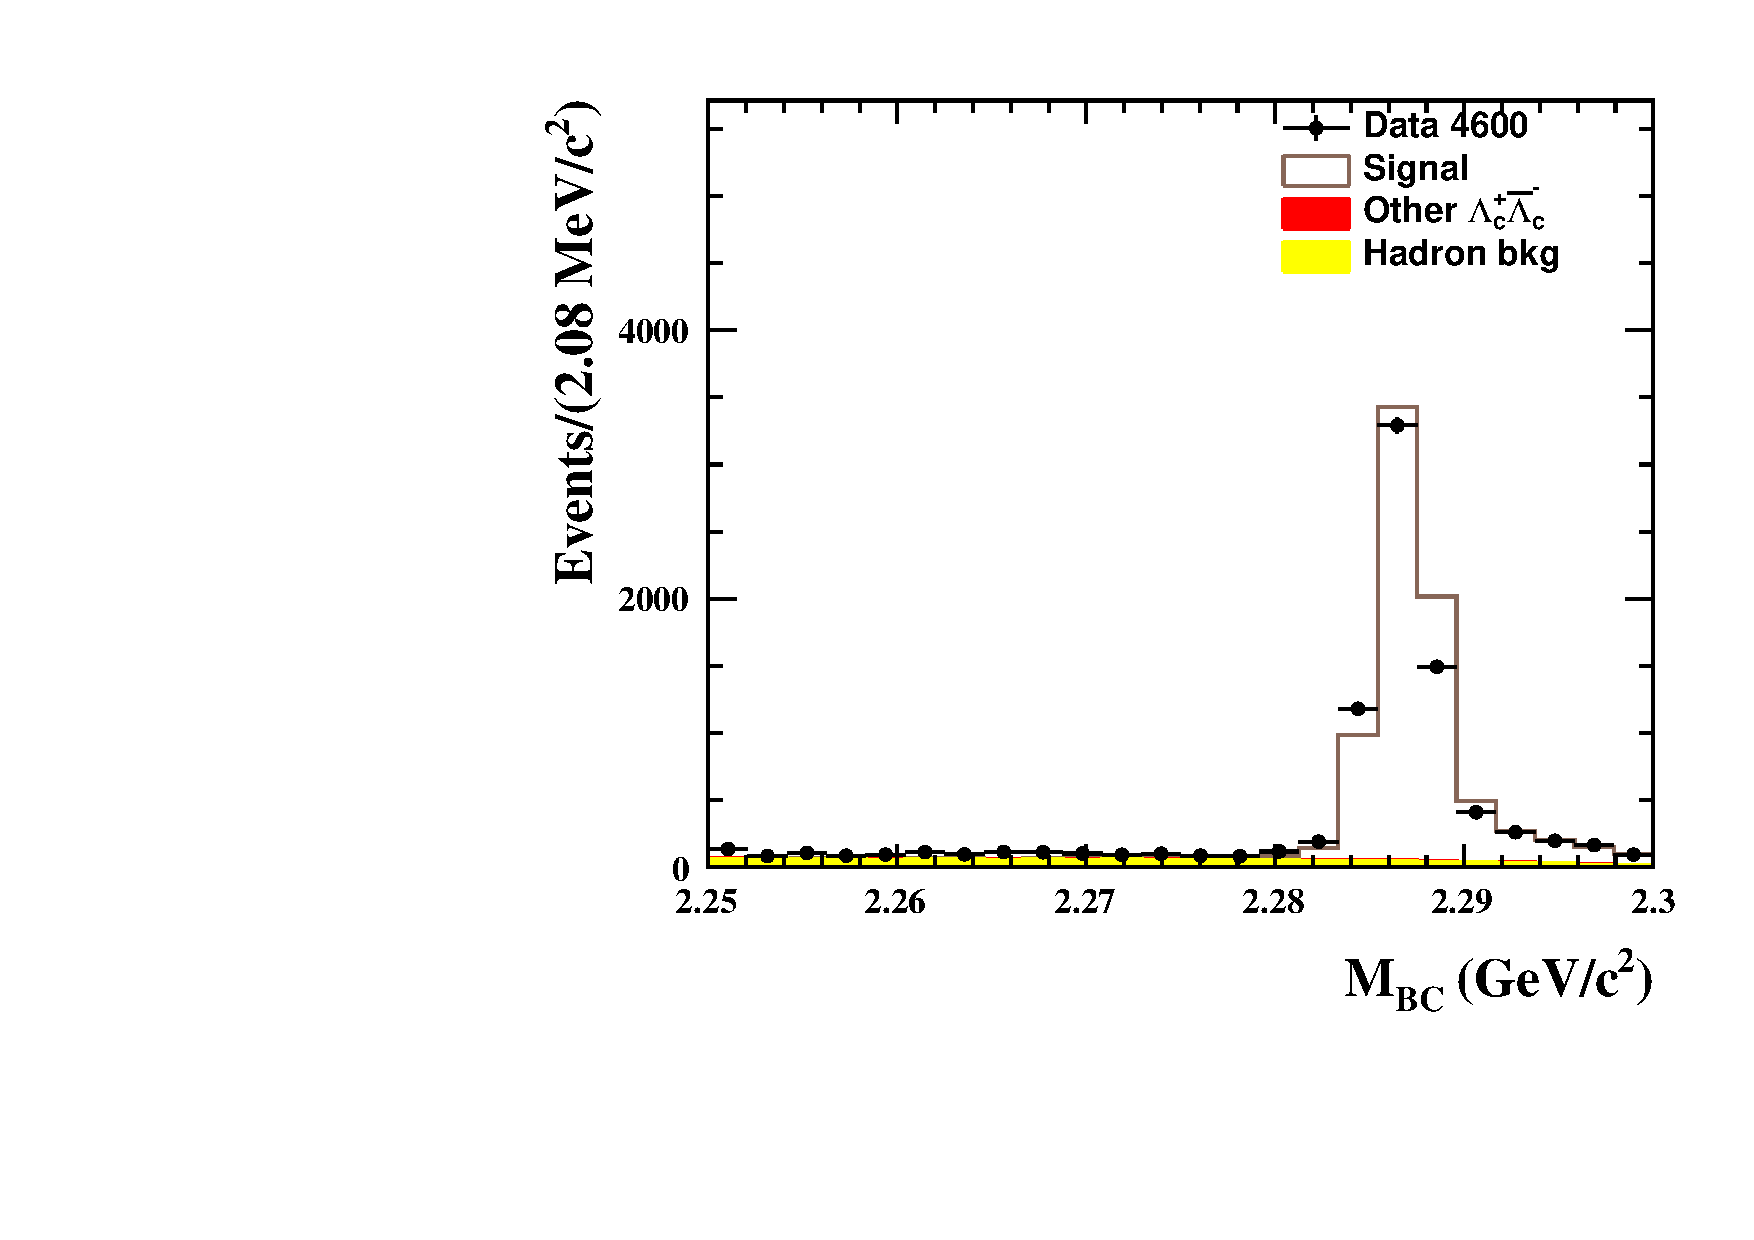
\includegraphics[width=0.24\textwidth]{figure/full_mbc/output_4600_mBC.pdf}
    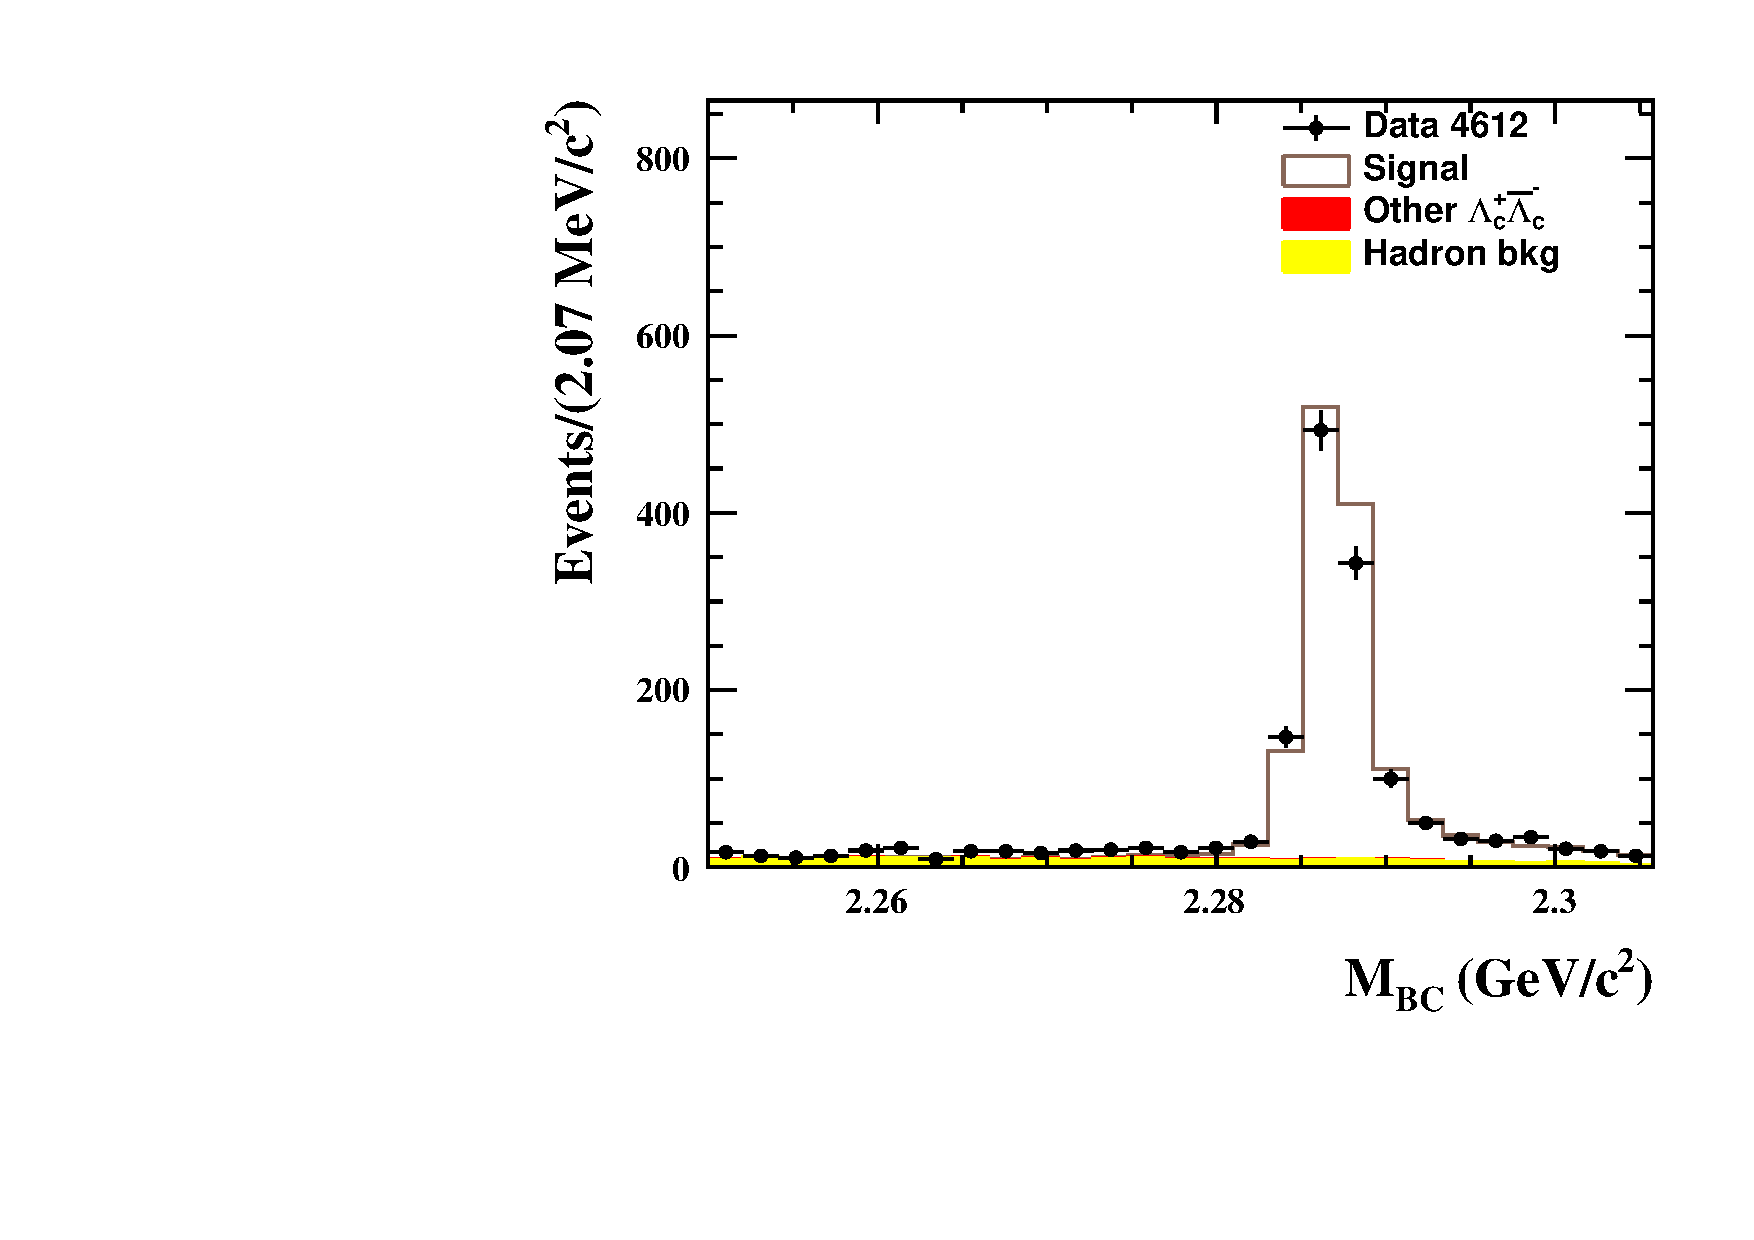
\includegraphics[width=0.24\textwidth]{figure/full_mbc/output_4612_mBC.pdf}
    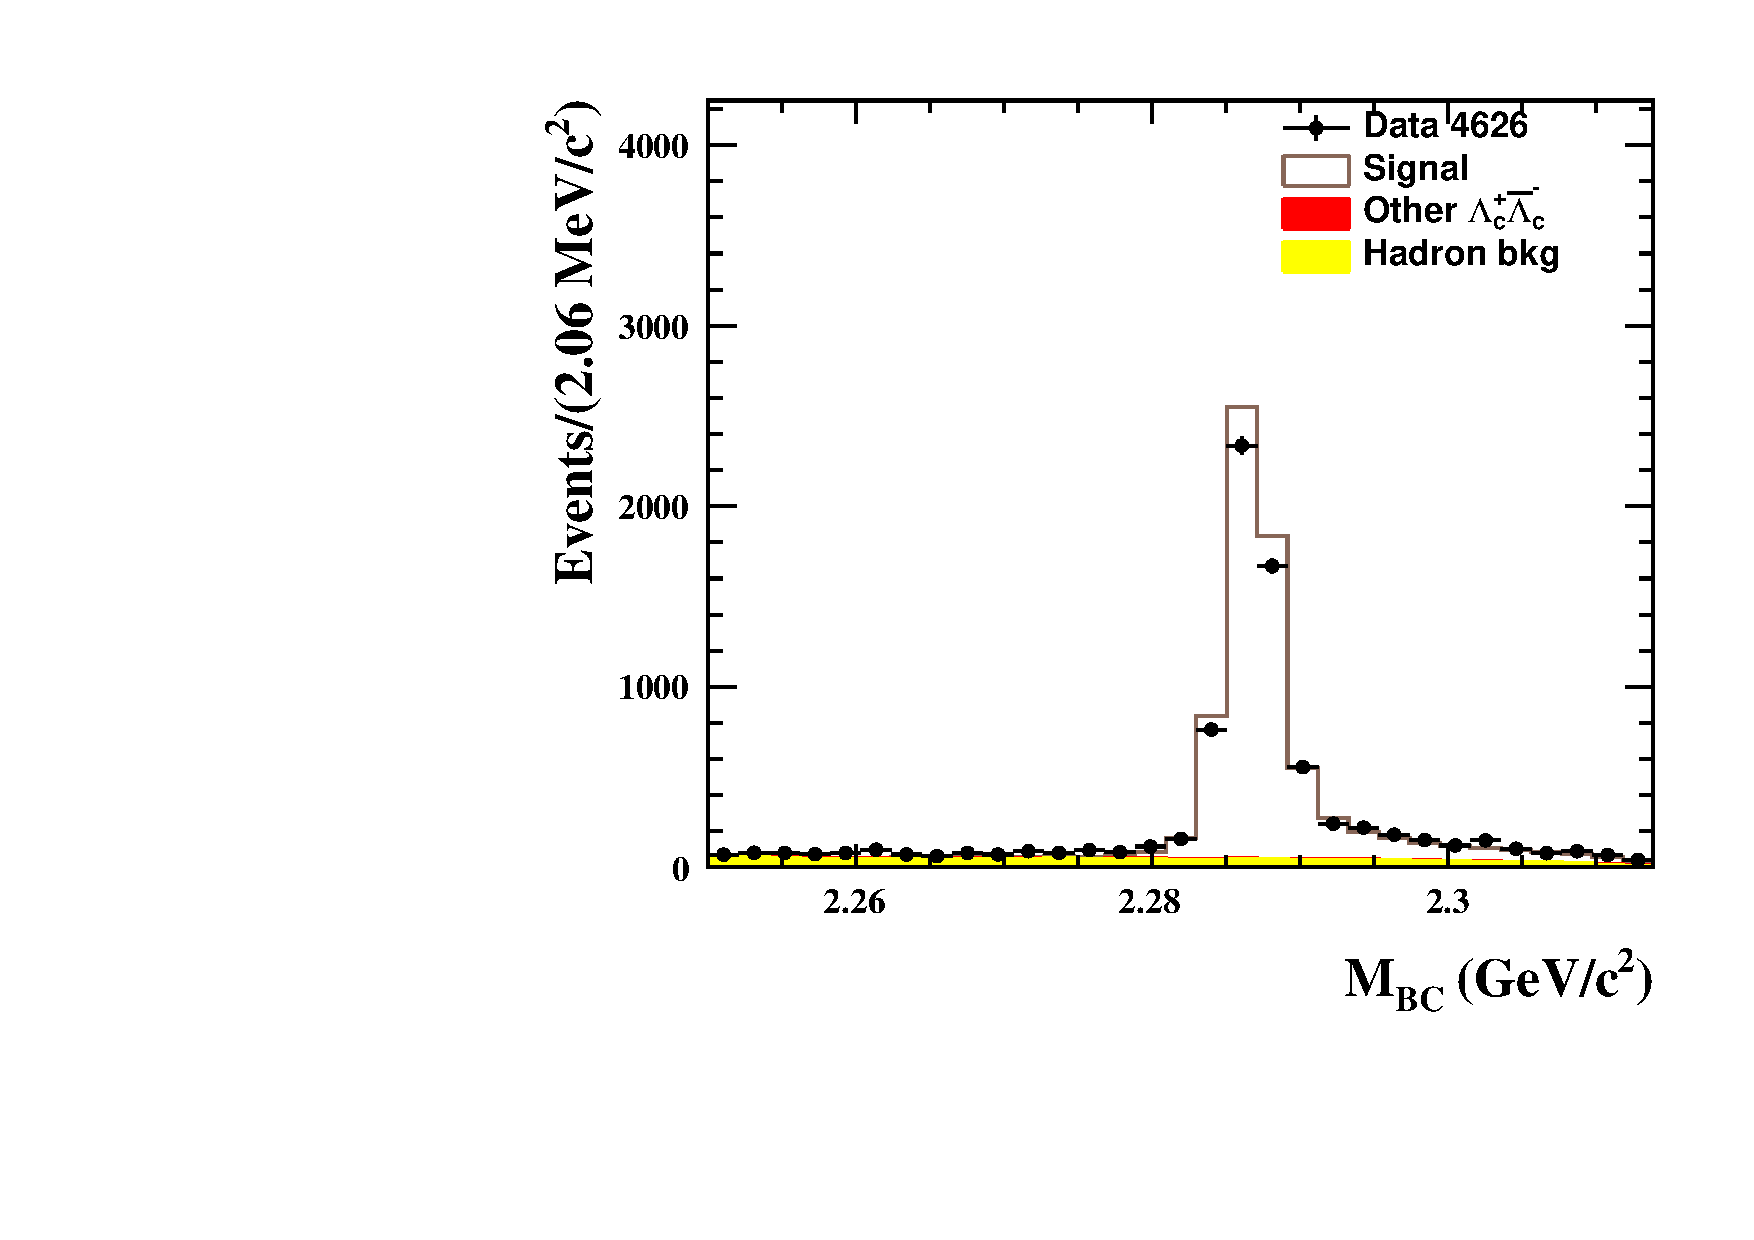
\includegraphics[width=0.24\textwidth]{figure/full_mbc/output_4626_mBC.pdf}
    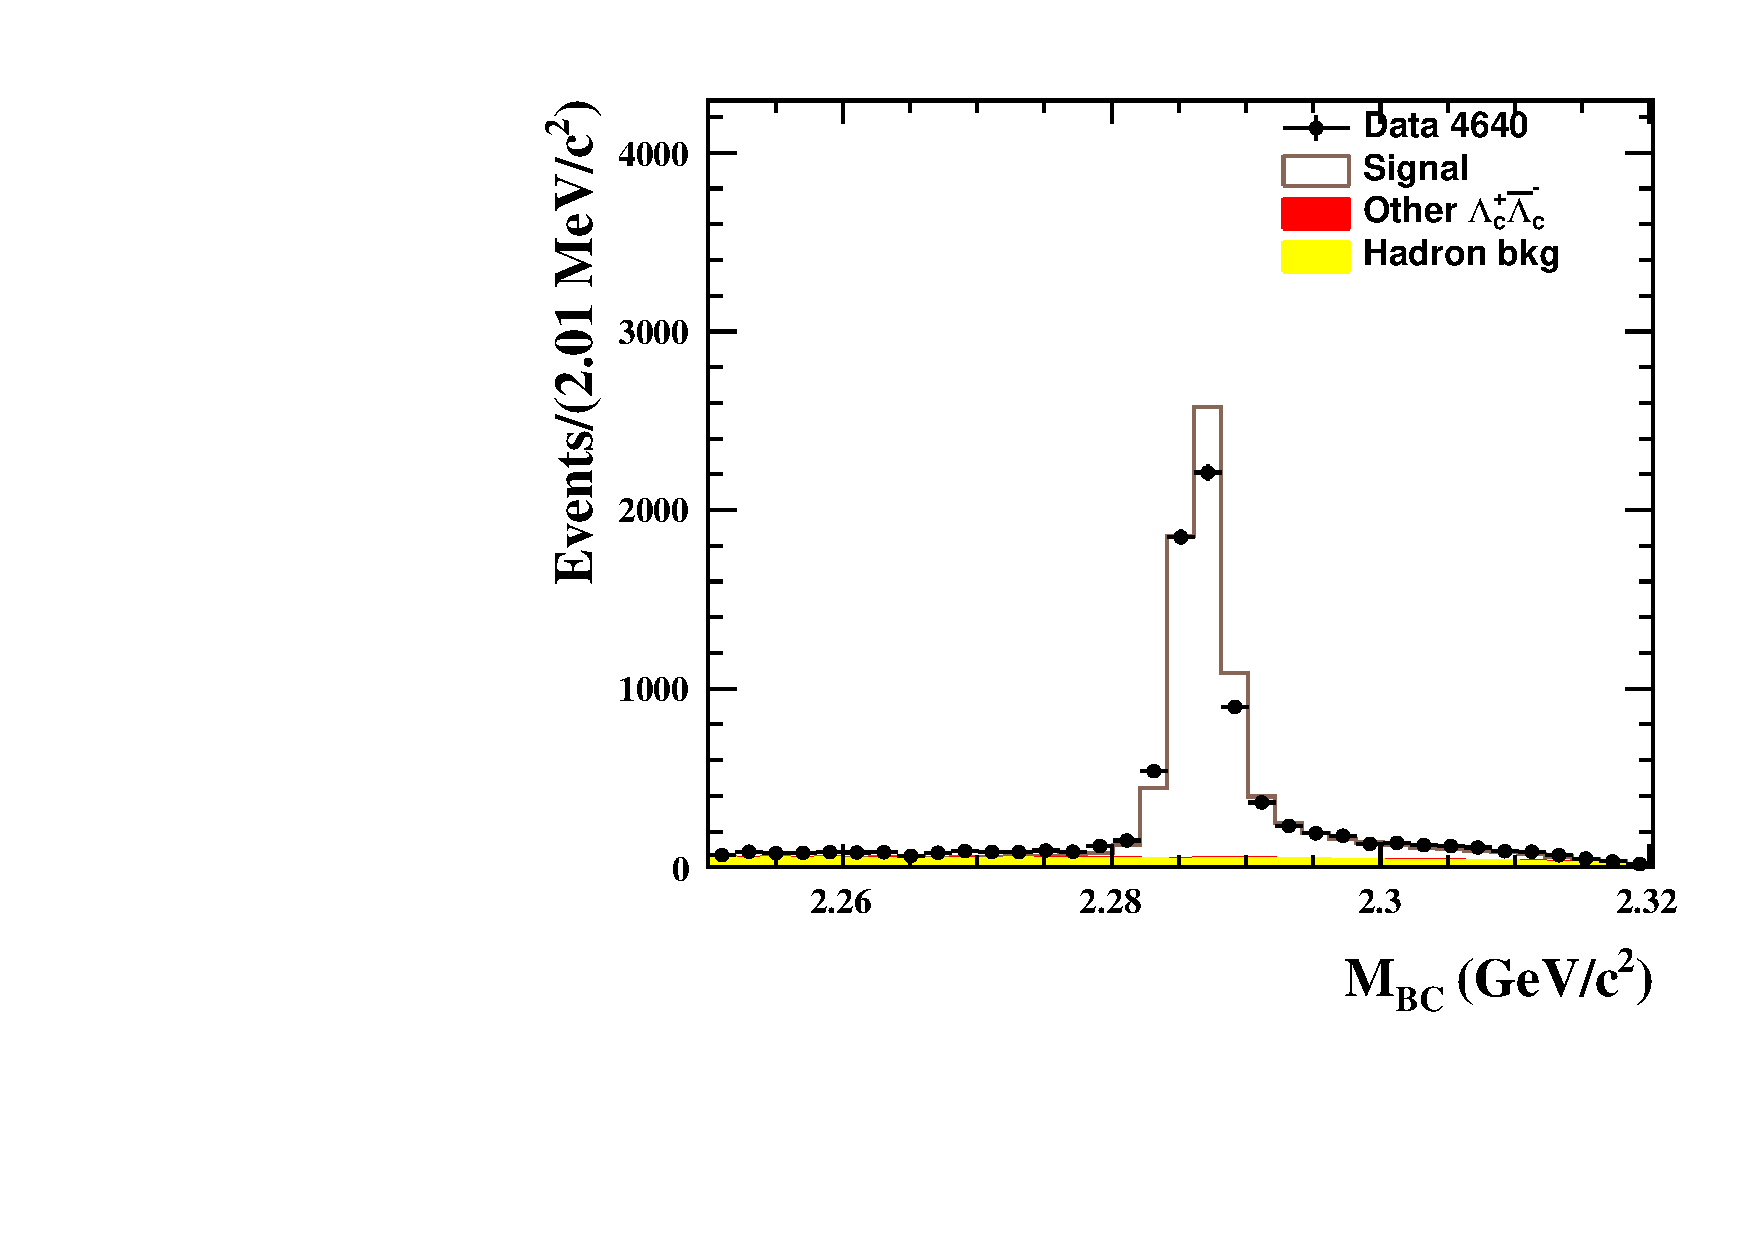
\includegraphics[width=0.24\textwidth]{figure/full_mbc/output_4640_mBC.pdf}
    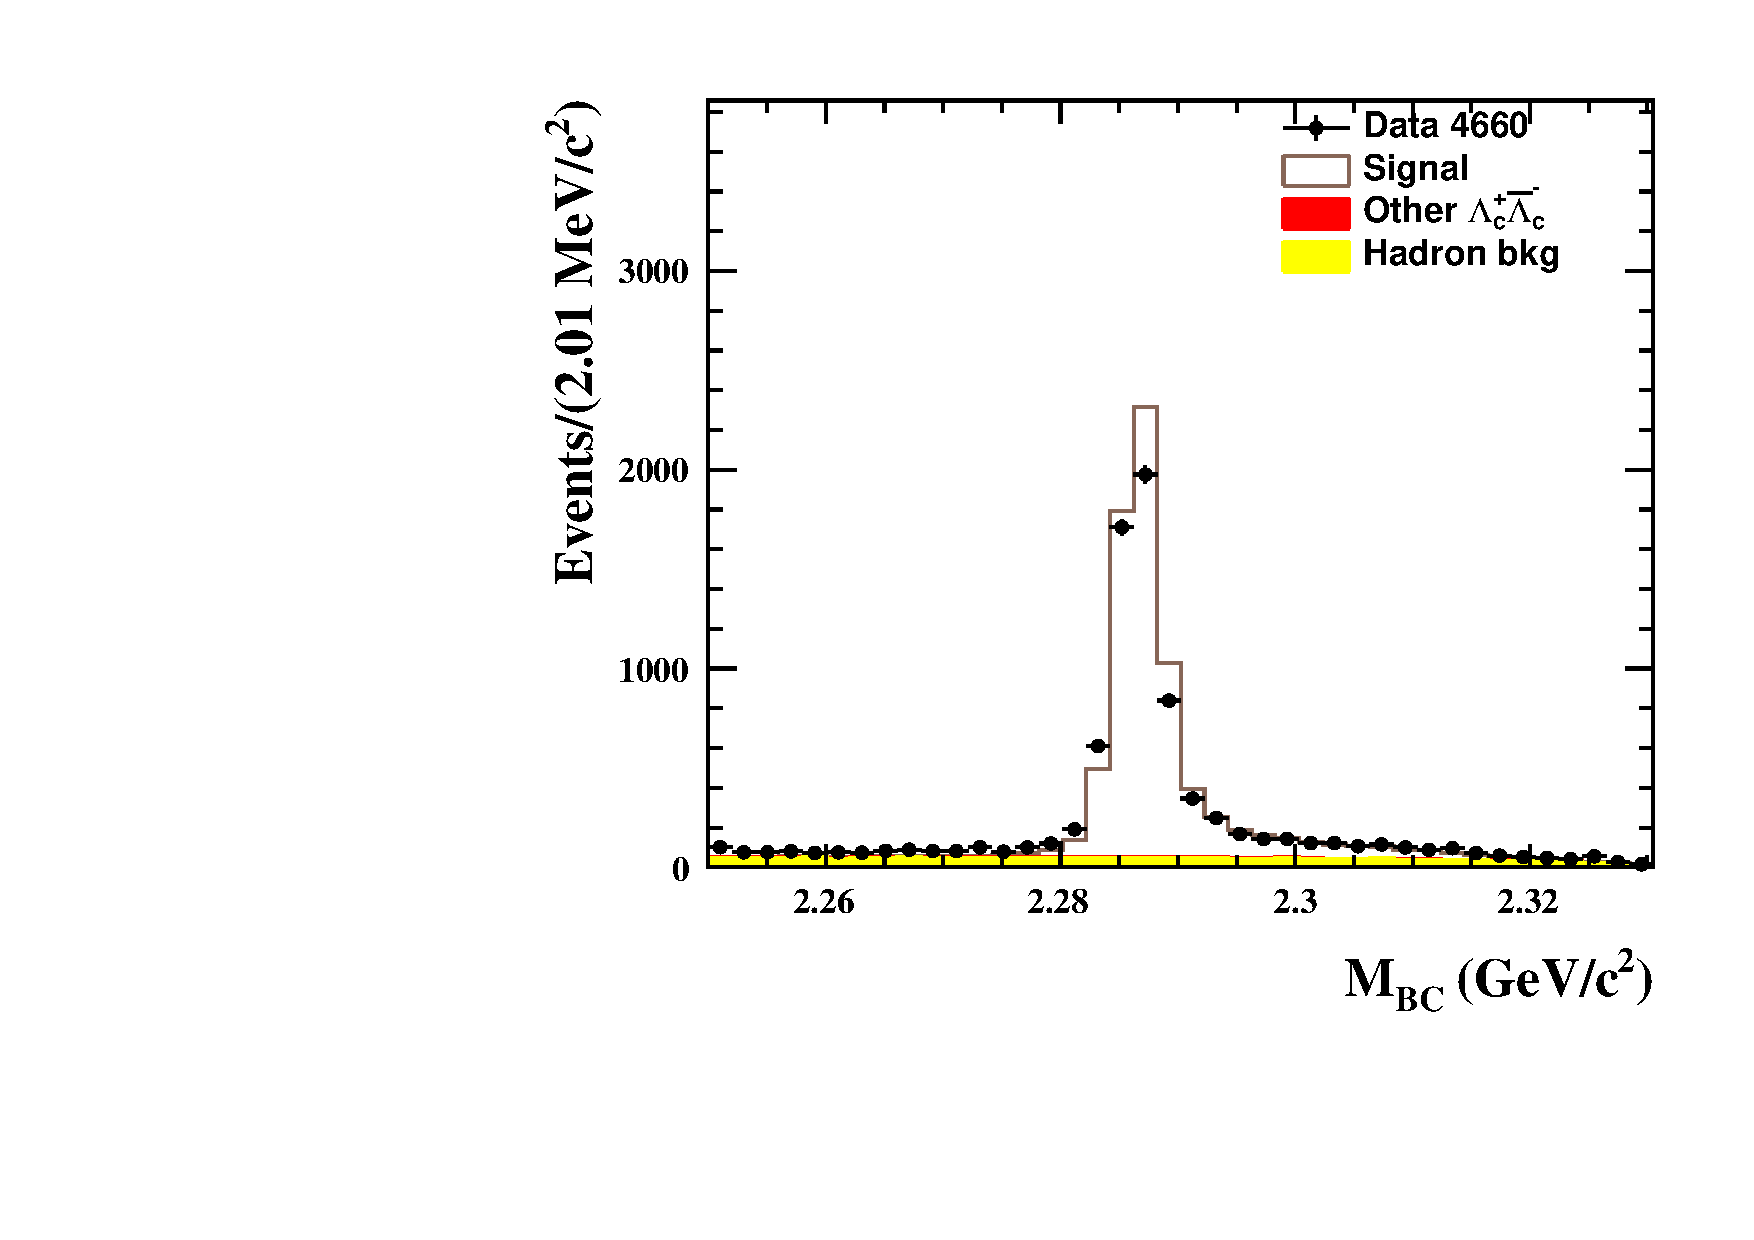
\includegraphics[width=0.24\textwidth]{figure/full_mbc/output_4660_mBC.pdf}
    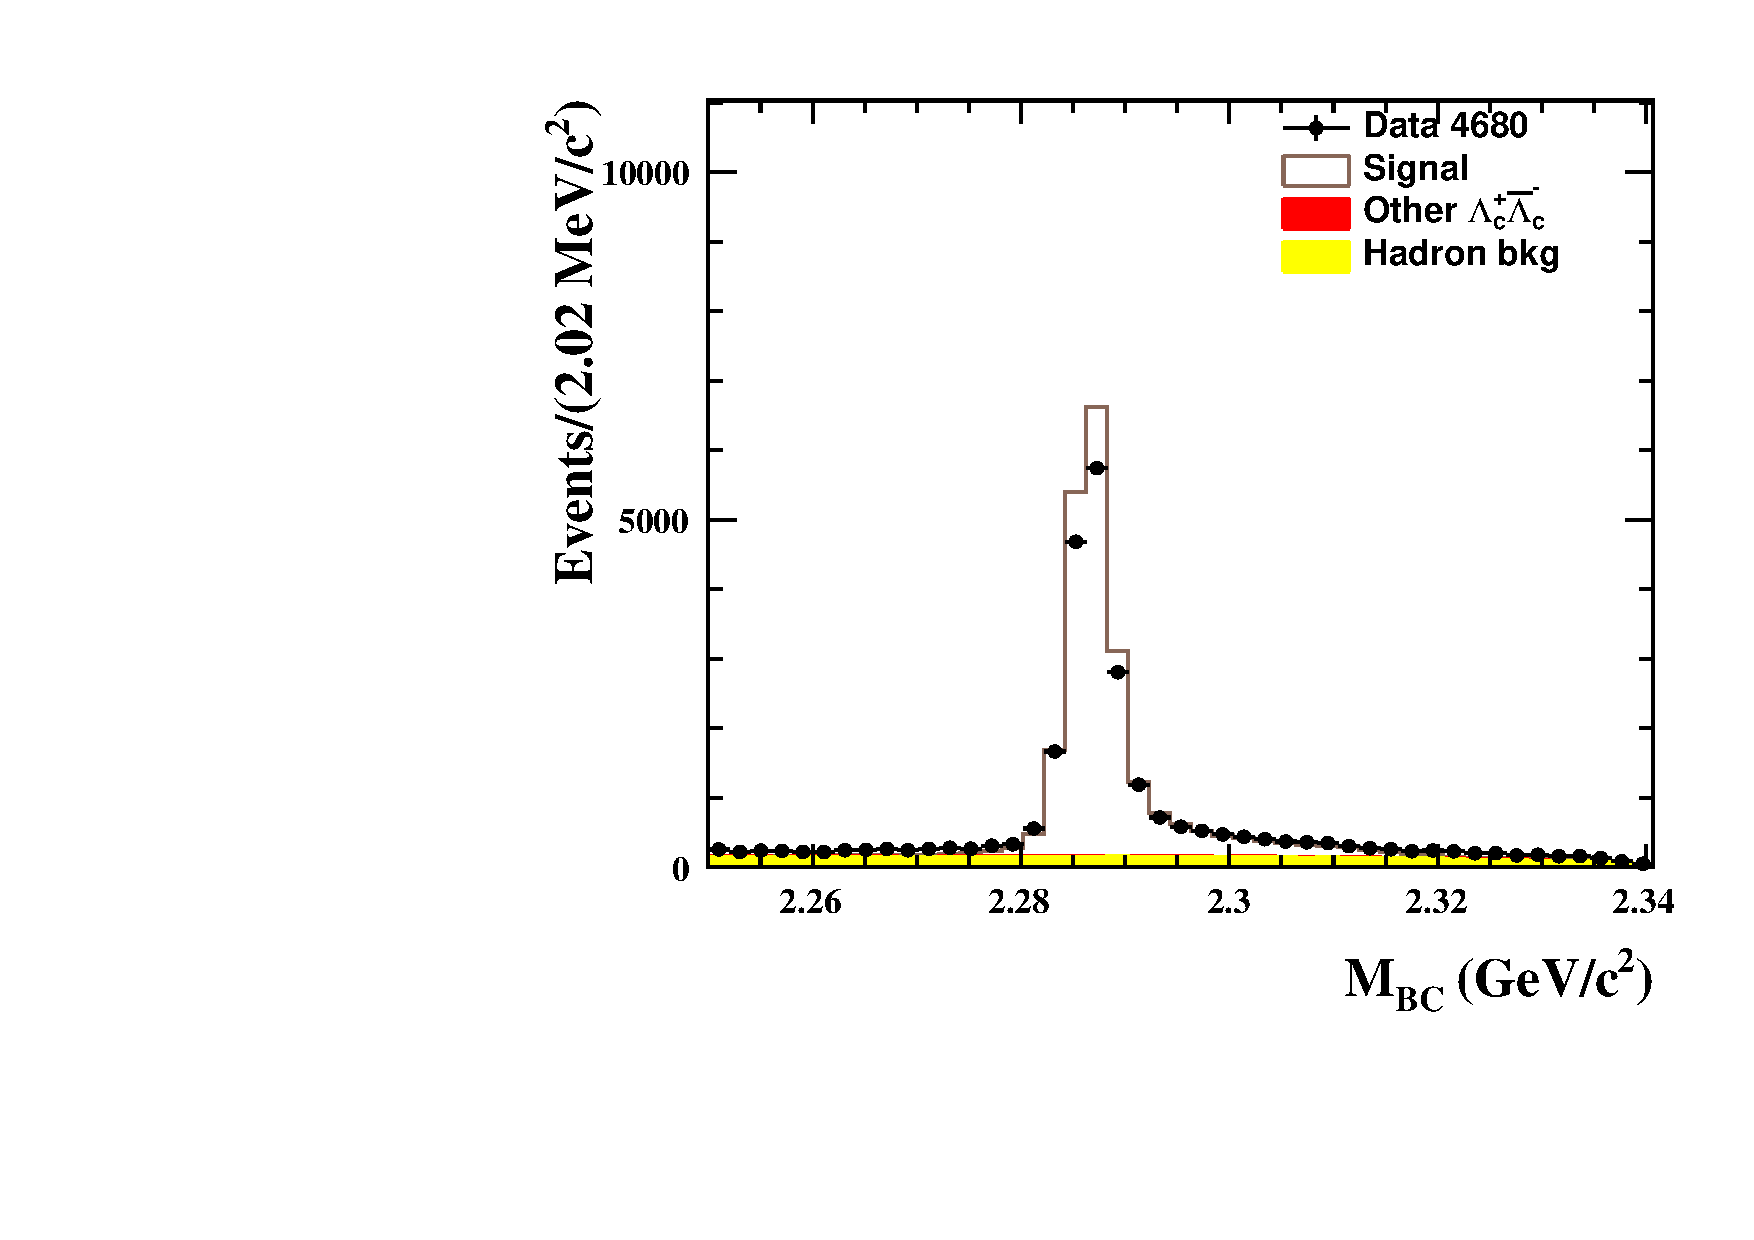
\includegraphics[width=0.24\textwidth]{figure/full_mbc/output_4680_mBC.pdf}
    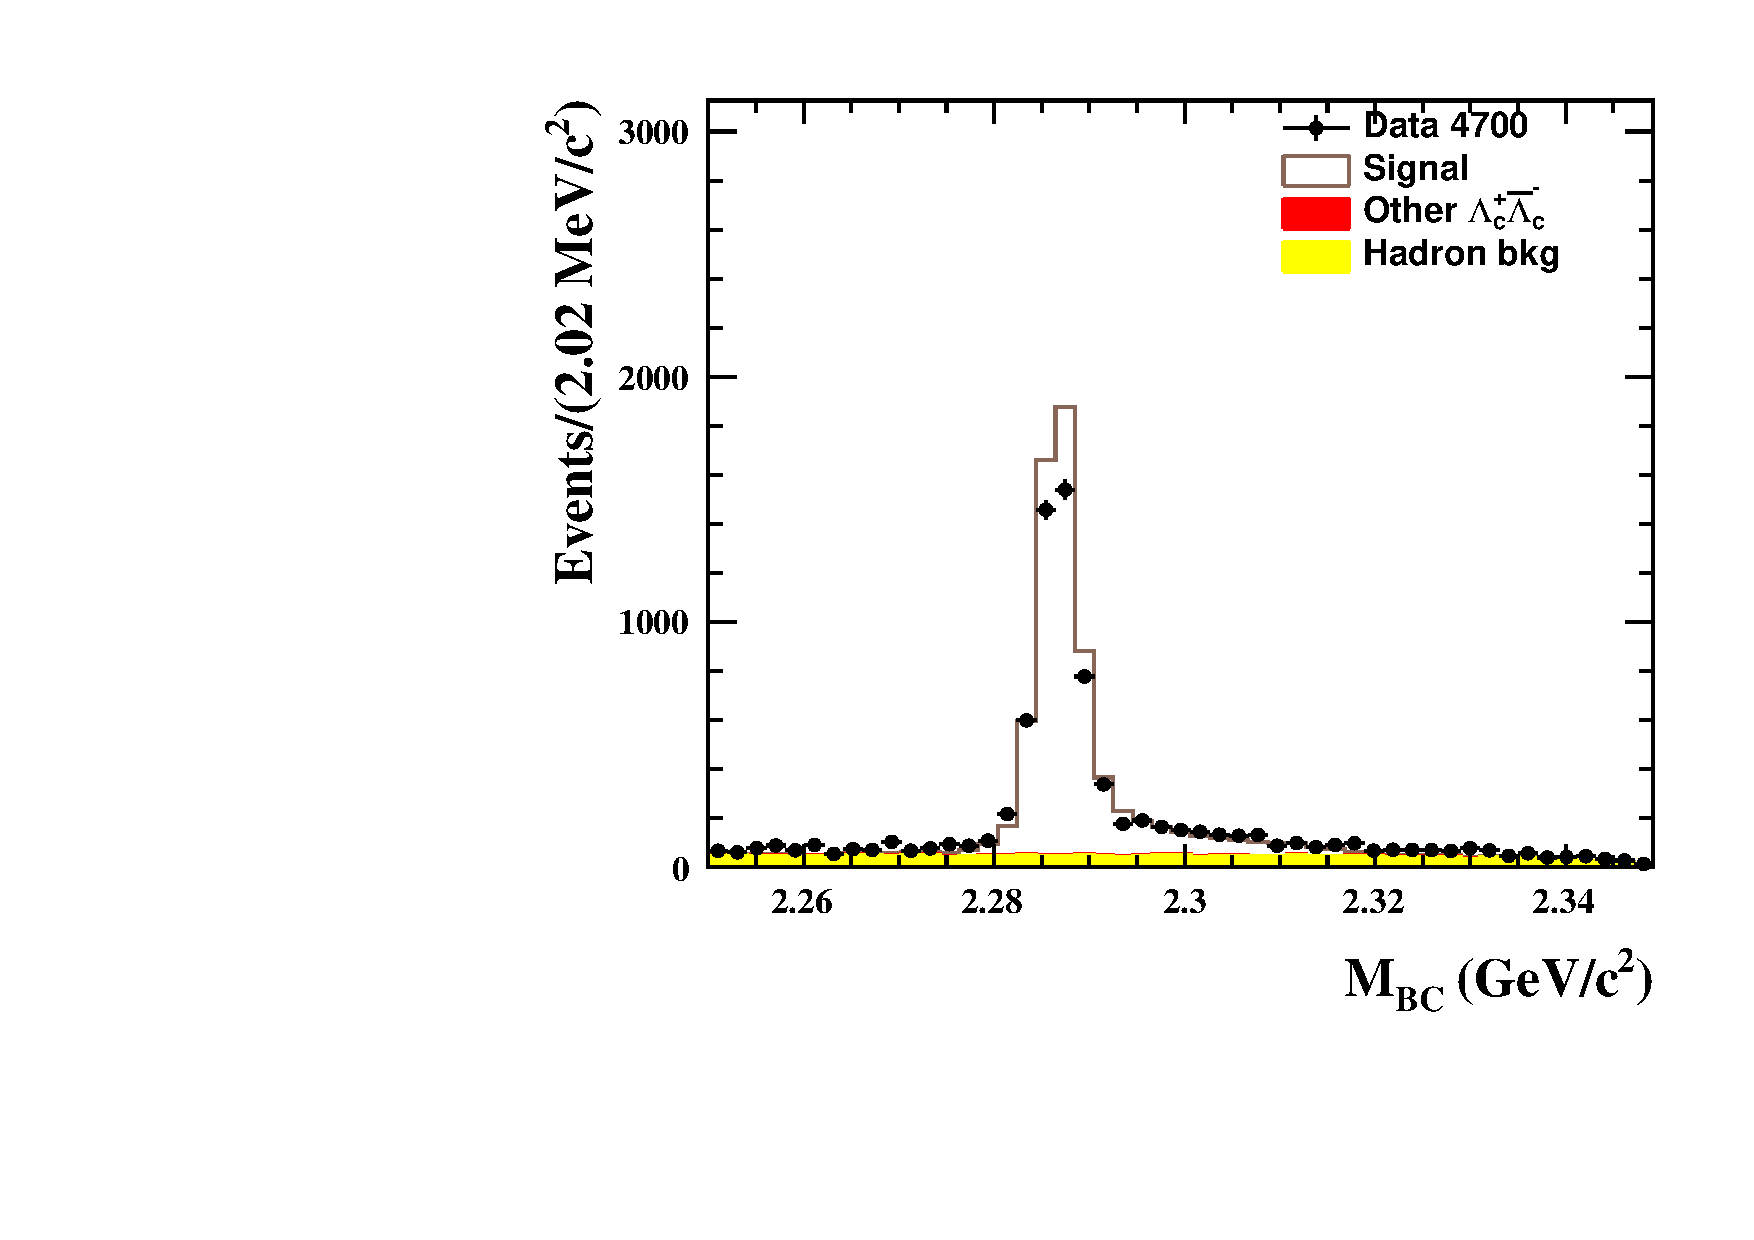
\includegraphics[width=0.24\textwidth]{figure/full_mbc/output_4700_mBC.pdf}
    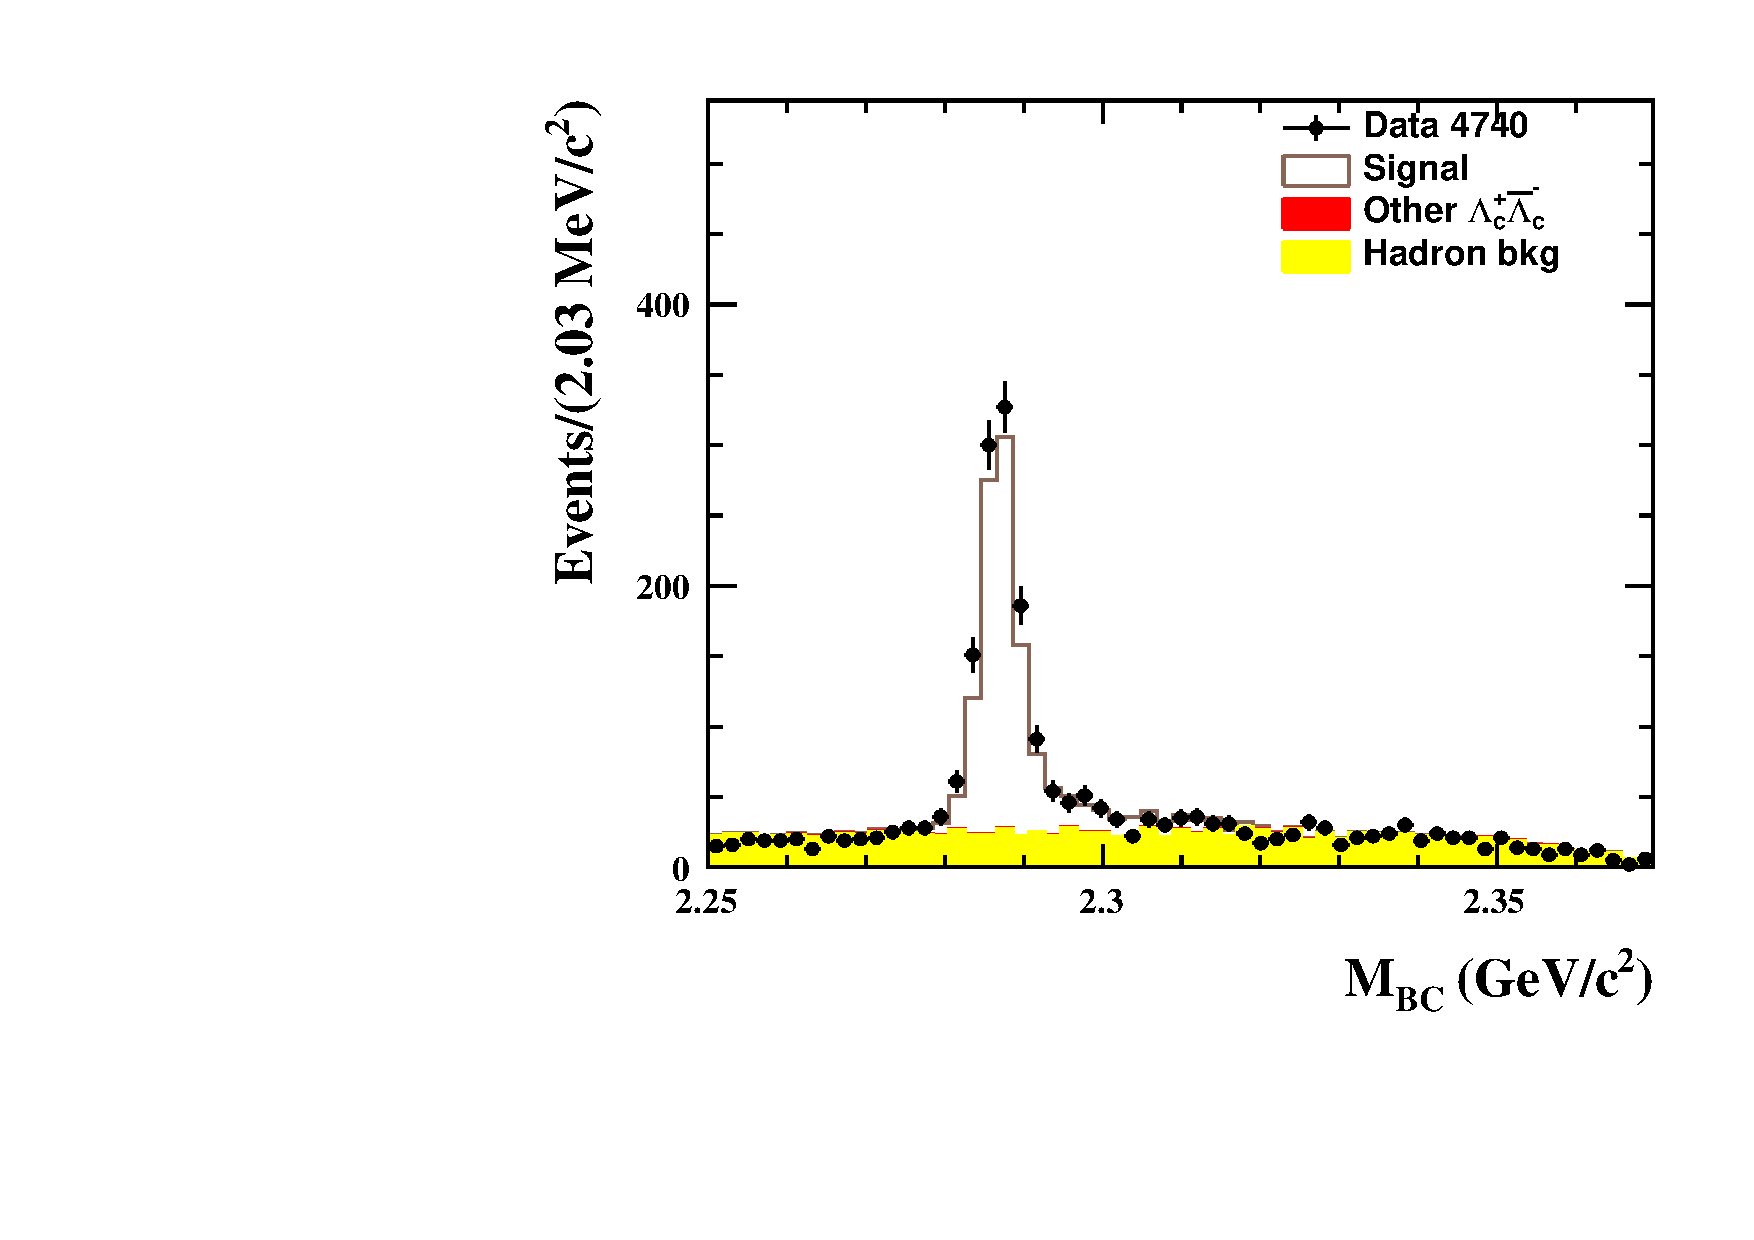
\includegraphics[width=0.24\textwidth]{figure/full_mbc/output_4740_mBC.pdf}
    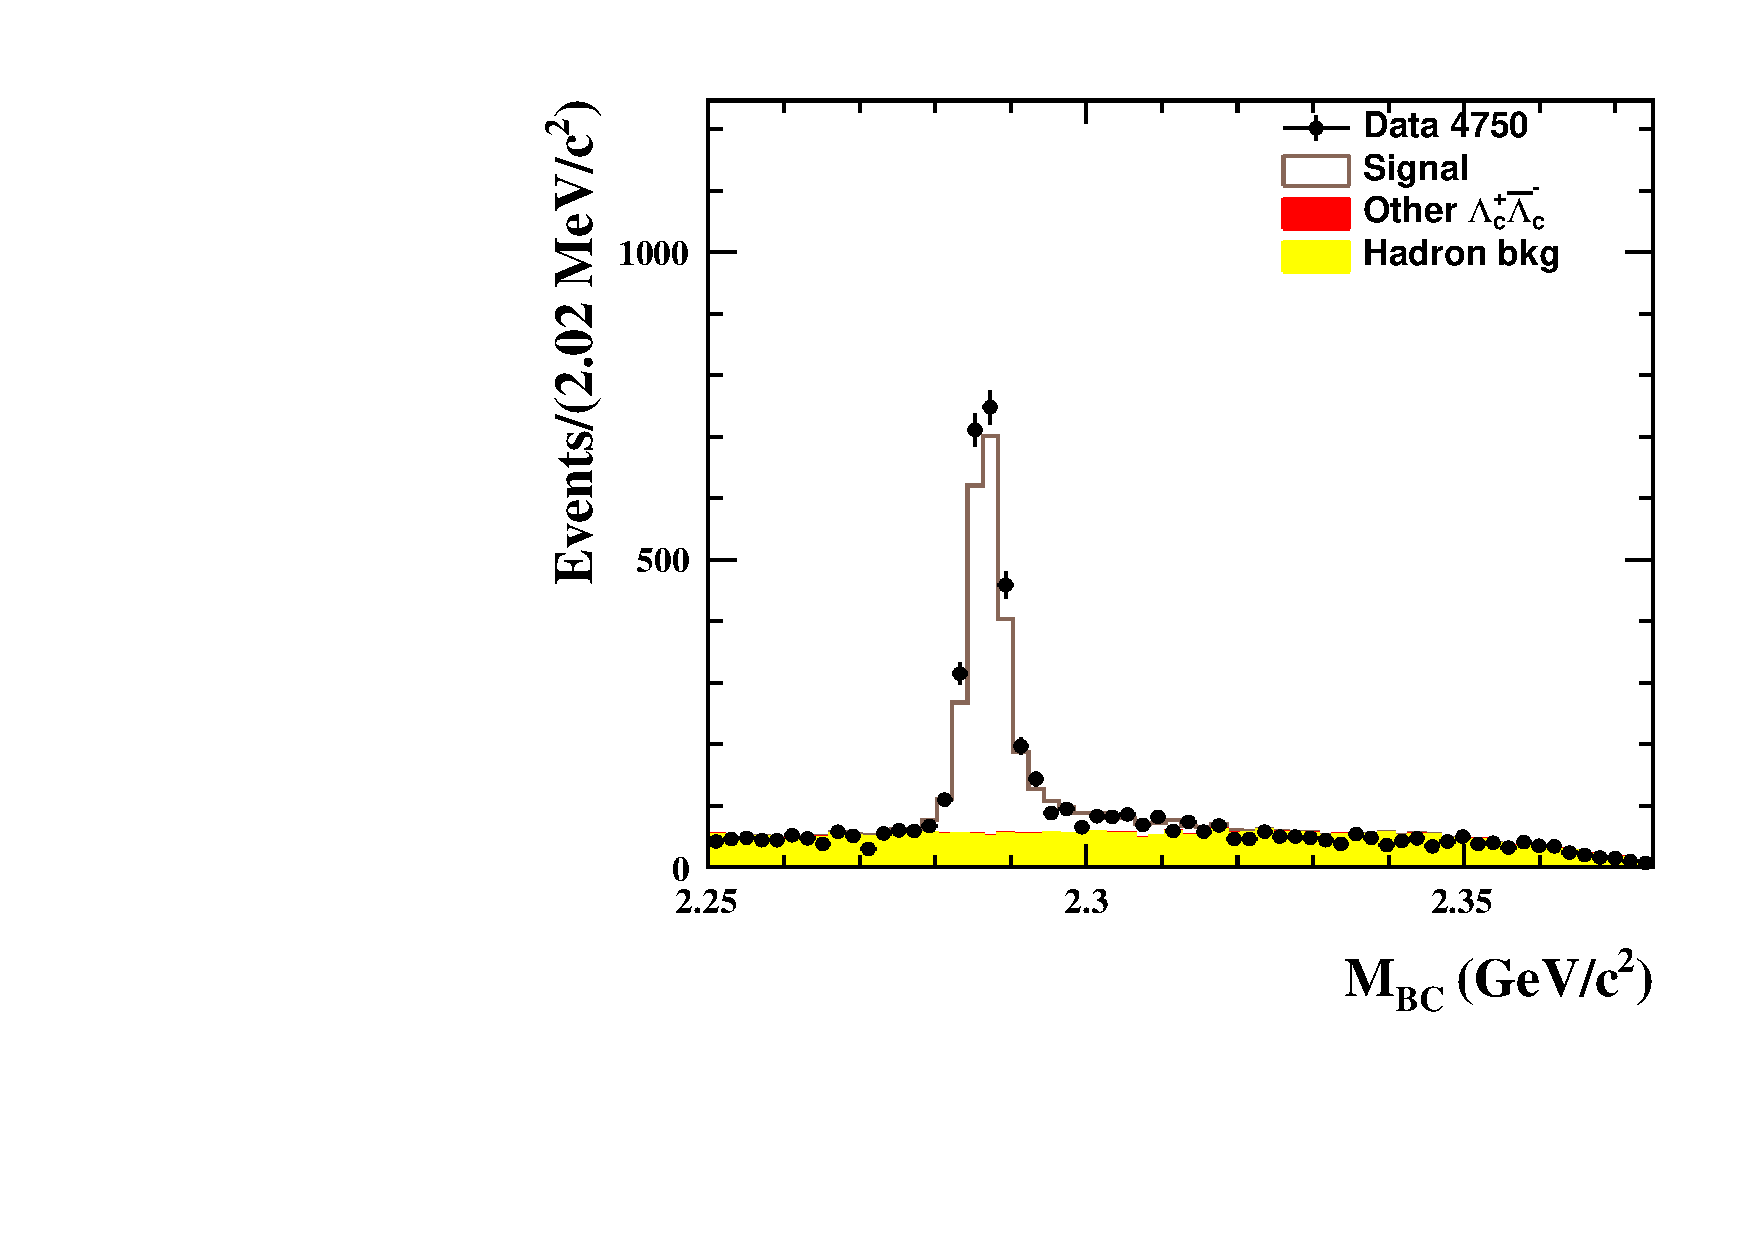
\includegraphics[width=0.24\textwidth]{figure/full_mbc/output_4750_mBC.pdf}
    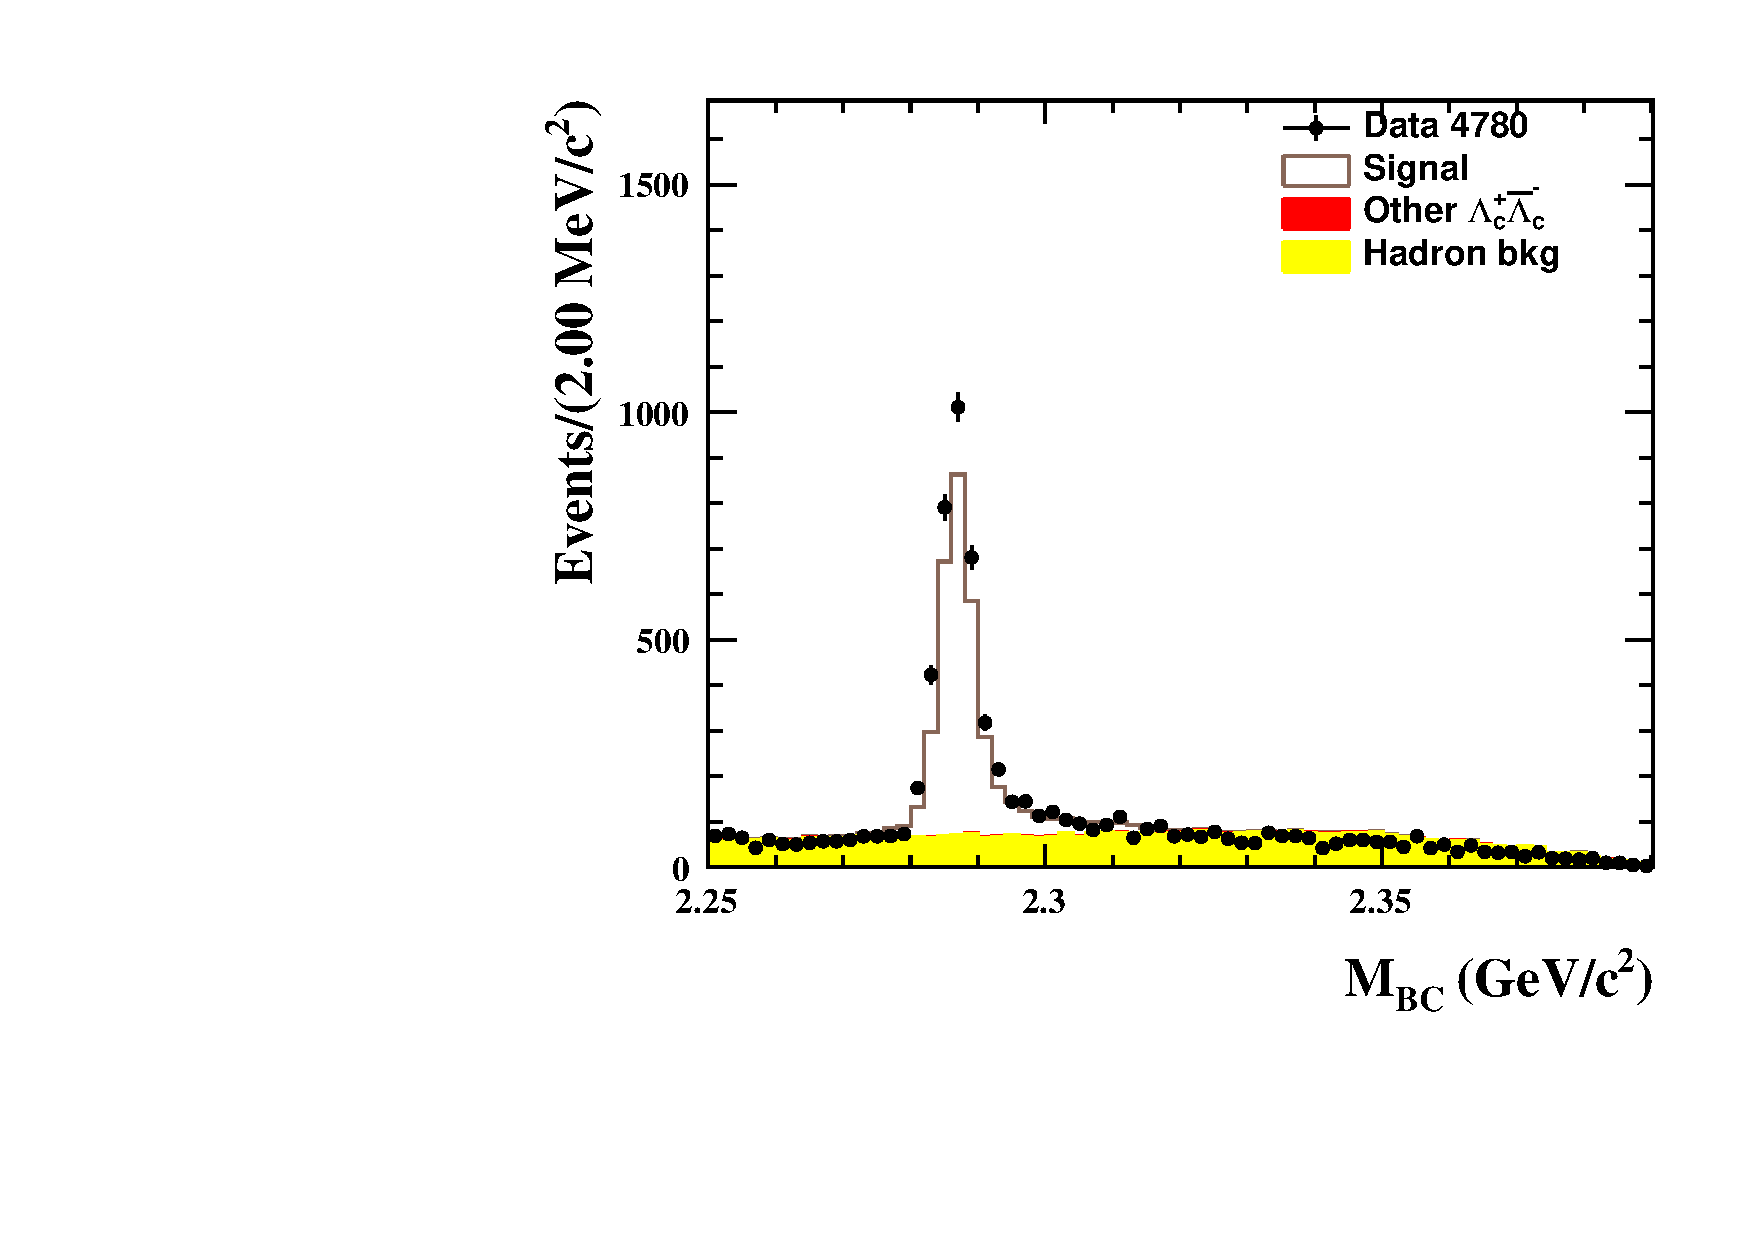
\includegraphics[width=0.24\textwidth]{figure/full_mbc/output_4780_mBC.pdf}
    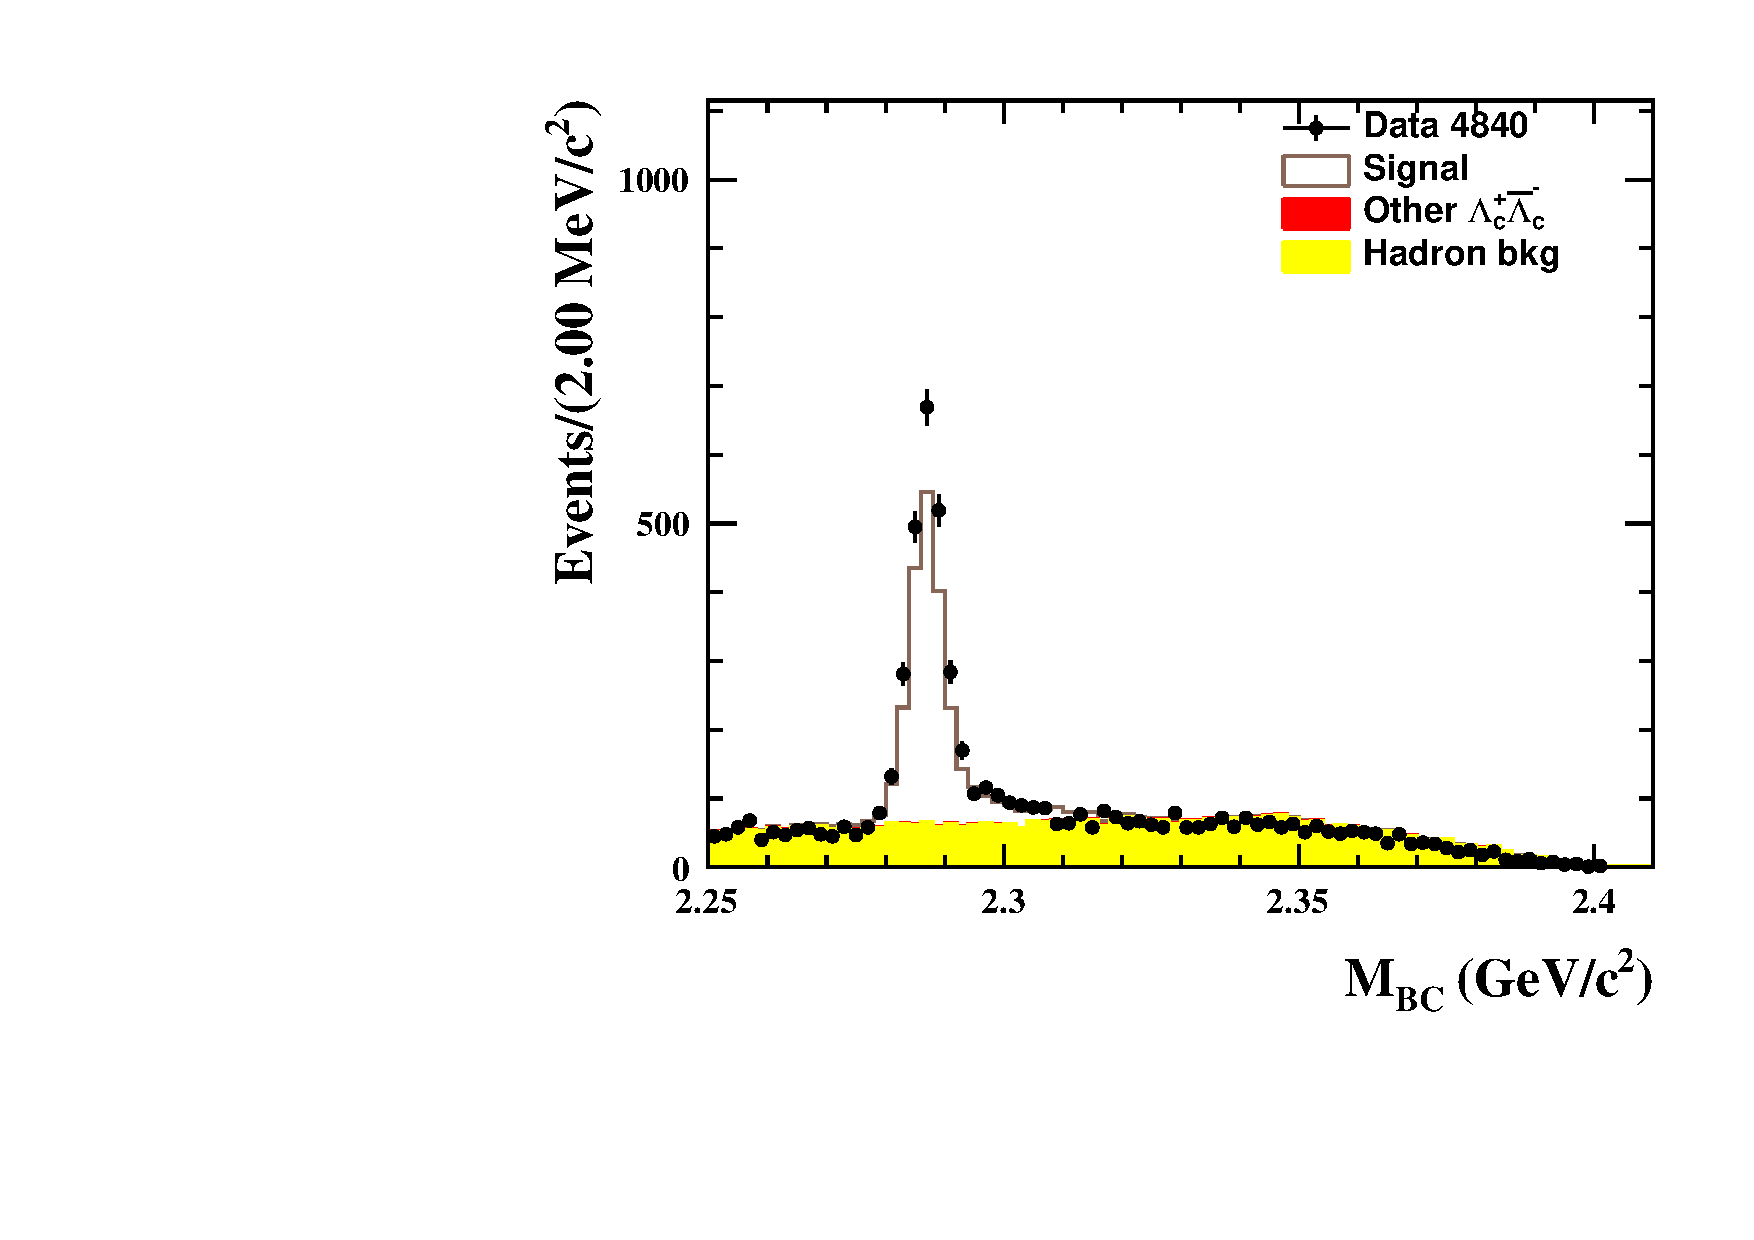
\includegraphics[width=0.24\textwidth]{figure/full_mbc/output_4840_mBC.pdf}
    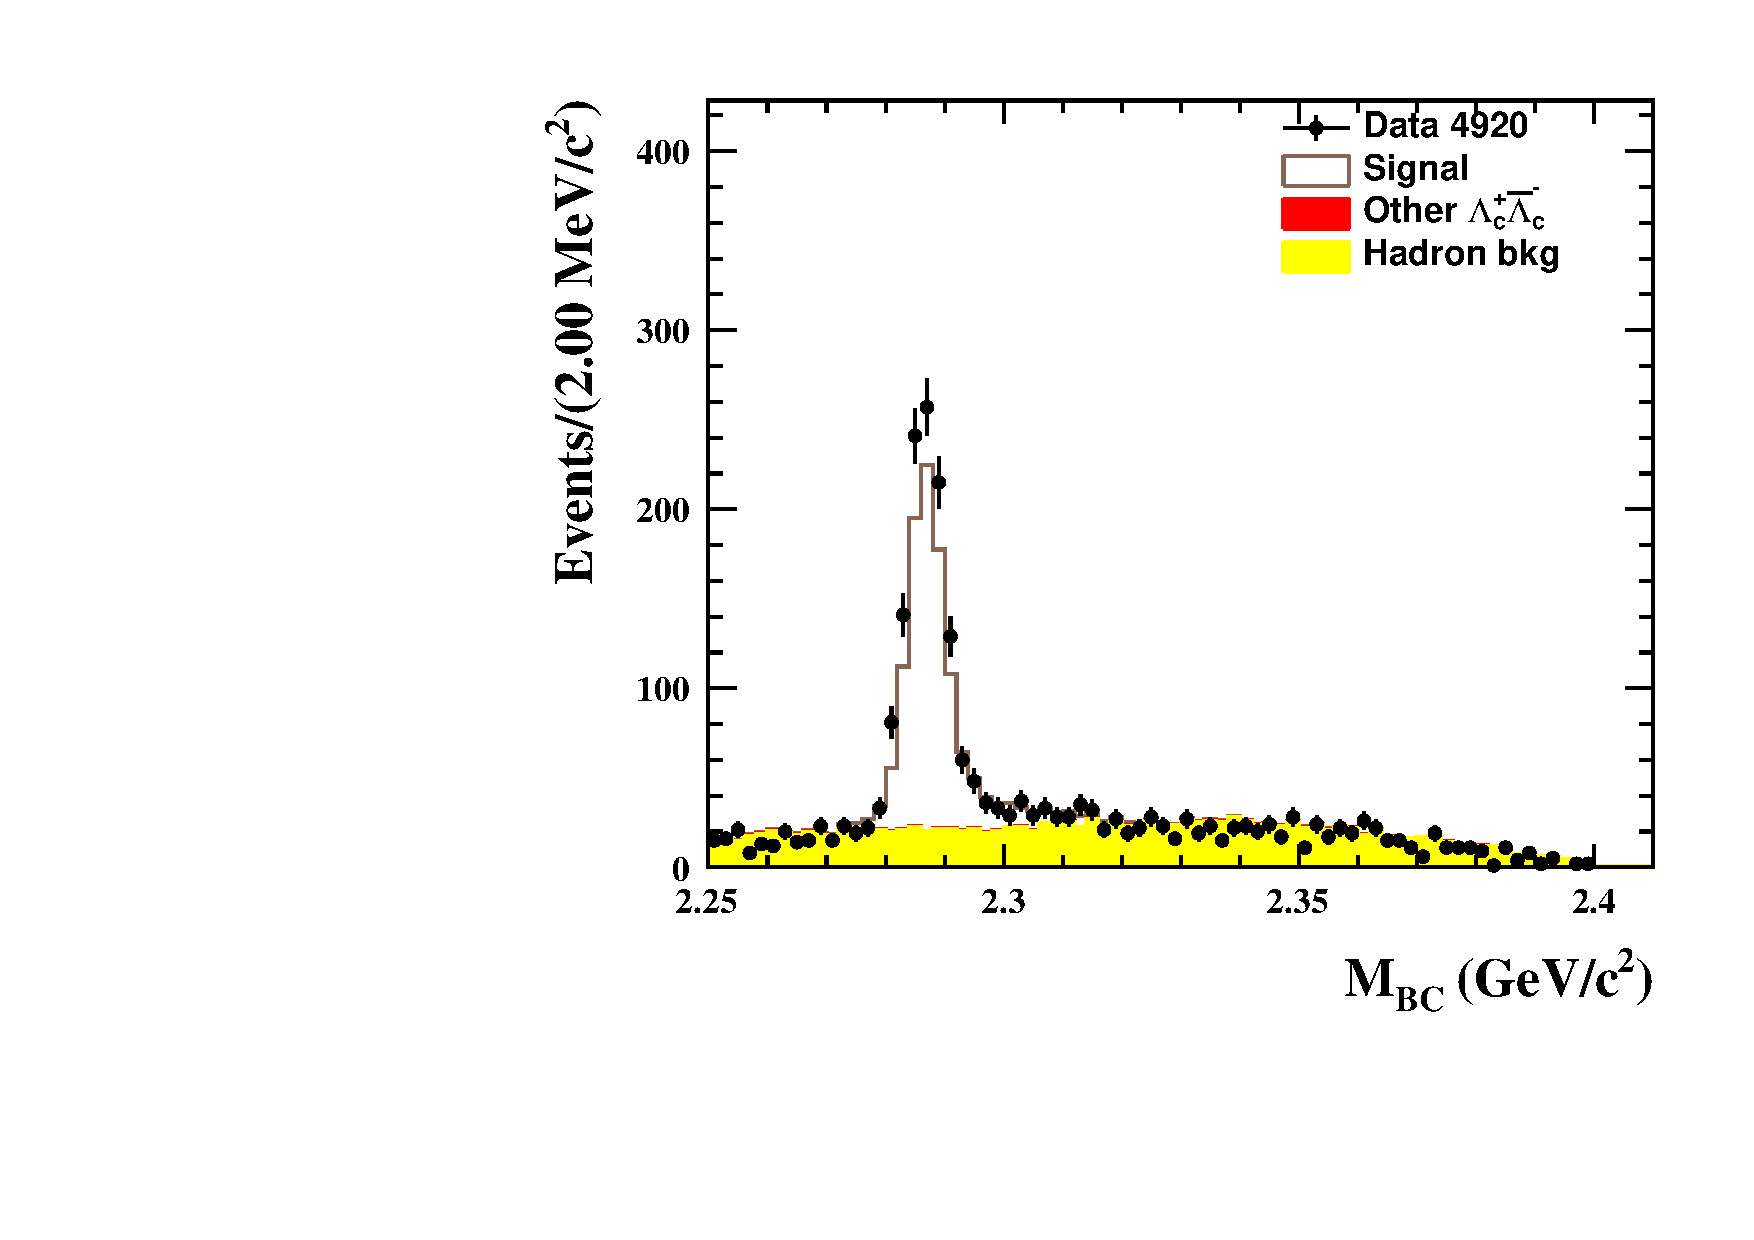
\includegraphics[width=0.24\textwidth]{figure/full_mbc/output_4914_mBC.pdf}
    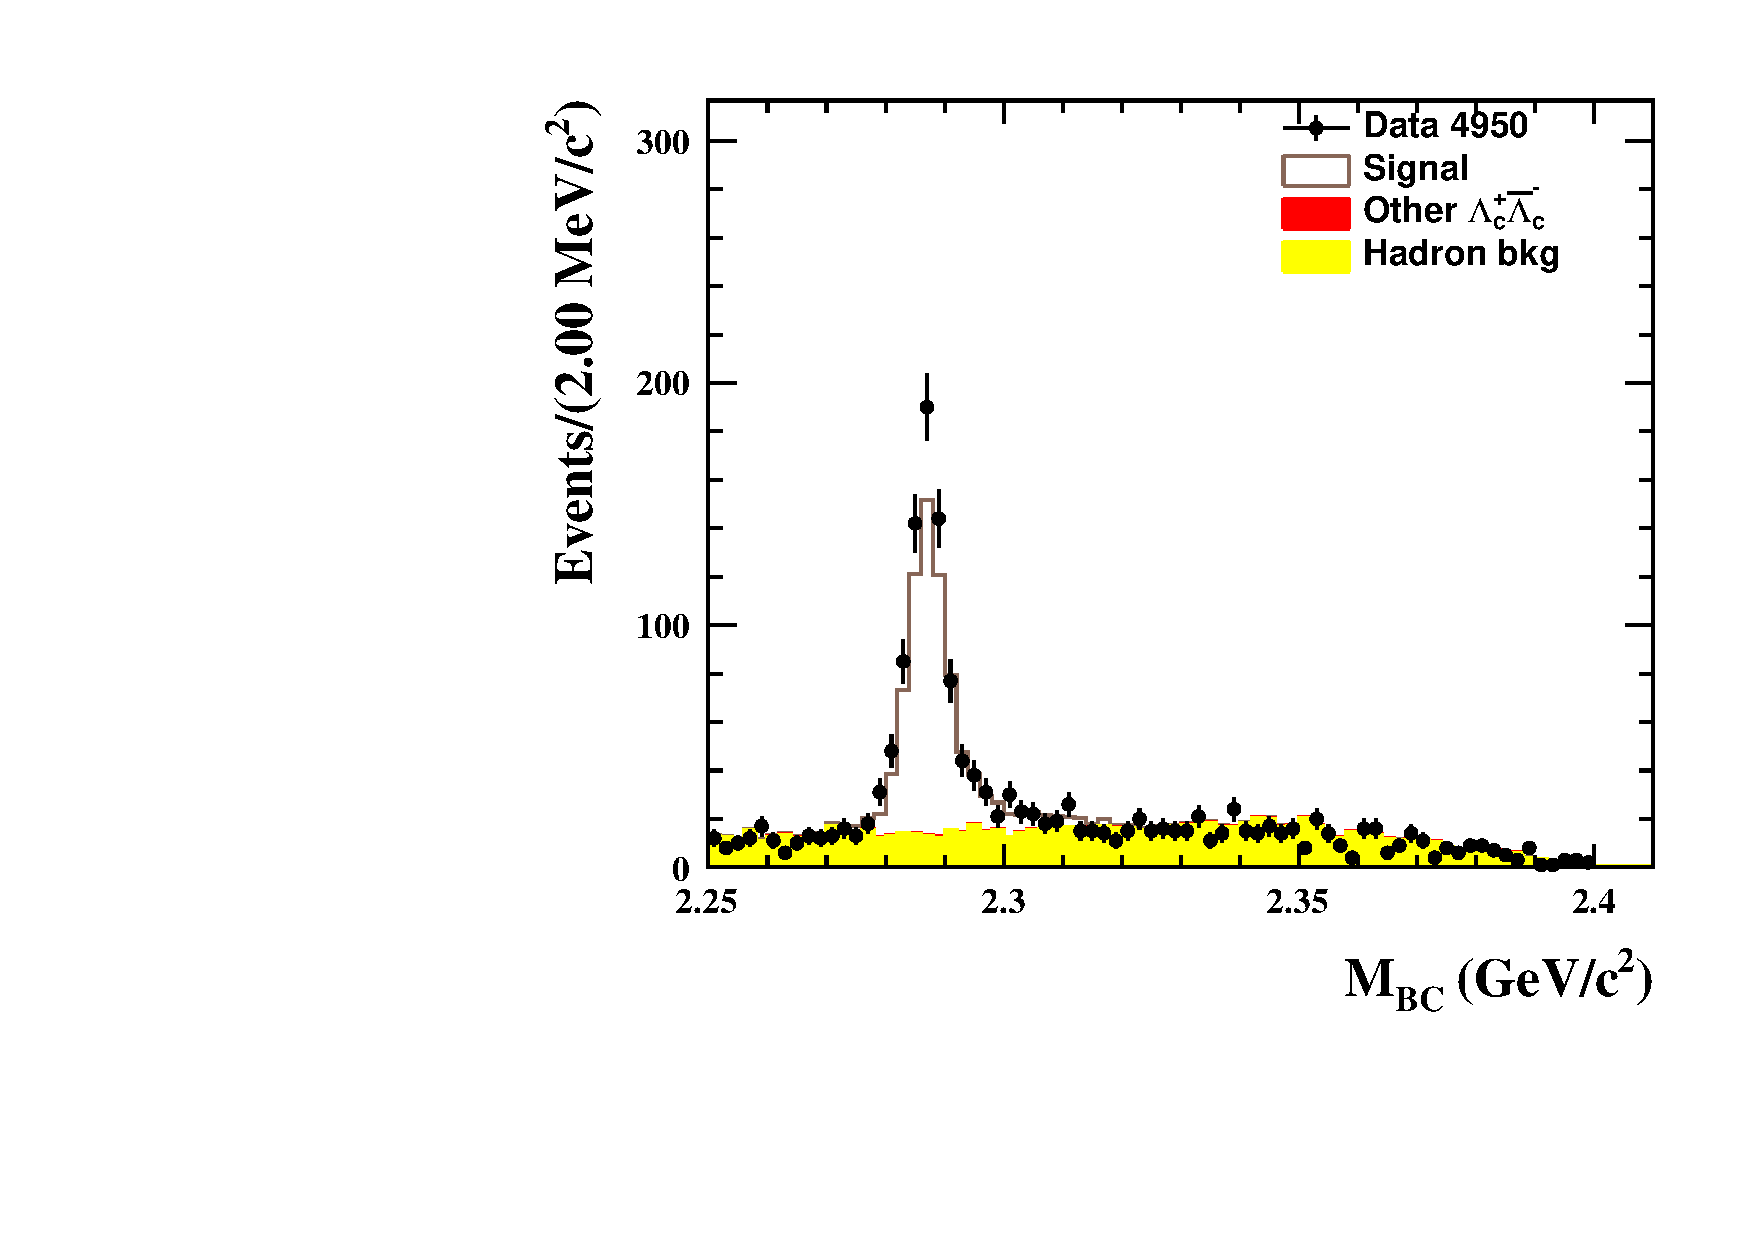
\includegraphics[width=0.24\textwidth]{figure/full_mbc/output_4946_mBC.pdf}
    \caption{Comparison of data and cocktail MC samples for each energy point. The cocktail MC samples are scaled to the integrated luminosity of data.}
\label{fig:full_mbc}
\end{figure}

\subsection{ST signal yields}
\label{sec:st_yields}

Extended unbinned maximum likelihood fits are conducted to extract the single-tag (ST) signal yields and purity from the $\mbc$ distributions across all energy points. In the fit, %the signal shape is derived from the kernel-estimated non-parametric shape~\cite{Cranmer:2000du} of the invisible PHSP signal MC samples. 
the signal shape is extracted from the invisible PHSP signal MC samples using RooKeysPdf tool. To account for the discrepancies between data and MC simulations, a Gaussian function with adjustable parameters is convolved with the signal shape. For energy points below $\sqrt{s} = 4.740\gev/c^2$, the background shape is described by the ARGUS~\cite{Djouadi:1989hh} function, defined as follows:
\begin{equation}
P_{\rm bkg}(\mbc,E_0,c,p) = \mbc \left(1 - \left(\frac{\mbc}{E_0}\right)^2 \right)^p \times e^{c \left(1-\frac{\mbc}{E_0}\right)^2},
\end{equation}
where $E_0$ represents the endpoint of $\mbc$ and is fixed at the beam energy. The parameters $p$ and $c$ correspond to the power parameter and the scale factor, respectively. The default value for $p$ is set to 0.5 and is held fixed, while $c$ is allowed to vary in the fit. For the remaining points, the $\mbc$ distributions have cutoff points at approximately 2.4$\gev/c^2$ due to the applied $\dE$ requirements.
%an additional cut $|M(pK^-\pi^+) - m_{\lcp}| < 0.085\gev/c^2$, where $M(pK^-\pi^+)$ denotes the reconstructed invariant mass of $pK^-\pi^+$ and $m_{\lcp}$ represents the nominal mass value of $\lcp$ in PDG.
The fit region is narrowed to (2.25, 2.34)$\gev/c^2$ and a second-order Chebyshev polynomial function is employed to model the background shape. The overall probability density function (PDF) is parameterized as the summation of signal and background components. The $\mbc$ signal and sideband regions are determined to be (2.282, 2.291) and (2.25, 2.27) $\gev/c^2$, respectively. The fit results are illustrated in Figure~\ref{fig:fit_mbc}. Within the $\mbc$ signal region, the background fraction ($f_{\rm bkg}$) is determined using the equation $f_{\rm bkg} = n_{\rm bkg}/(n_{\rm sig} + n_{\rm bkg})$, where $n_{\rm sig}$ and $n_{\rm bkg}$ denote the event yields for the signal and background components, respectively. 
The uncertainties associated with the background fractions are computed using the formula:
\begin{equation}
   % \sigma_{\rm bkg} = \sqrt{(1-2*f_{\rm bkg})n_{\rm bkg} + f_{\rm bkg}^2(n_{\rm sig} + n_{\rm bkg})}.
   \sigma_{\rm bkg} = \sqrt{f_{\rm bkg}(1-f_{\rm bkg})/(n_{\rm sig} + n_{\rm bkg})}.
\end{equation}
The signal purities are determined as $f_{\rm sig} = 1 - f_{\rm bkg}$. We find the signal purities are generally larger than 90\% for all energy points, that ensures a reliable amplitude analysis. The fit results within $\mbc$ signal region are summarized in Table~\ref{tab:fit_mbc_results}.

\begin{figure}\centering
    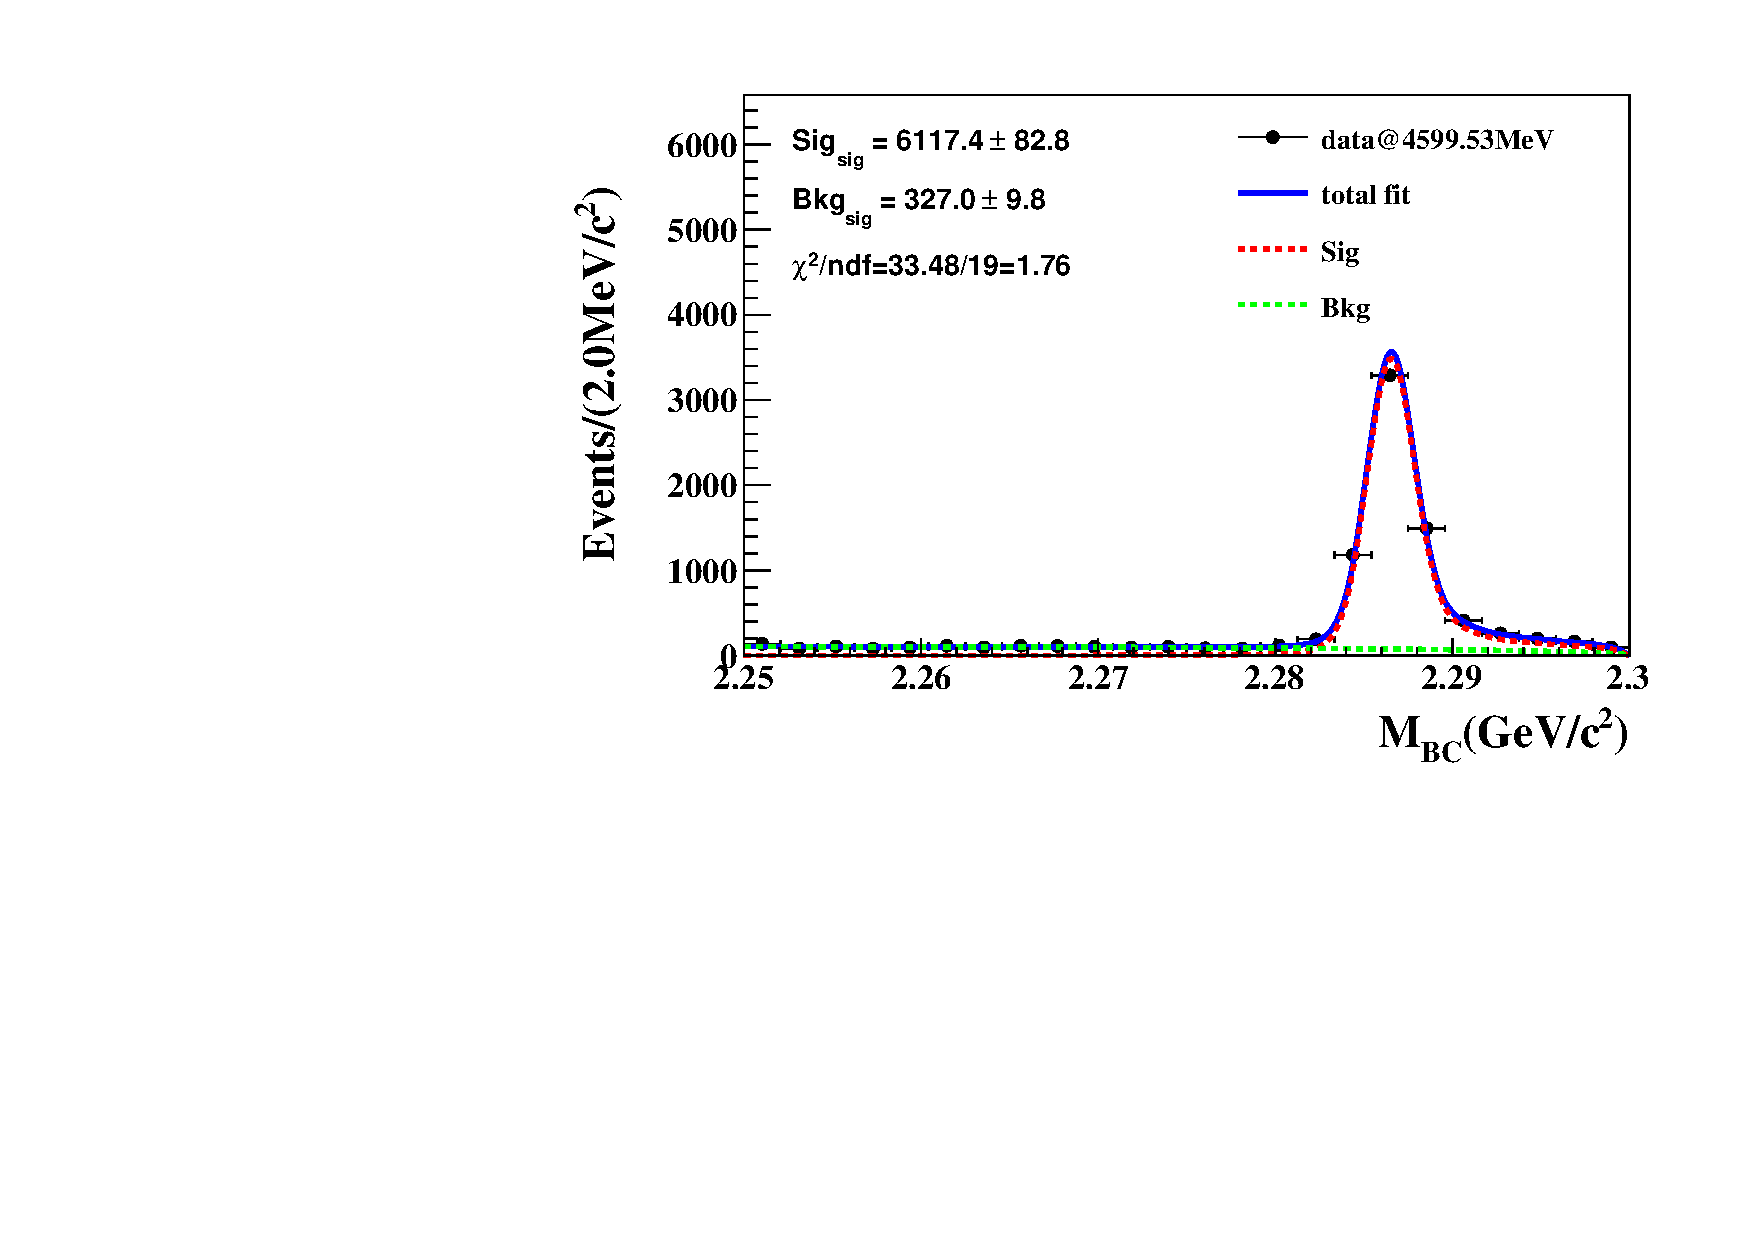
\includegraphics[width=0.32\textwidth]{figure/fit_mbc/STdata4600_1001.pdf}
    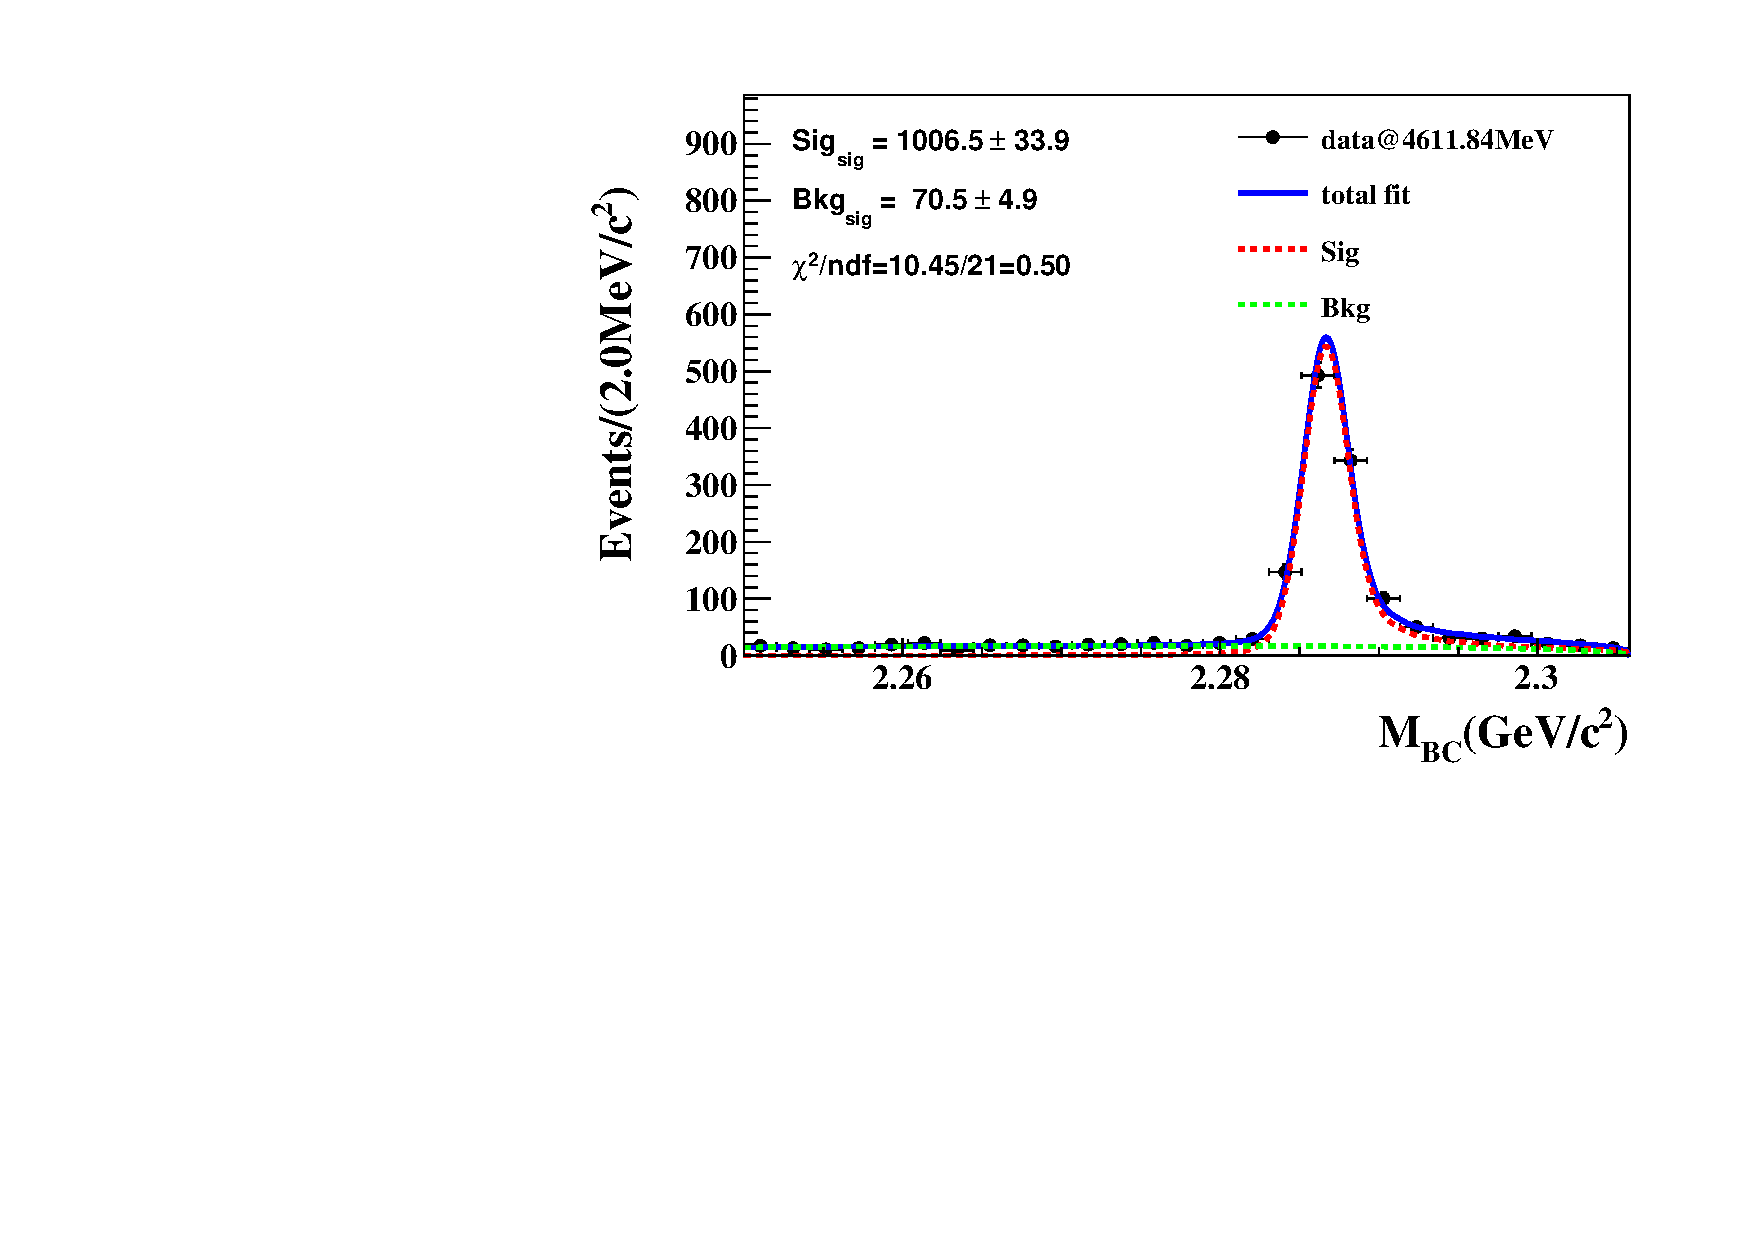
\includegraphics[width=0.32\textwidth]{figure/fit_mbc/STdata4612_1001.pdf}
    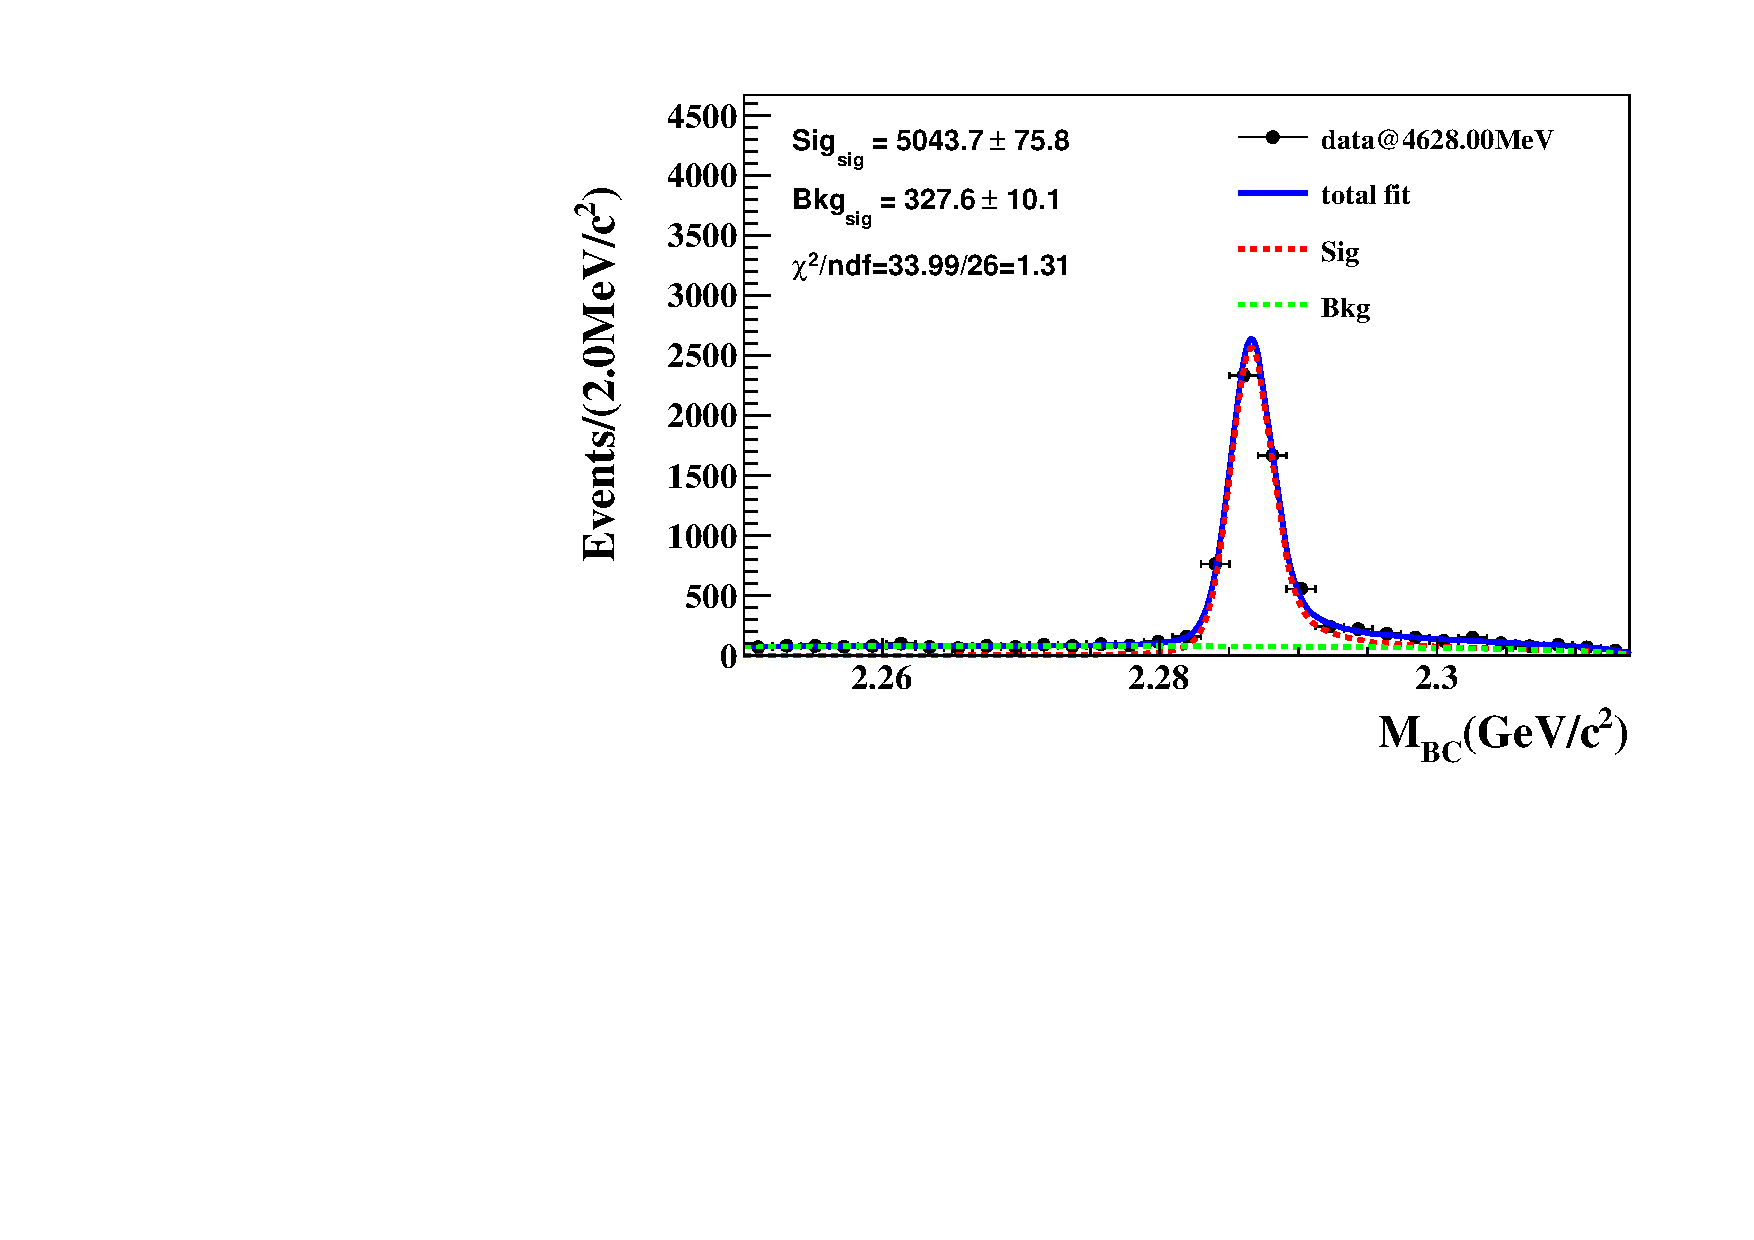
\includegraphics[width=0.32\textwidth]{figure/fit_mbc/STdata4626_1001.pdf}\\
    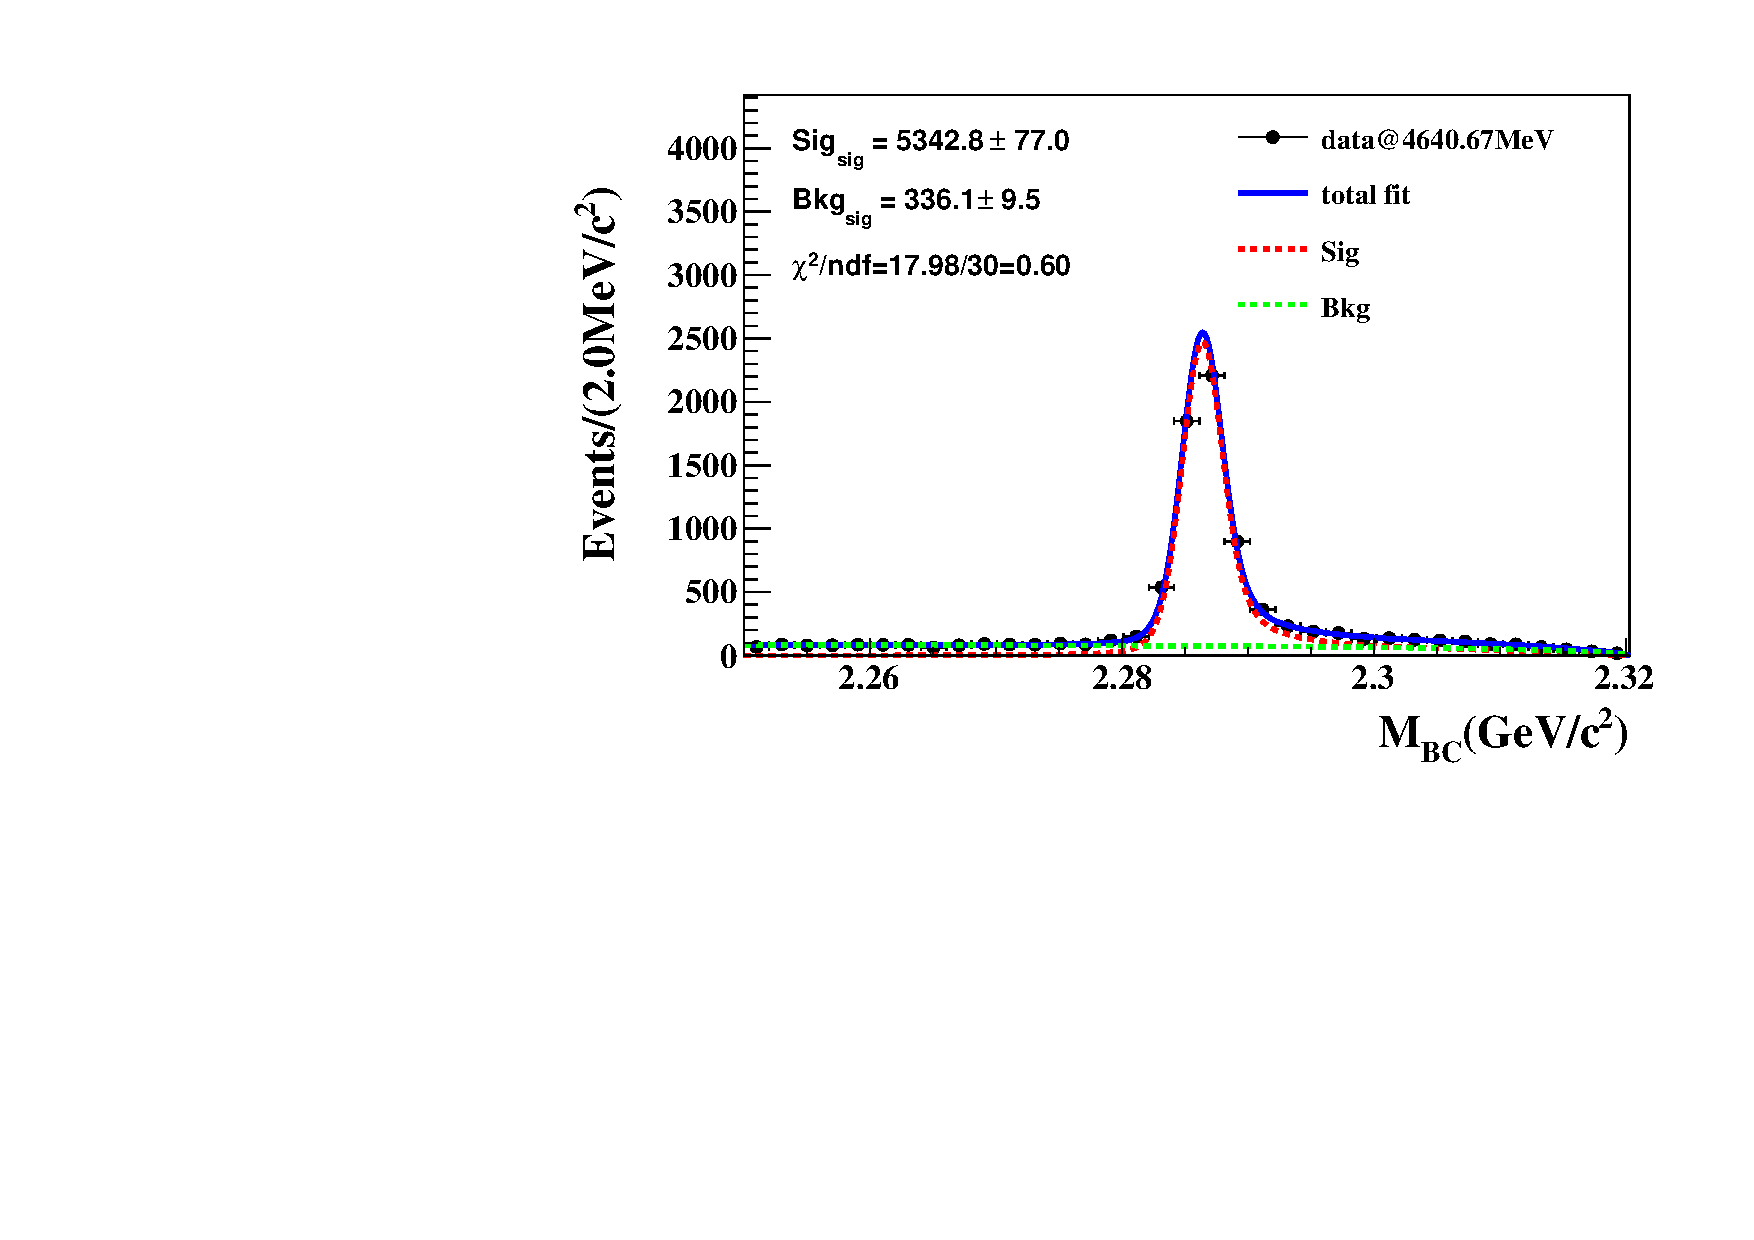
\includegraphics[width=0.32\textwidth]{figure/fit_mbc/STdata4640_1001.pdf}
    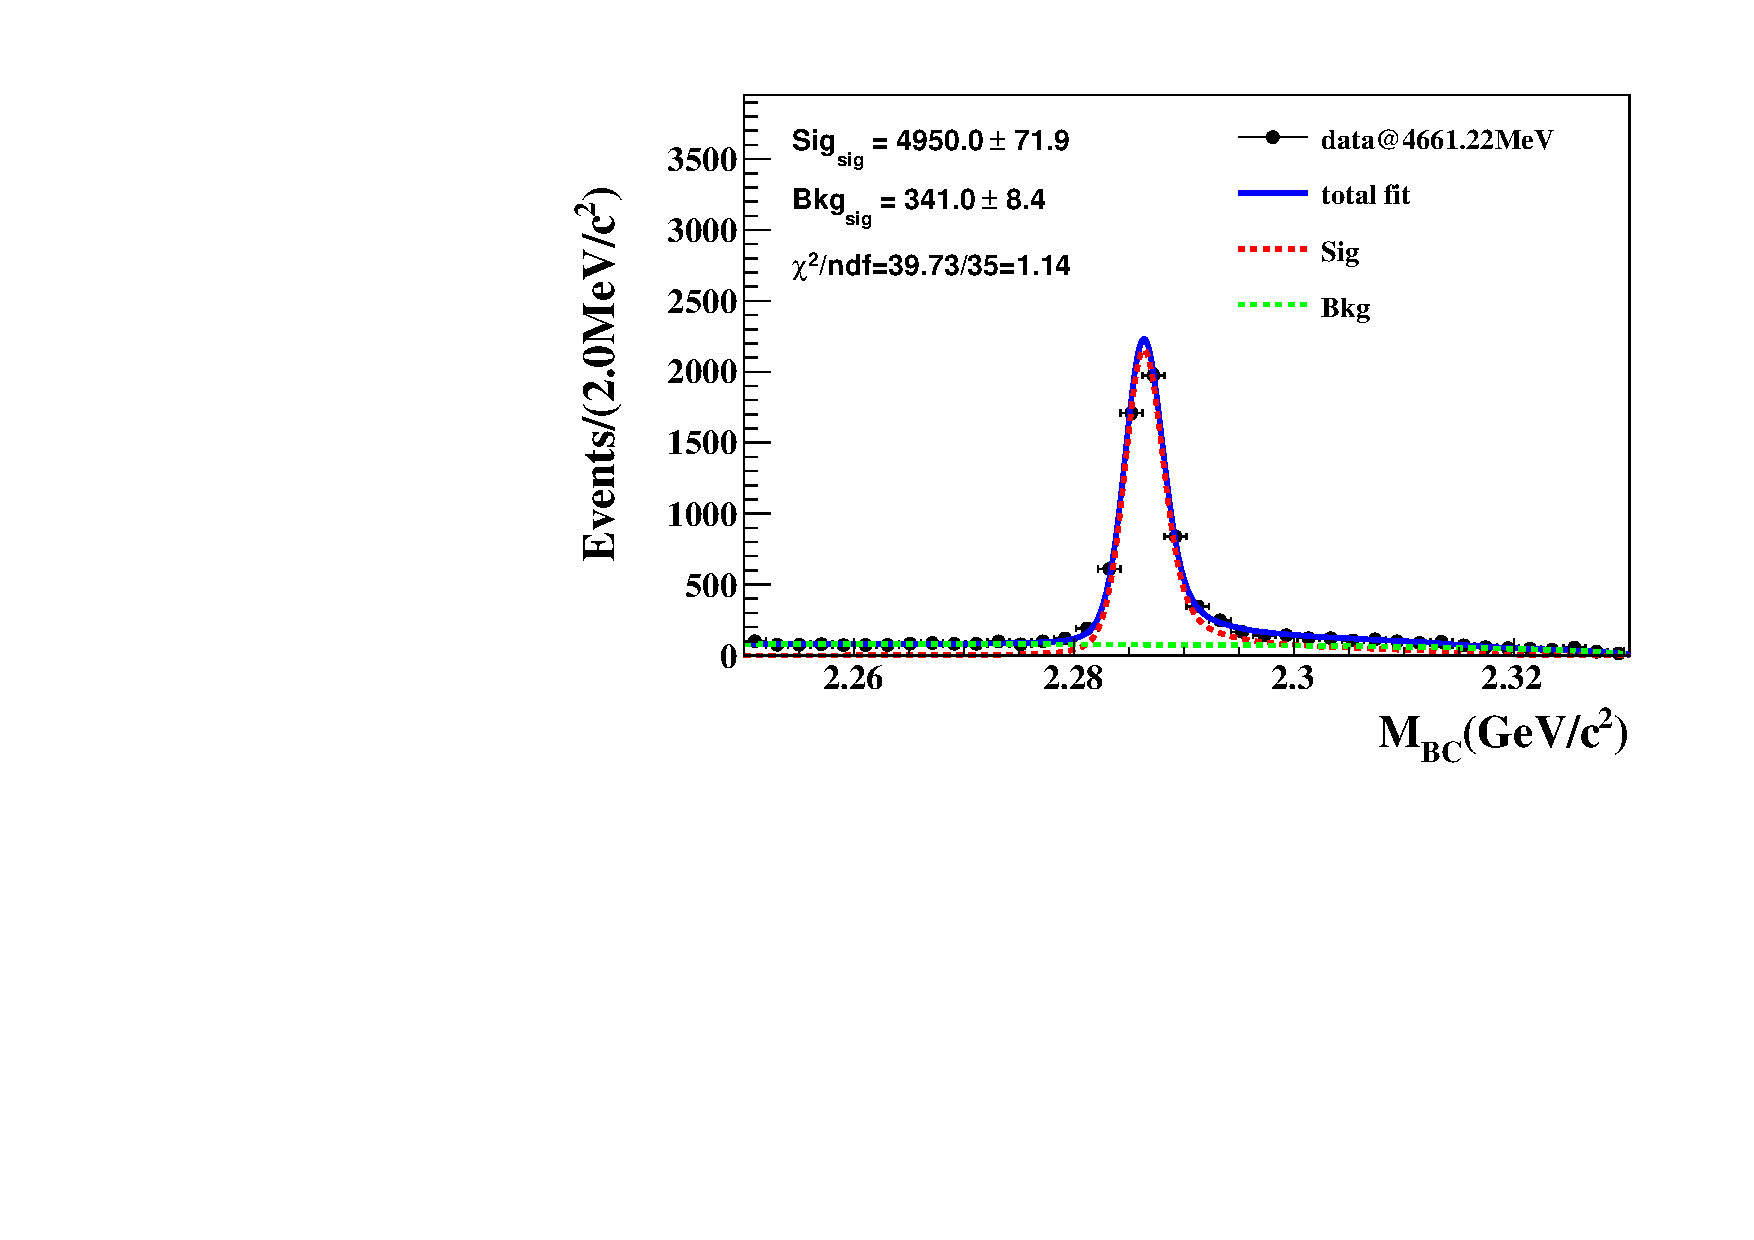
\includegraphics[width=0.32\textwidth]{figure/fit_mbc/STdata4660_1001.pdf}
    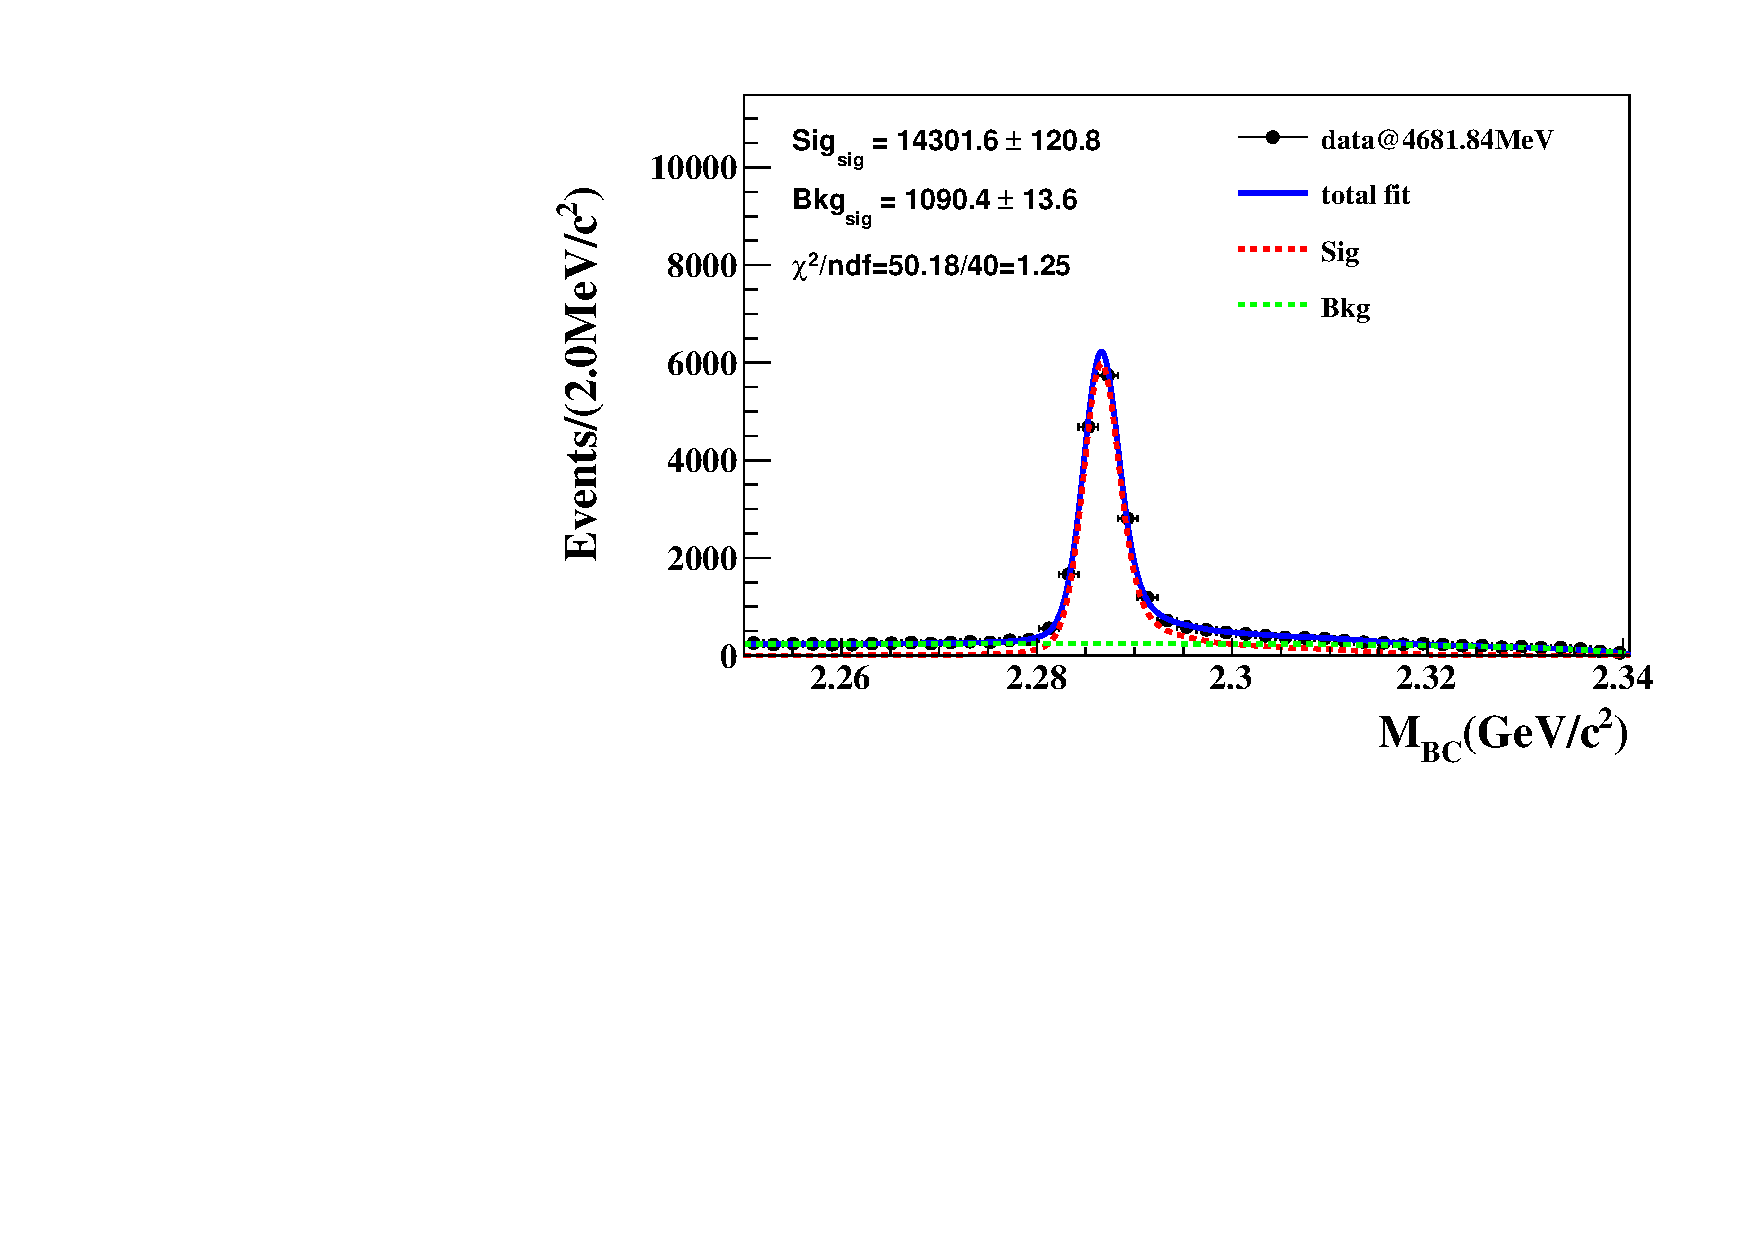
\includegraphics[width=0.32\textwidth]{figure/fit_mbc/STdata4680_1001.pdf}\\
    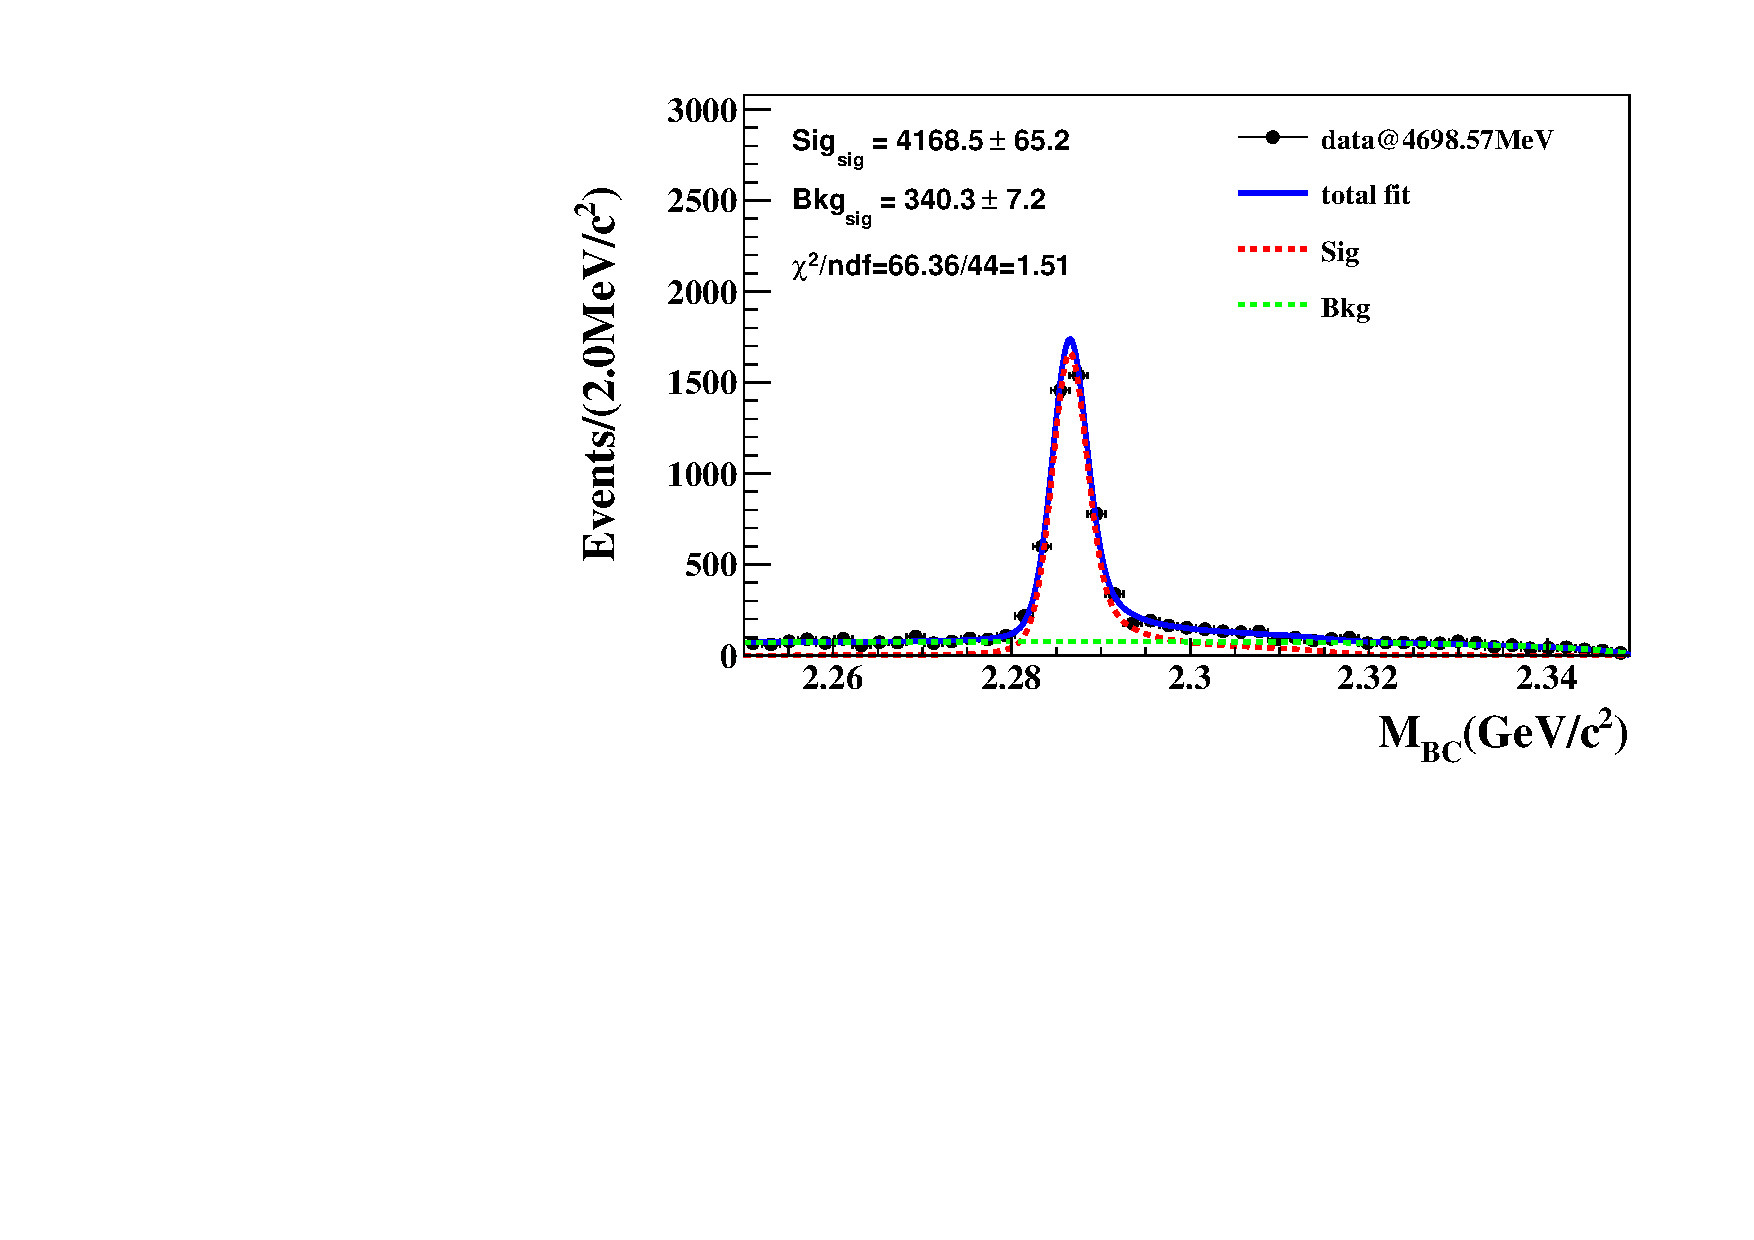
\includegraphics[width=0.32\textwidth]{figure/fit_mbc/STdata4700_1001.pdf}
    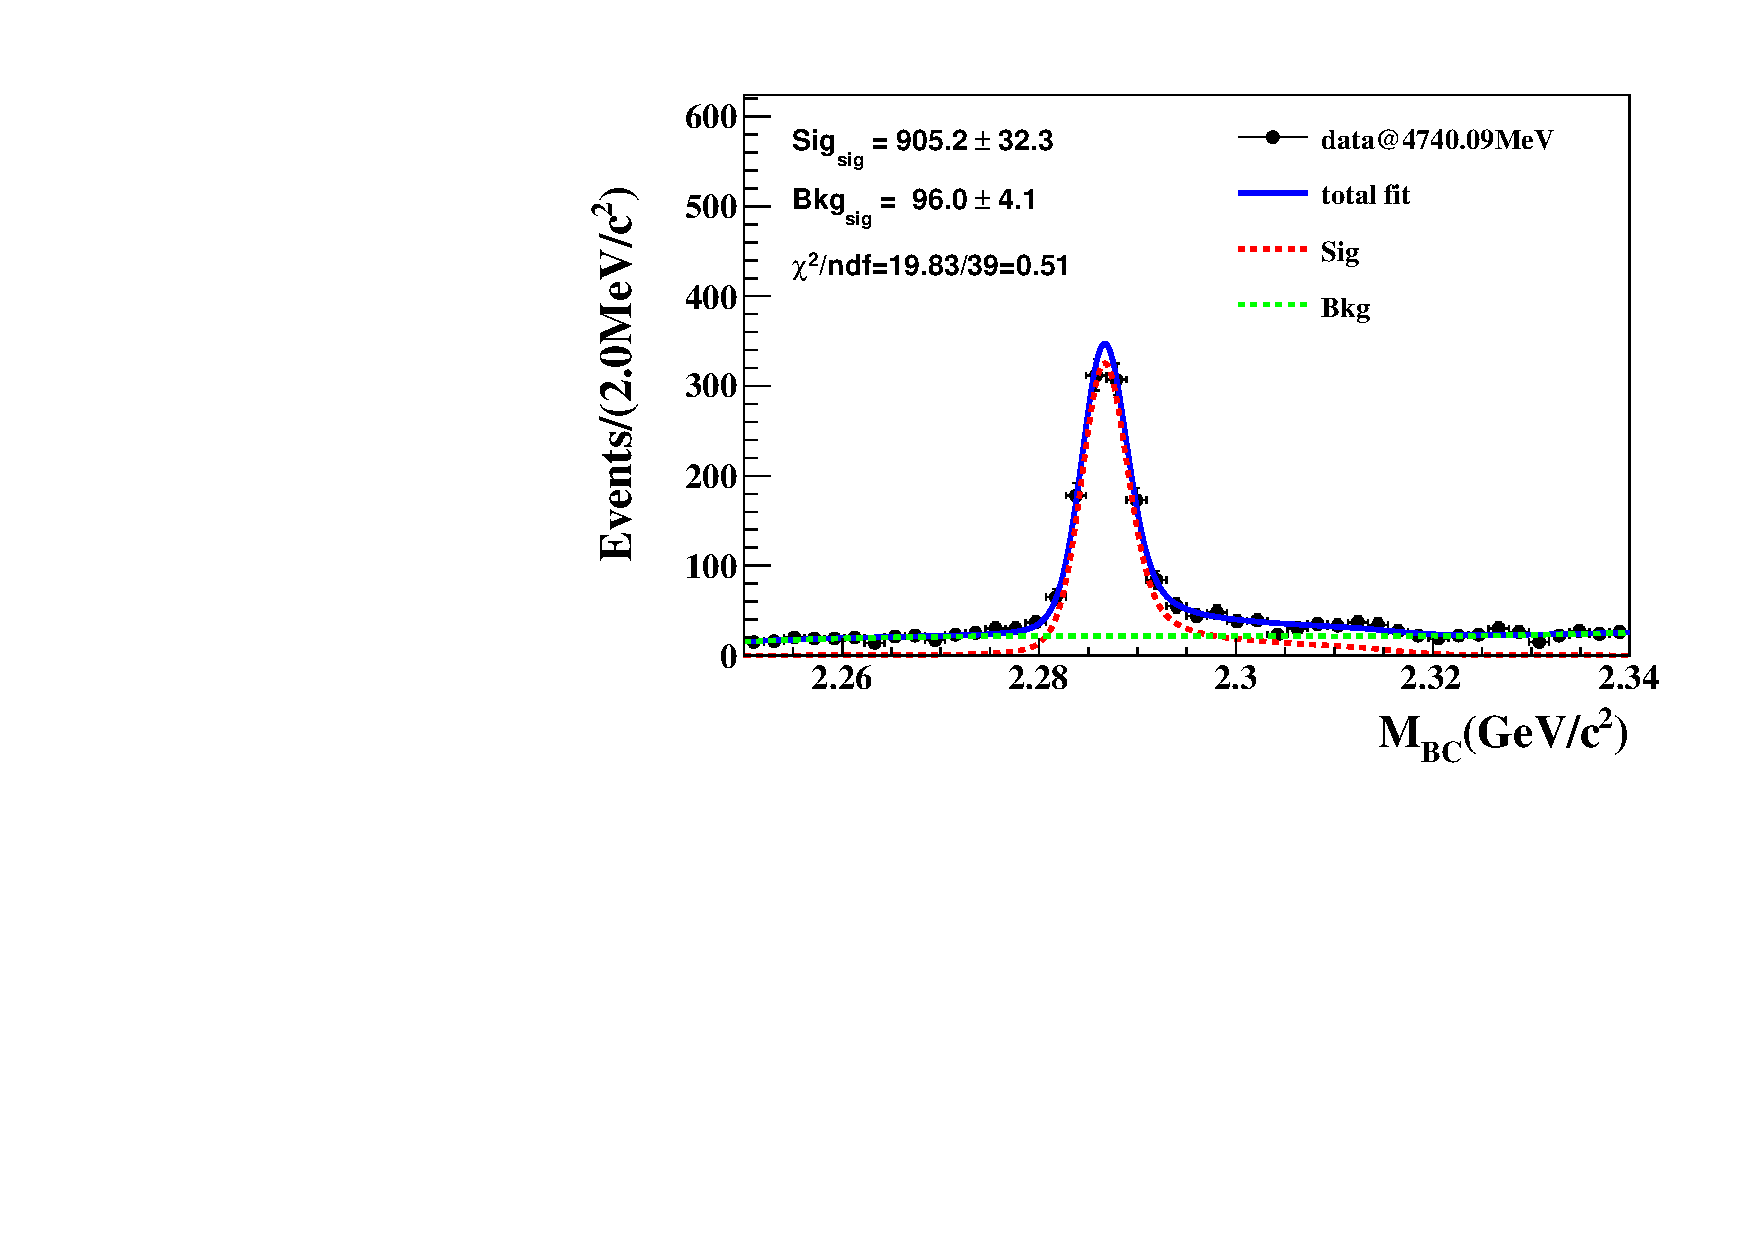
\includegraphics[width=0.32\textwidth]{figure/fit_mbc/STdata4740_1001.pdf}
    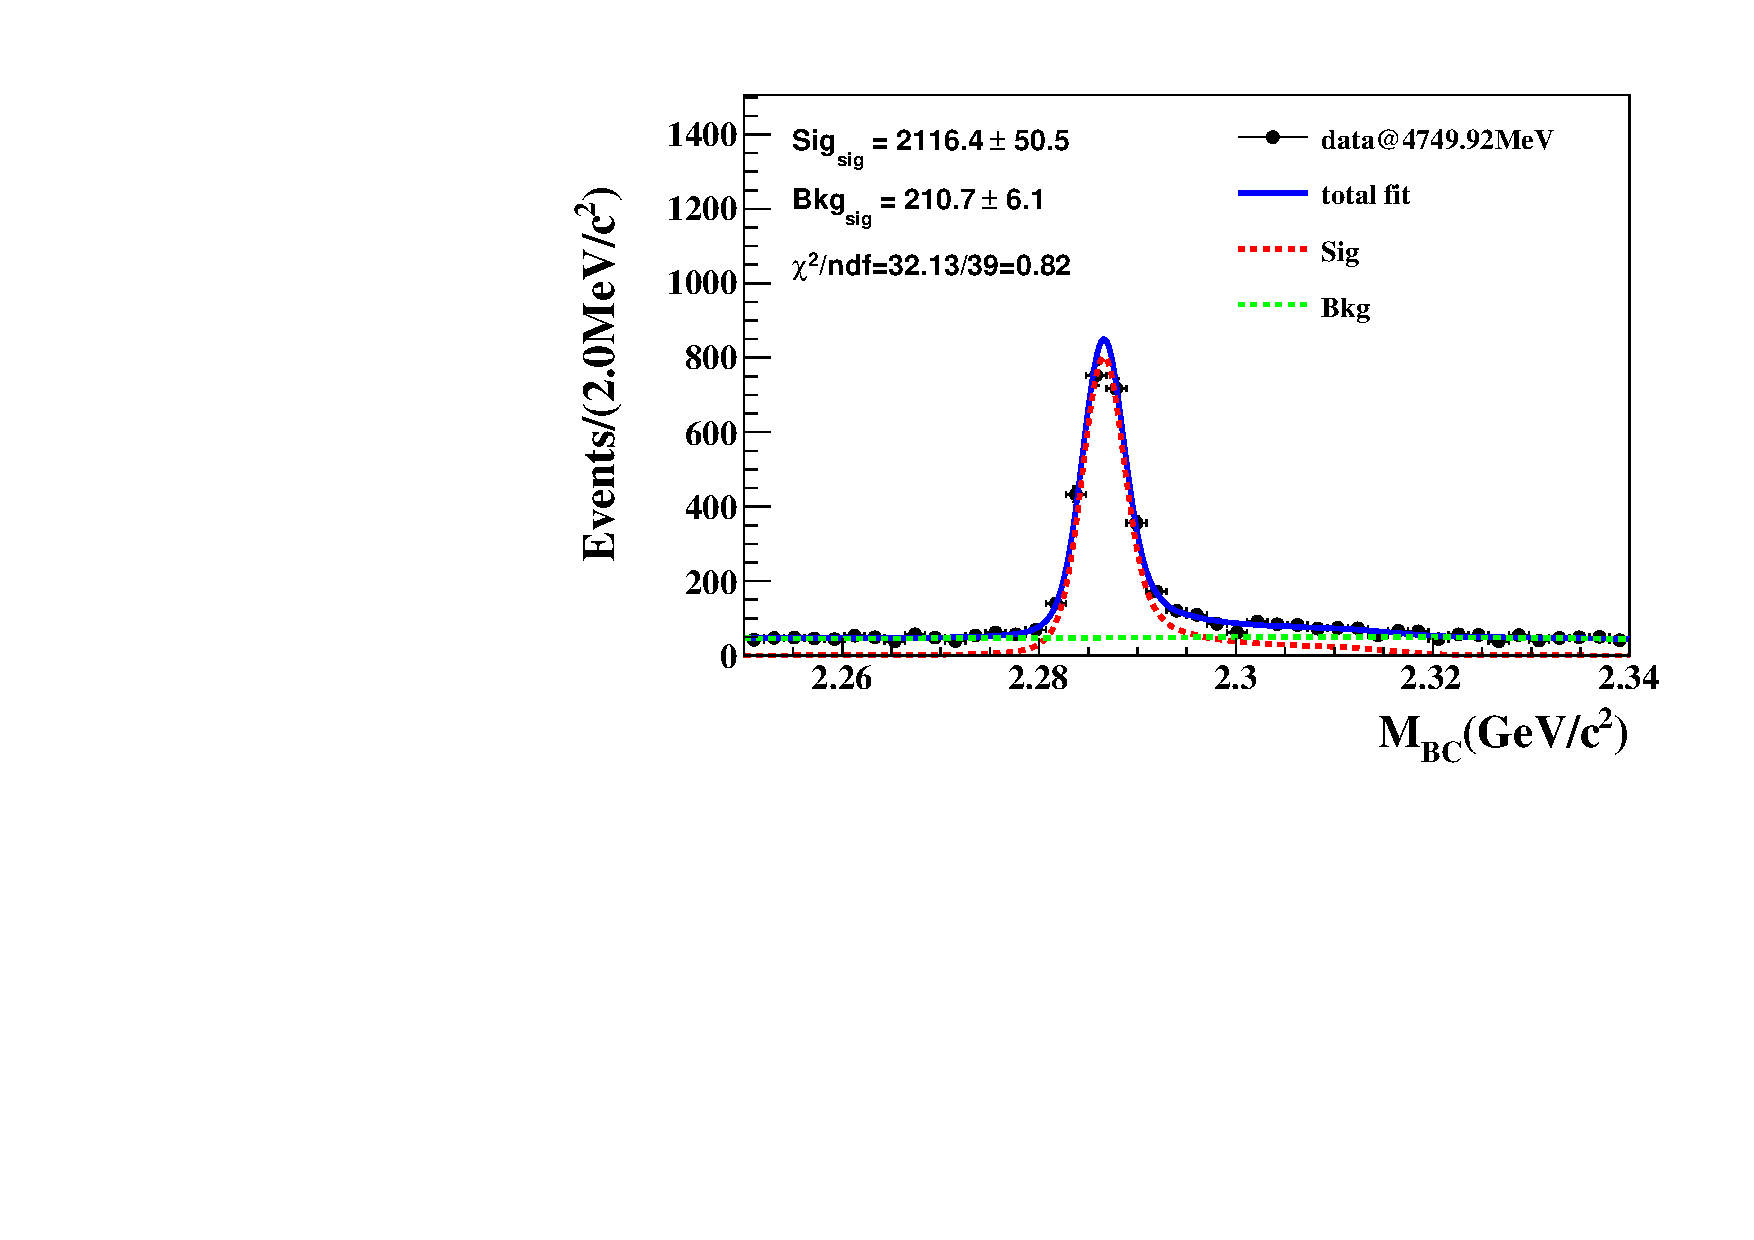
\includegraphics[width=0.32\textwidth]{figure/fit_mbc/STdata4750_1001.pdf}\\
    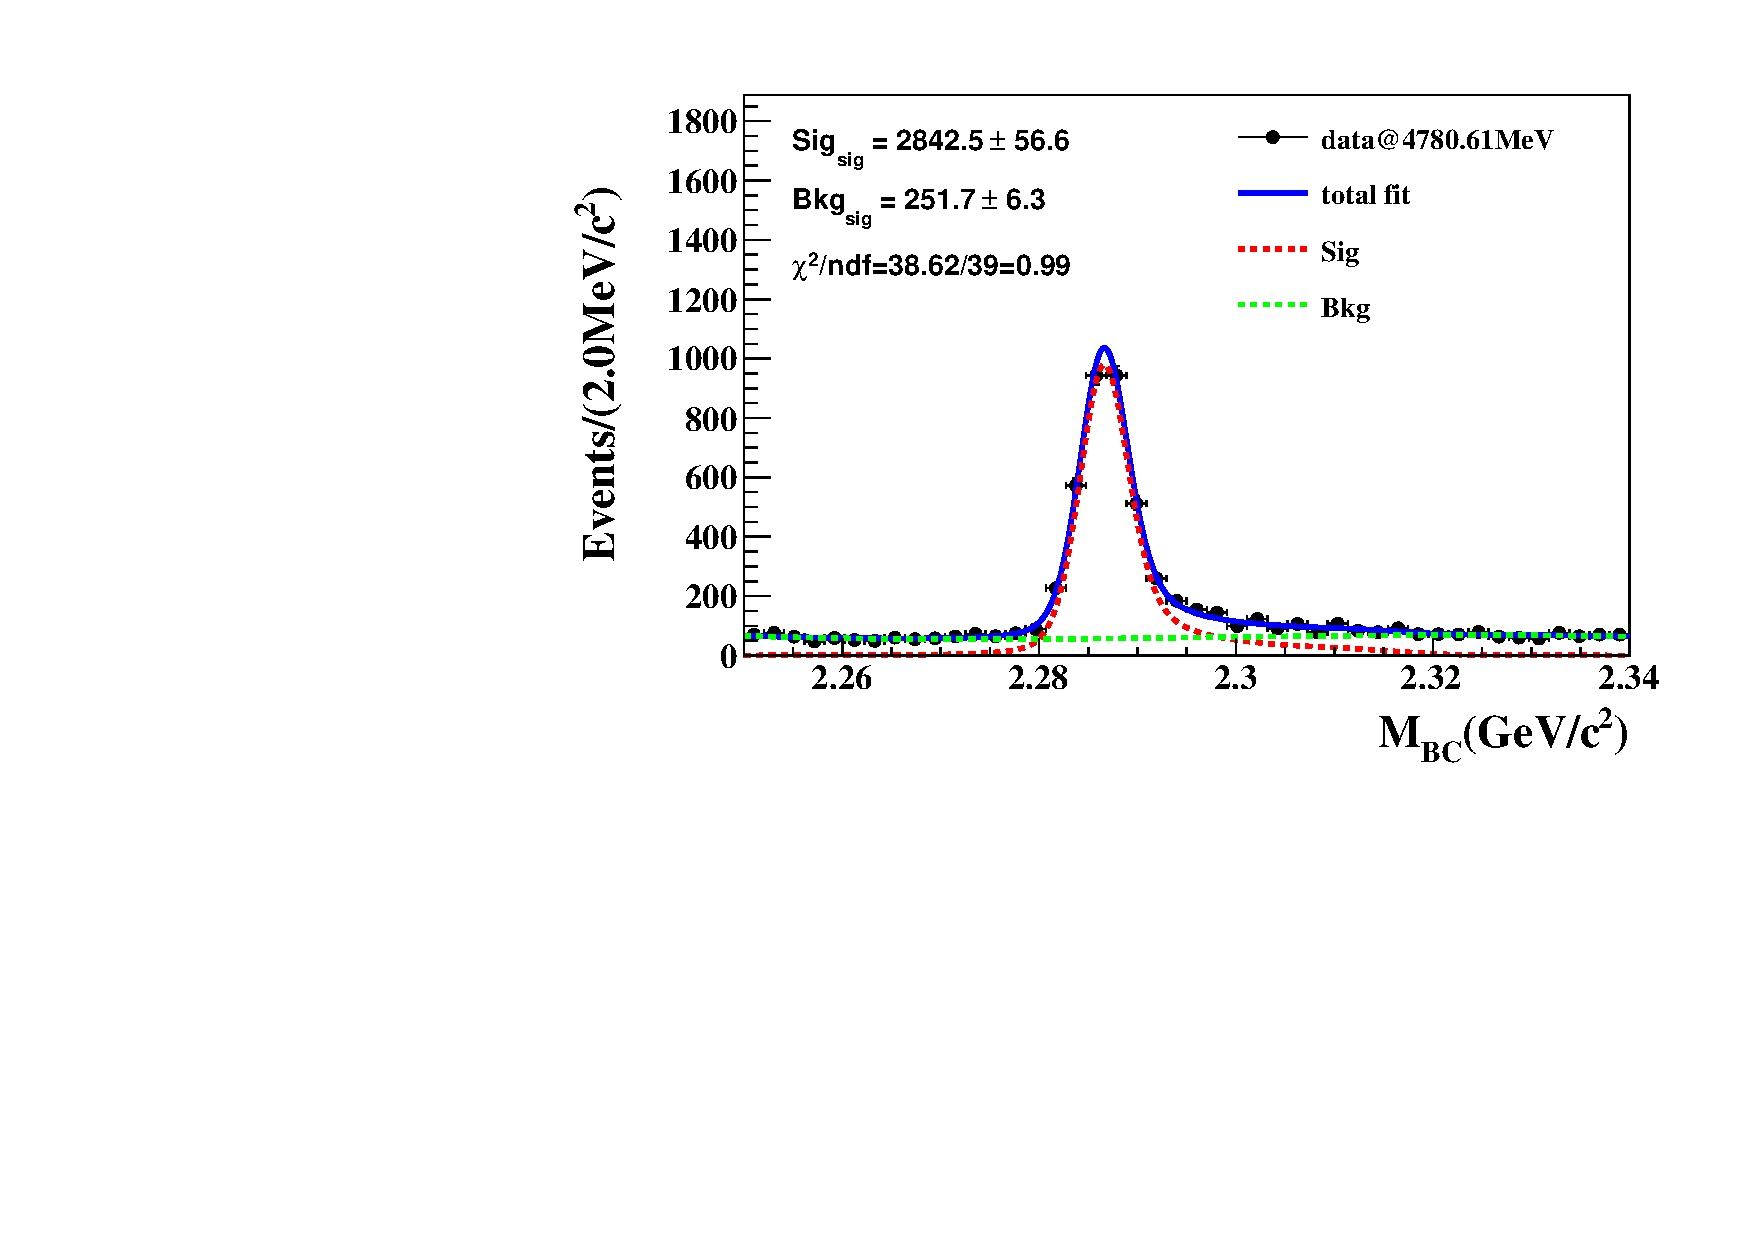
\includegraphics[width=0.32\textwidth]{figure/fit_mbc/STdata4780_1001.pdf}
    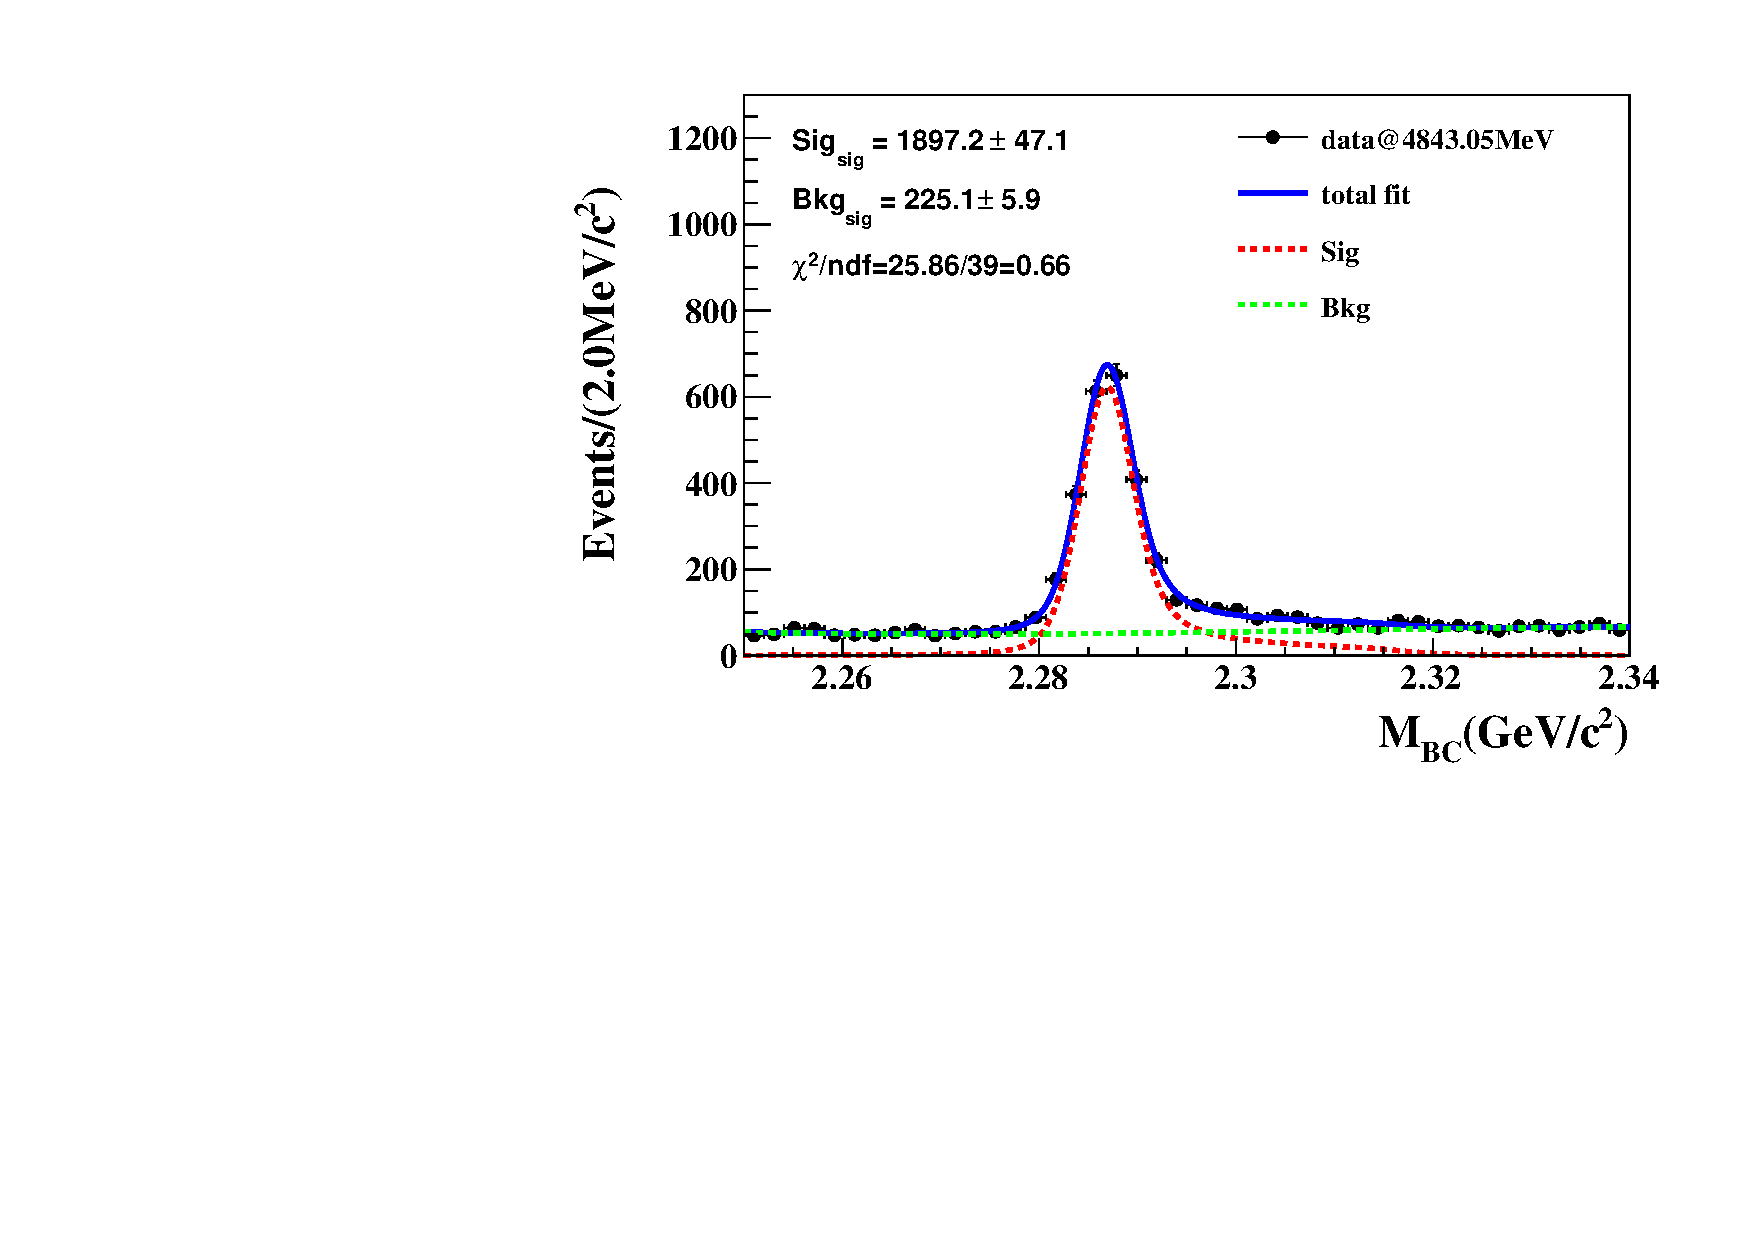
\includegraphics[width=0.32\textwidth]{figure/fit_mbc/STdata4840_1001.pdf}
    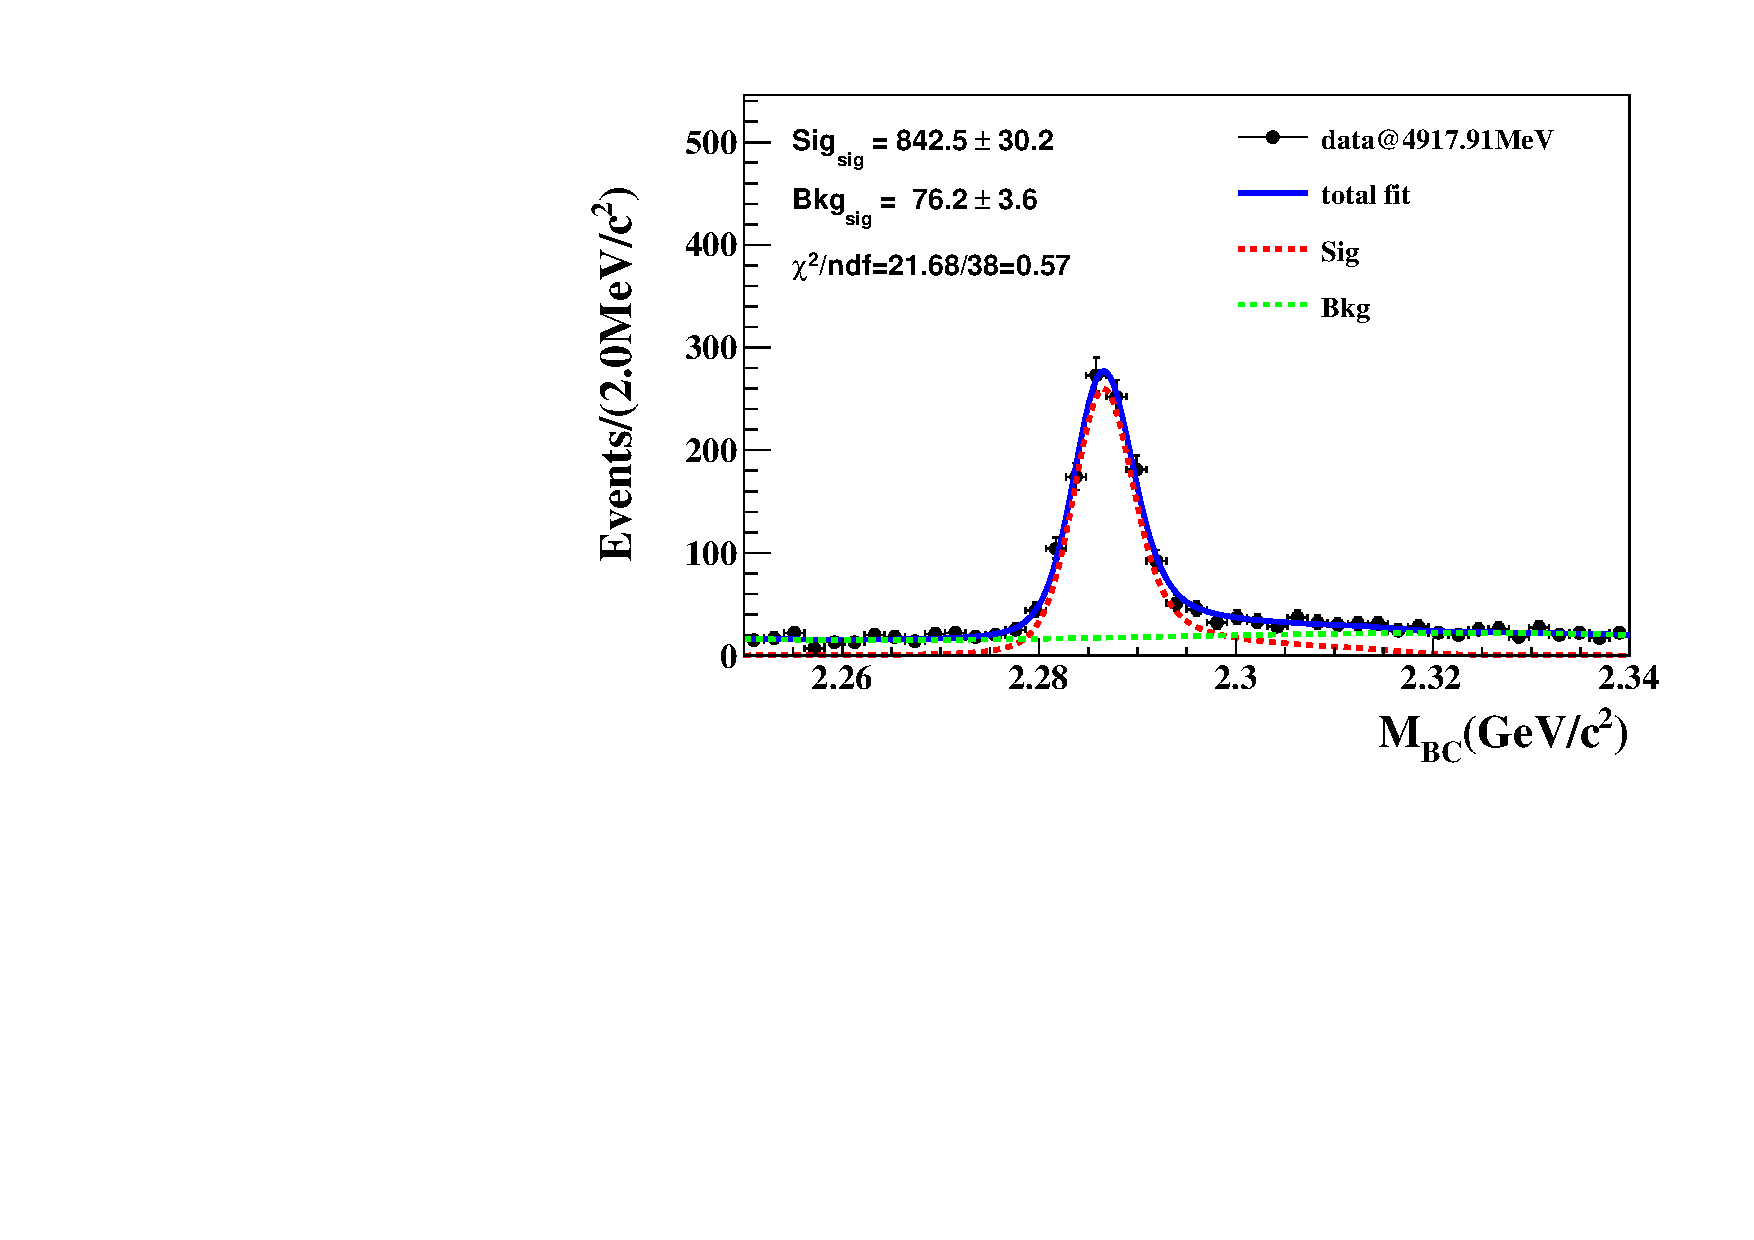
\includegraphics[width=0.32\textwidth]{figure/fit_mbc/STdata4914_1001.pdf}\\
    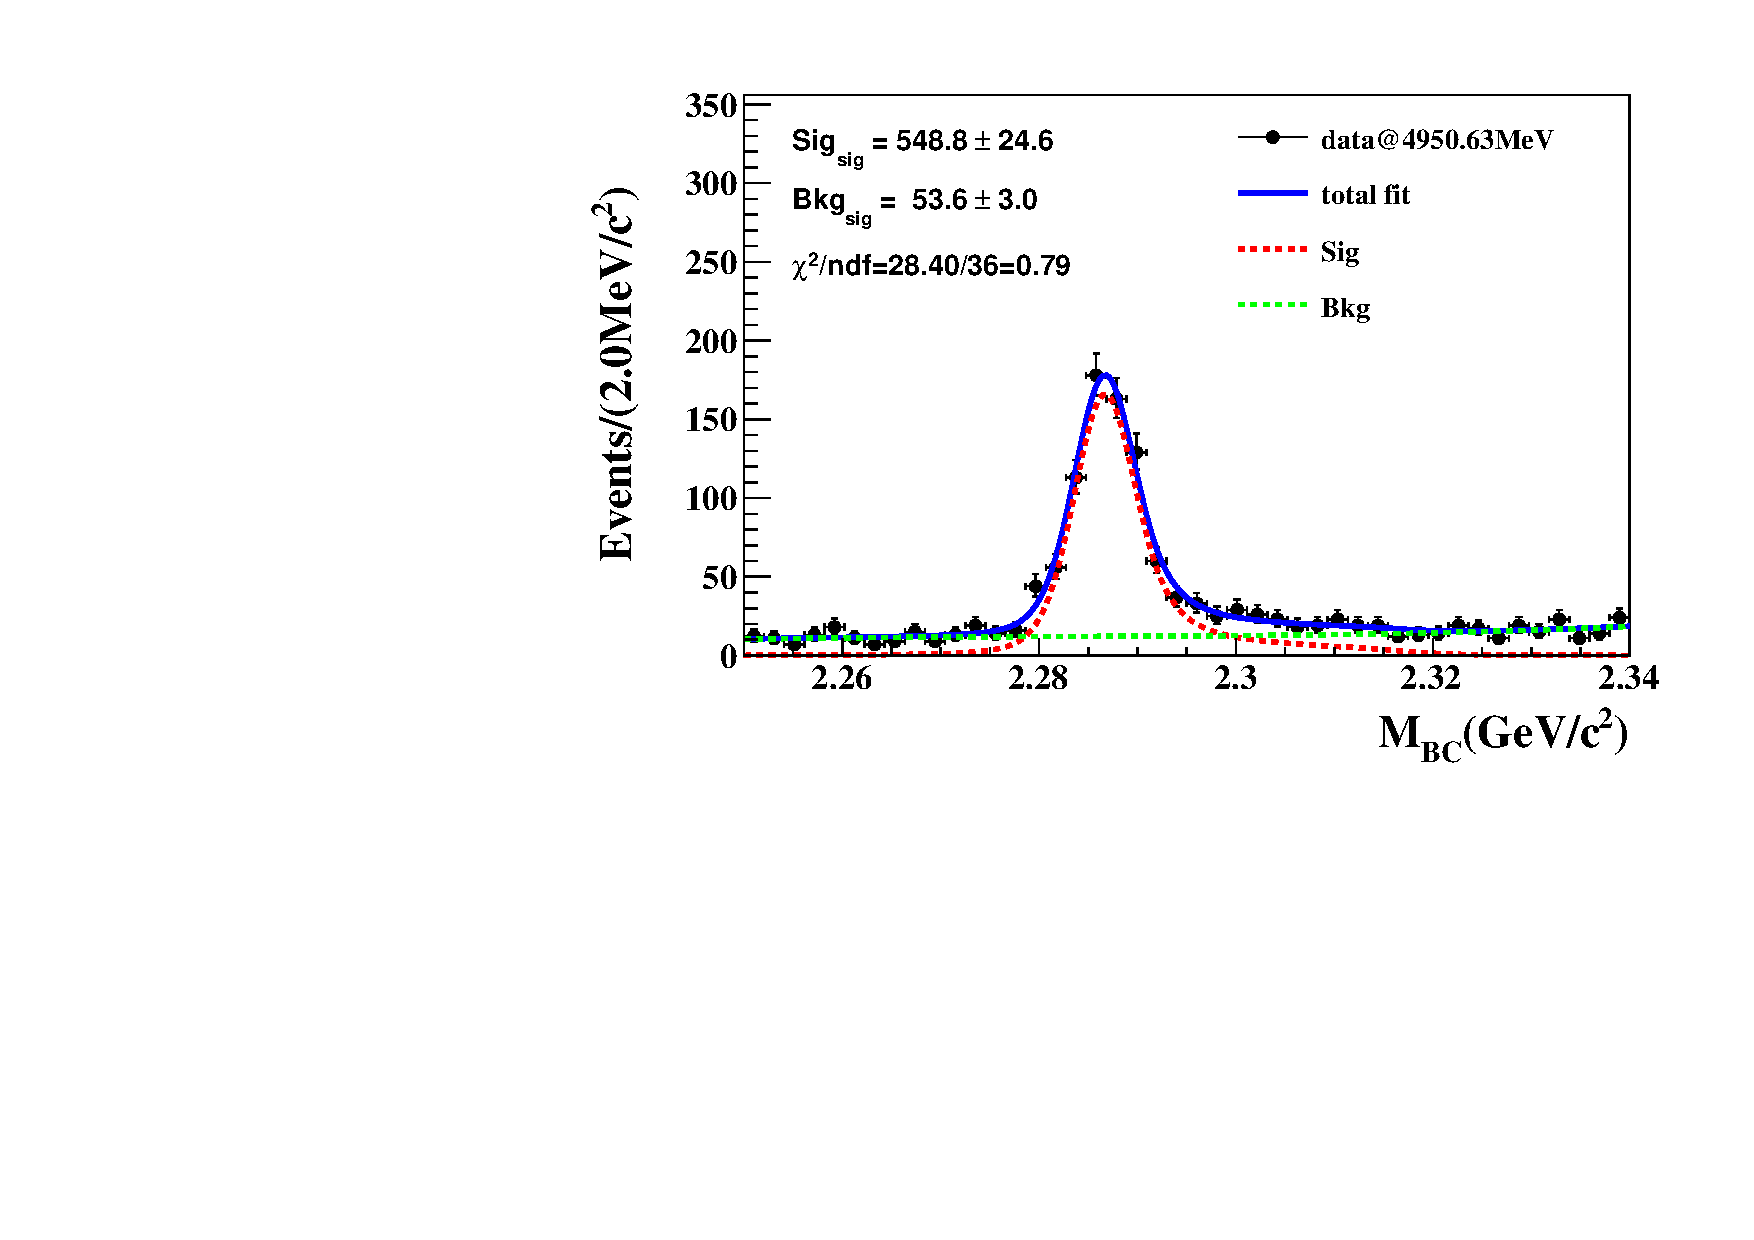
\includegraphics[width=0.32\textwidth]{figure/fit_mbc/STdata4946_1001.pdf}
    \caption{Fit results on $\mbc$ distributions for each energy point.}
\label{fig:fit_mbc}
\end{figure}

\begin{table}\centering
    \caption{Fit results within signal regions for each energy point, with $\mbc$ requirements, signal yields, background yields, signal purities, background fractions and convolved Gaussian width values. }
    \label{tab:fit_mbc_results}
    \resizebox{\textwidth}{!}{
    \begin{tabular}{ccccccc}
        \hline\hline
     & Signal region(GeV/$c^2$) & Signal yields & Bkg yields & Signal purity (\%) & Bkg fraction (\%) & Gaussian width (MeV/$c^2$)\\\hline
     4600 & [2.282, 2.291] & 6117$\pm$83 & 327$\pm$10 & 94.9$\pm$0.2 & 5.1$\pm$0.2 & 0.16$\pm$0.06\\
     4612 & [2.282, 2.291] & 1006$\pm$34 & 70$\pm$5 & 93.5$\pm$0.5 & 6.5$\pm$0.5 & 0.03$\pm$0.17\\
     4626 & [2.282, 2.291] & 5044$\pm$76 & 328$\pm$10 & 93.9$\pm$0.2 & 6.1$\pm$0.2 & 0.14$\pm$0.15\\
     4640 & [2.282, 2.291] & 5343$\pm$77 & 336$\pm$10 & 94.1$\pm$0.2 & 5.9$\pm$0.2 & 0.39$\pm$0.11\\
     4660 & [2.282, 2.291] & 4950$\pm$72 & 341$\pm$8 & 93.6$\pm$0.2 & 6.4$\pm$0.2 & 0.44$\pm$0.11\\
     4680 & [2.282, 2.291] & 14302$\pm$121 & 1090$\pm$14 & 92.9$\pm$0.1 & 7.1$\pm$0.1 & 0.46$\pm$0.07\\
     4700 & [2.282, 2.291] & 4168$\pm$65 & 340$\pm$7 & 92.5$\pm$0.2 & 7.5$\pm$0.2 & 0.57$\pm$0.12\\
     4740 & [2.282, 2.291] & 906$\pm$33 & 97$\pm$4 & 90.3$\pm$0.6 & 9.7$\pm$0.6 & 0.87$\pm$0.24\\
     4750 & [2.282, 2.291] & 2116$\pm$51 & 211$\pm$6 & 90.9$\pm$0.4 & 9.1$\pm$0.4 & 0.42$\pm$0.27\\
     4780 & [2.282, 2.291] & 2846$\pm$58 & 255$\pm$7 & 91.8$\pm$0.3 & 8.2$\pm$0.3 & 0.88$\pm$0.15\\
     4840 & [2.282, 2.291] & 1900$\pm$49 & 229$\pm$6 & 89.3$\pm$0.4 & 10.7$\pm$0.4 & 0.79$\pm$0.24\\
     4920 & [2.282, 2.291] & 844$\pm$31 & 77$\pm$4 & 91.7$\pm$0.6 & 8.3$\pm$0.6 & 0.92$\pm$0.36\\
     4950 & [2.282, 2.291] & 553$\pm$25 & 56$\pm$3 & 90.8$\pm$0.7 & 9.2$\pm$0.7 & 0.05$\pm$2.89\\
    \hline\hline
    \end{tabular}
    }
\end{table}

\subsection{Check of sideband regions}
\label{sec:sideband_check}

After applying all selection criteria, an additional kinematic fit is performed to improve the momentum resolution of particles for the amplitude analysis. The kinematic constraints are listed below:
\begin{itemize}
    \item Signal side $\lcp$, reconstructed by $p$, $K^-$ and $\pi^+$ is constrained at the $\Lambda_c$ nominal mass value,
    \item Recoil side $\lcm$ is constrained at the $\Lambda_c$ nominal mass value using information of initial four-momentum of $e^+e^-$ collision.
\end{itemize}
No cut is applied on the fit quality of the kinematic fit.

In the amplitude analysis, the background contributions are modeled by the data events in the $\mbc$ sideband region, scaled according to the background fractions from the $\mbc$ fit. It is crucial to valid the consistency of the background shape between the $\mbc$ sideband region and signal region. Shapes of $M^2(pK^-)$, $M^2(p\pi^+)$ and $M^2(K^-\pi^+)$ are compared using the data events and cocktail MC samples with signal process vetoed. Figure~\ref{fig:comp_mc_sideband} shows the shape comparison for cocktail MC samples in the $\mbc$ signal and sideband regions. The distributions of $M^2(pK^-)$ and $M^2(p\pi^+)$ in the $\mbc$ signal and sideband regions agree well with each other within uncertainties. Discrepancy is observed in the distribution of $M^2(K^-\pi^+)$. 
Figure~\ref{fig:comp_datamc_sideband} shows the comparison results between data and cocktail MC in the $\mbc$ sideband region. Visible difference can be observed in the distribution of $M^2(K^-\pi^+)$, which arises from the lack of modelling on $\bar{K}^*$ processes in the cocktail MC samples. In the nominal amplitude analysis, we still trust data and use data events in $\mbc$ sideband region to describe the background. The observed disagreements in the Figure~\ref{fig:comp_mc_sideband}, \ref{fig:comp_datamc_sideband} will be considered for possible variations of the background shape in the study of systematic uncertainties. More details about the source of background are documented in Appendix~\ref{app:bkg_check}.

\begin{figure}[H]\centering
    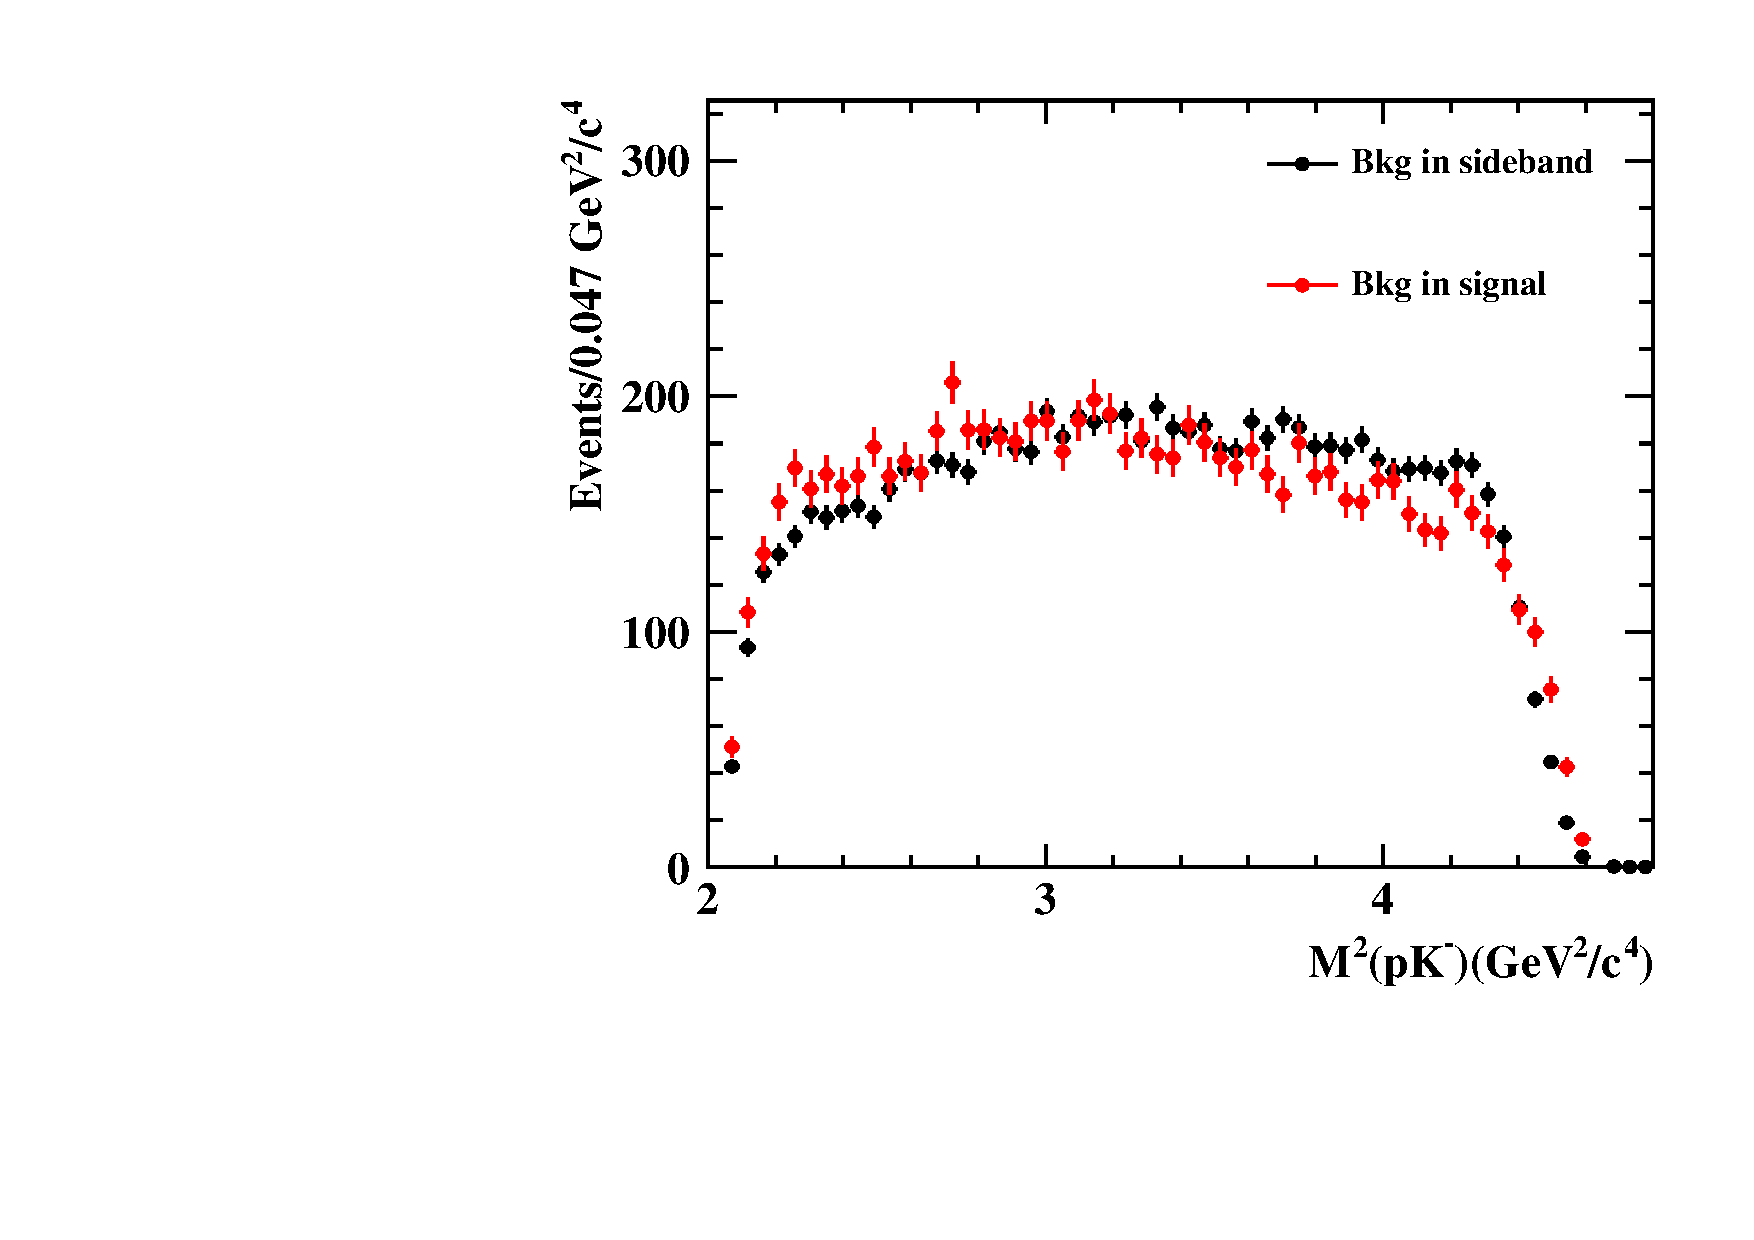
\includegraphics[width=0.325\textwidth]{figure/sideband/output_mc_0_sideband_signal_m2_12_2c_1.pdf}
    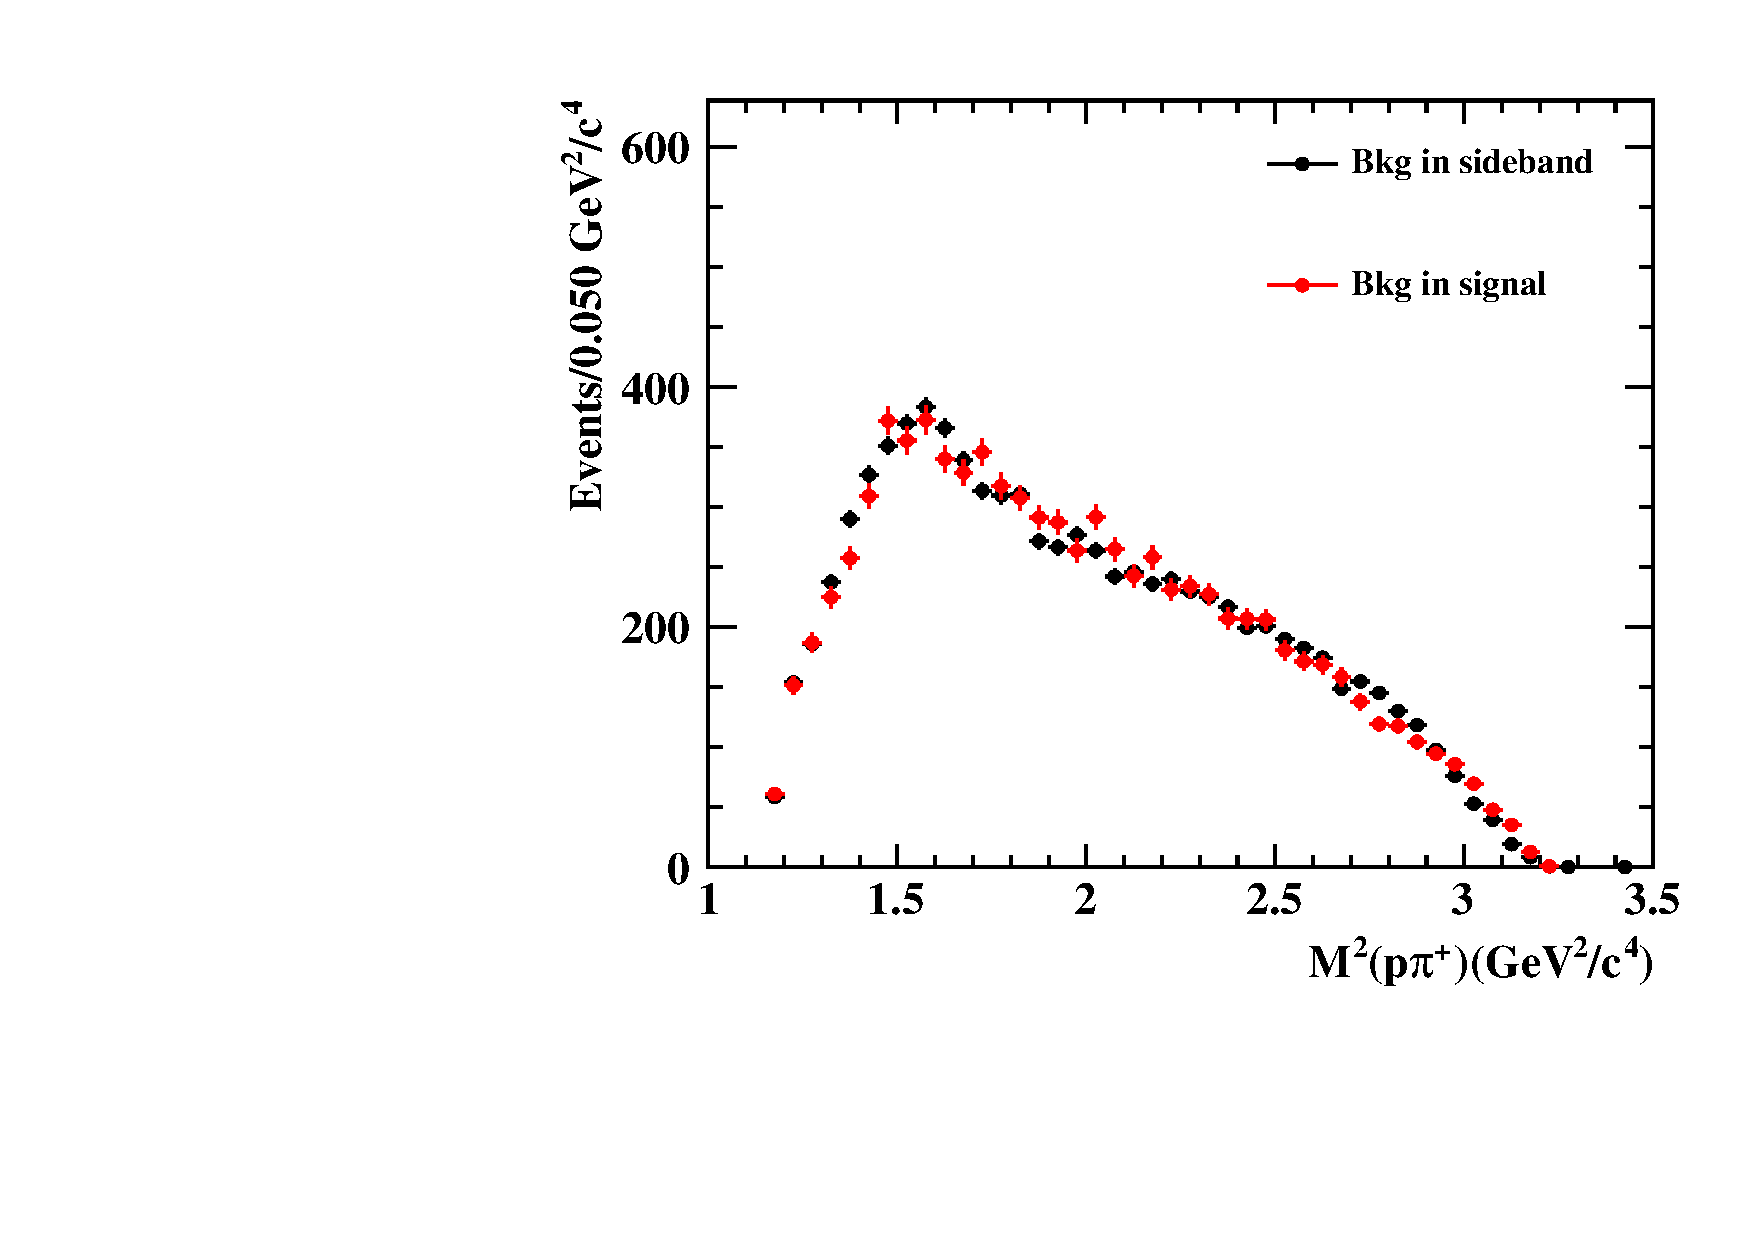
\includegraphics[width=0.325\textwidth]{figure/sideband/output_mc_0_sideband_signal_m2_13_2c_1.pdf}
    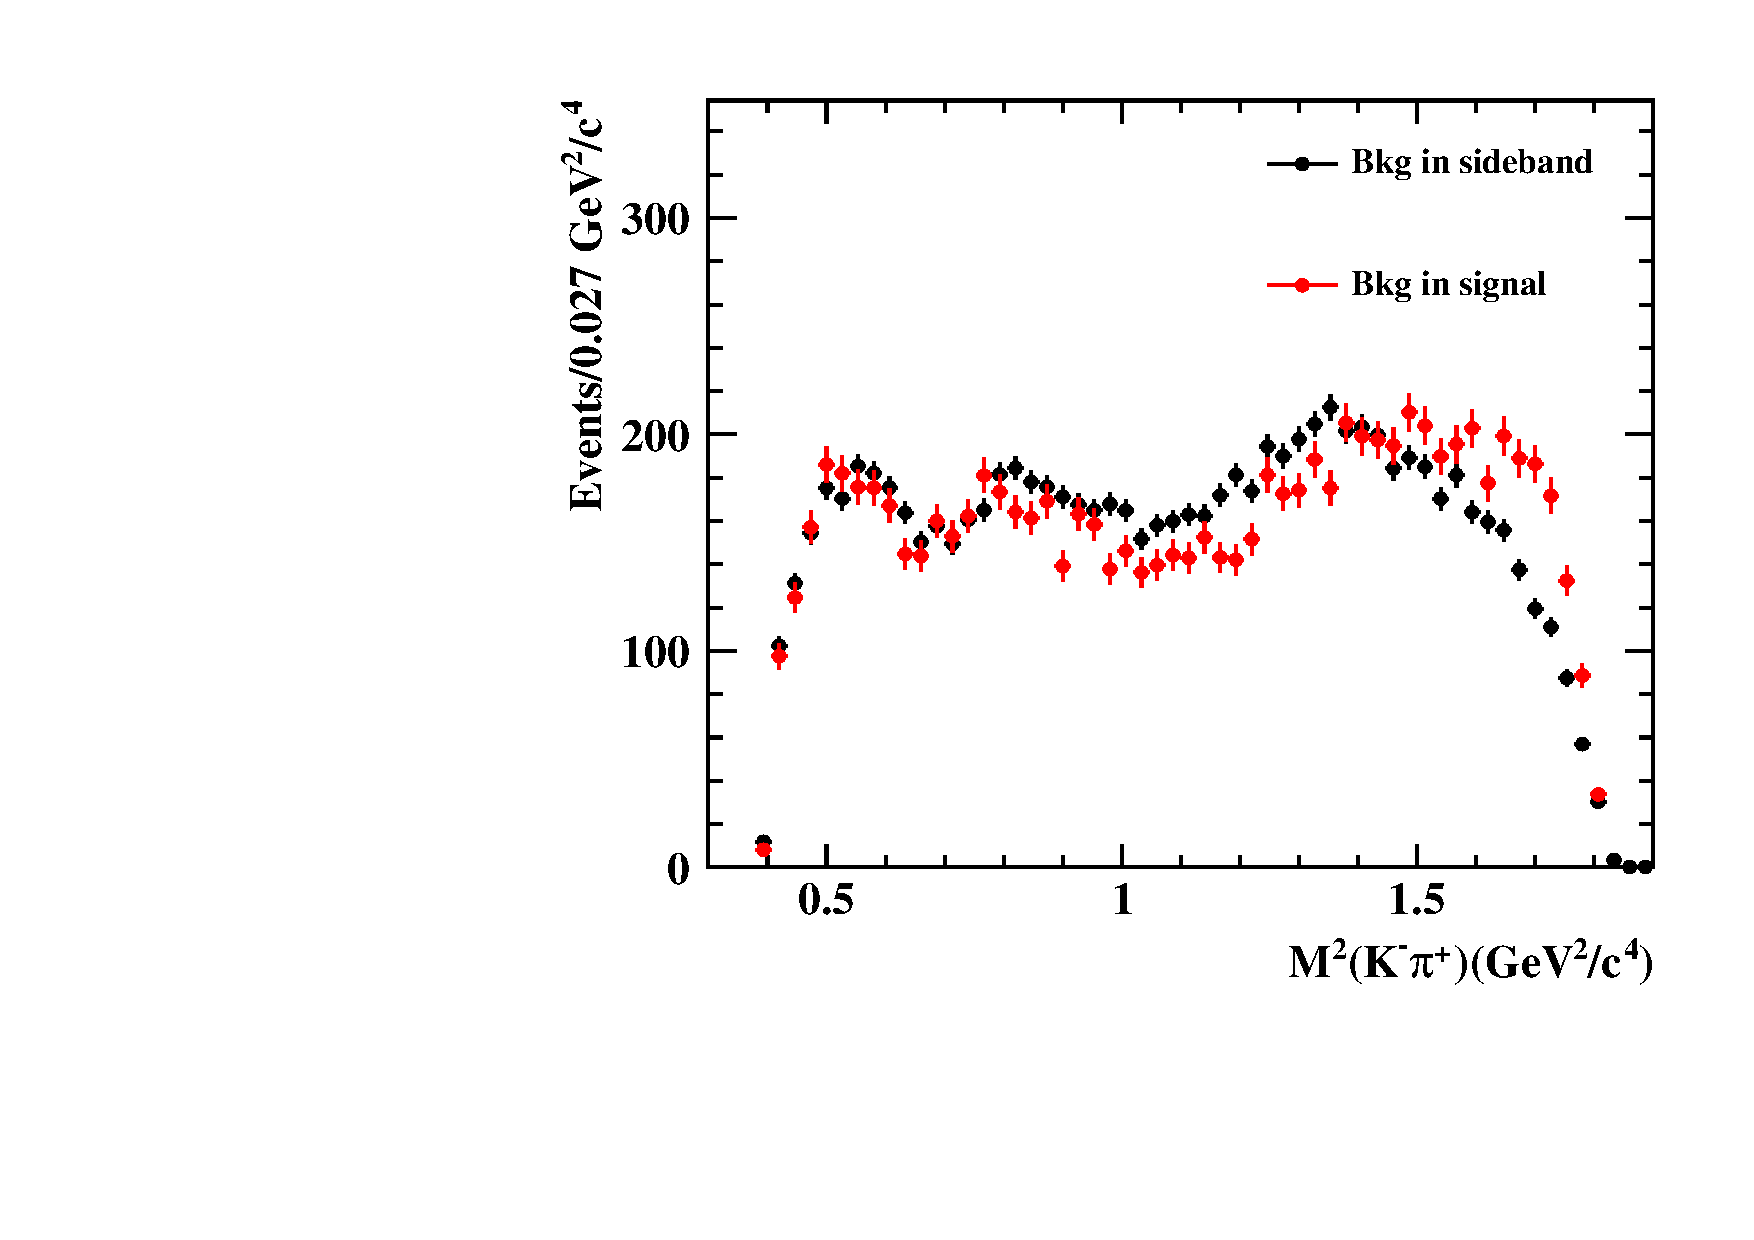
\includegraphics[width=0.325\textwidth]{figure/sideband/output_mc_0_sideband_signal_m2_23_2c_1.pdf}
    \caption{Shape comparison of $M^2(pK^-)$ (left), $M^2(p\pi^+)$ (middle) and $M^2(K^-\pi^+)$ (right) of cocktail MC samples between the $\mbc$ sideband and signal regions.}
\label{fig:comp_mc_sideband}
\end{figure}

\begin{figure}[H]\centering
    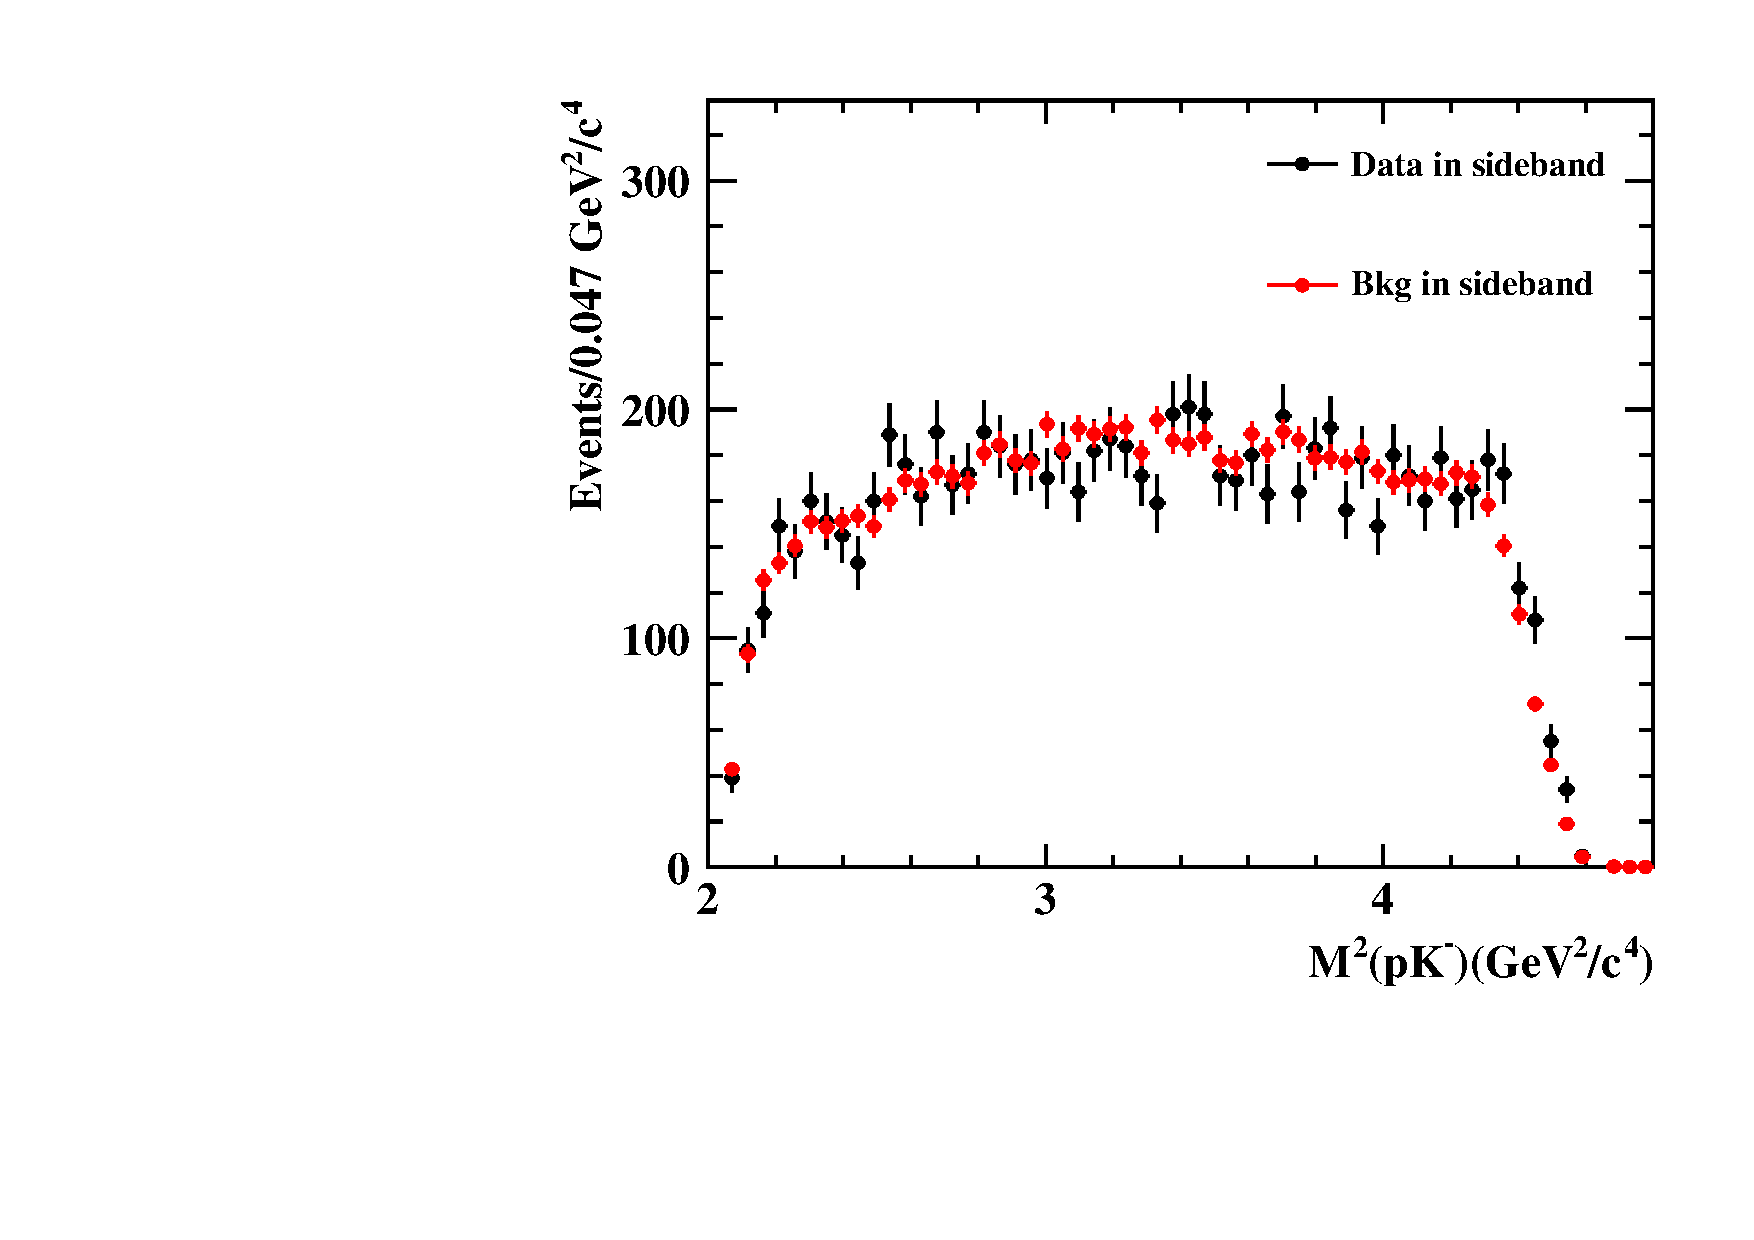
\includegraphics[width=0.325\textwidth]{figure/sideband/output_data_mc_0_sideband_m2_12_2c_1.pdf}
    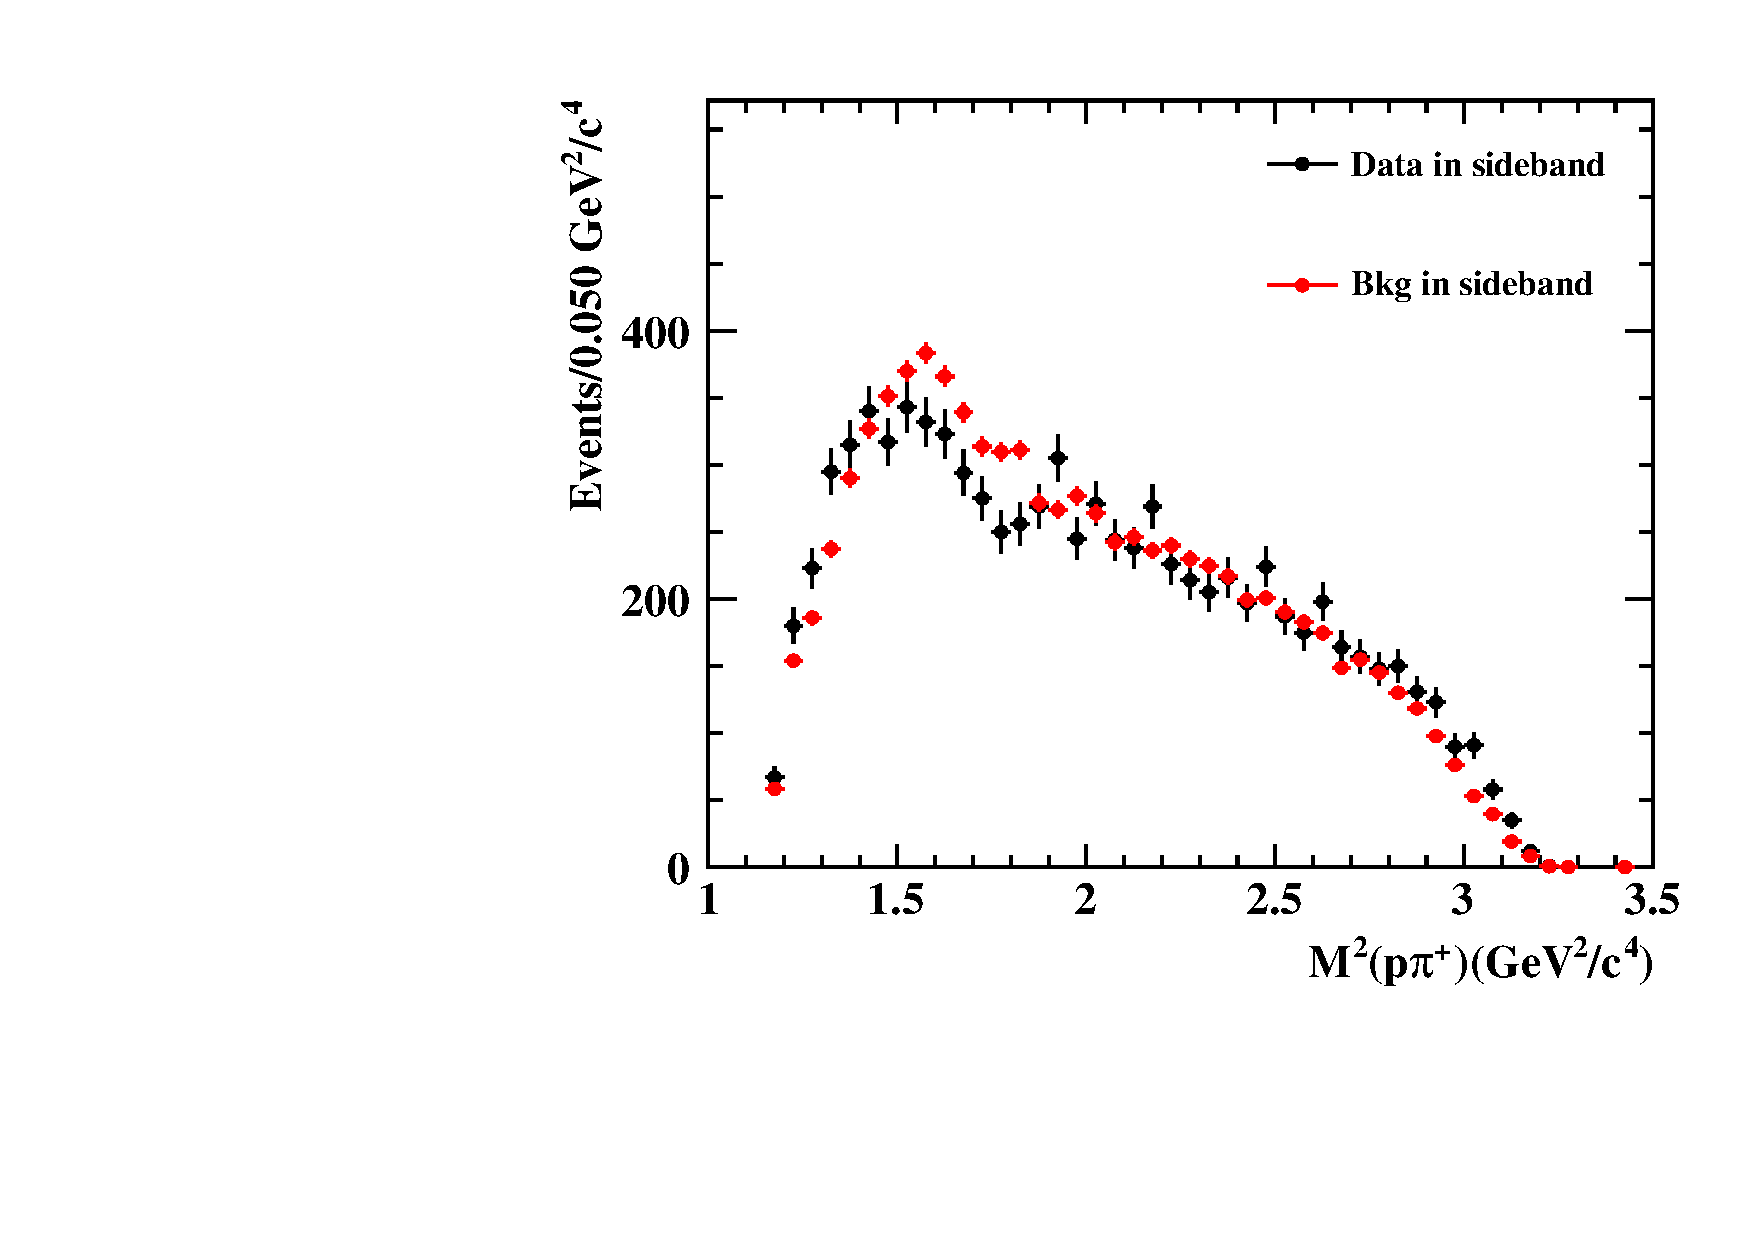
\includegraphics[width=0.325\textwidth]{figure/sideband/output_data_mc_0_sideband_m2_13_2c_1.pdf}
    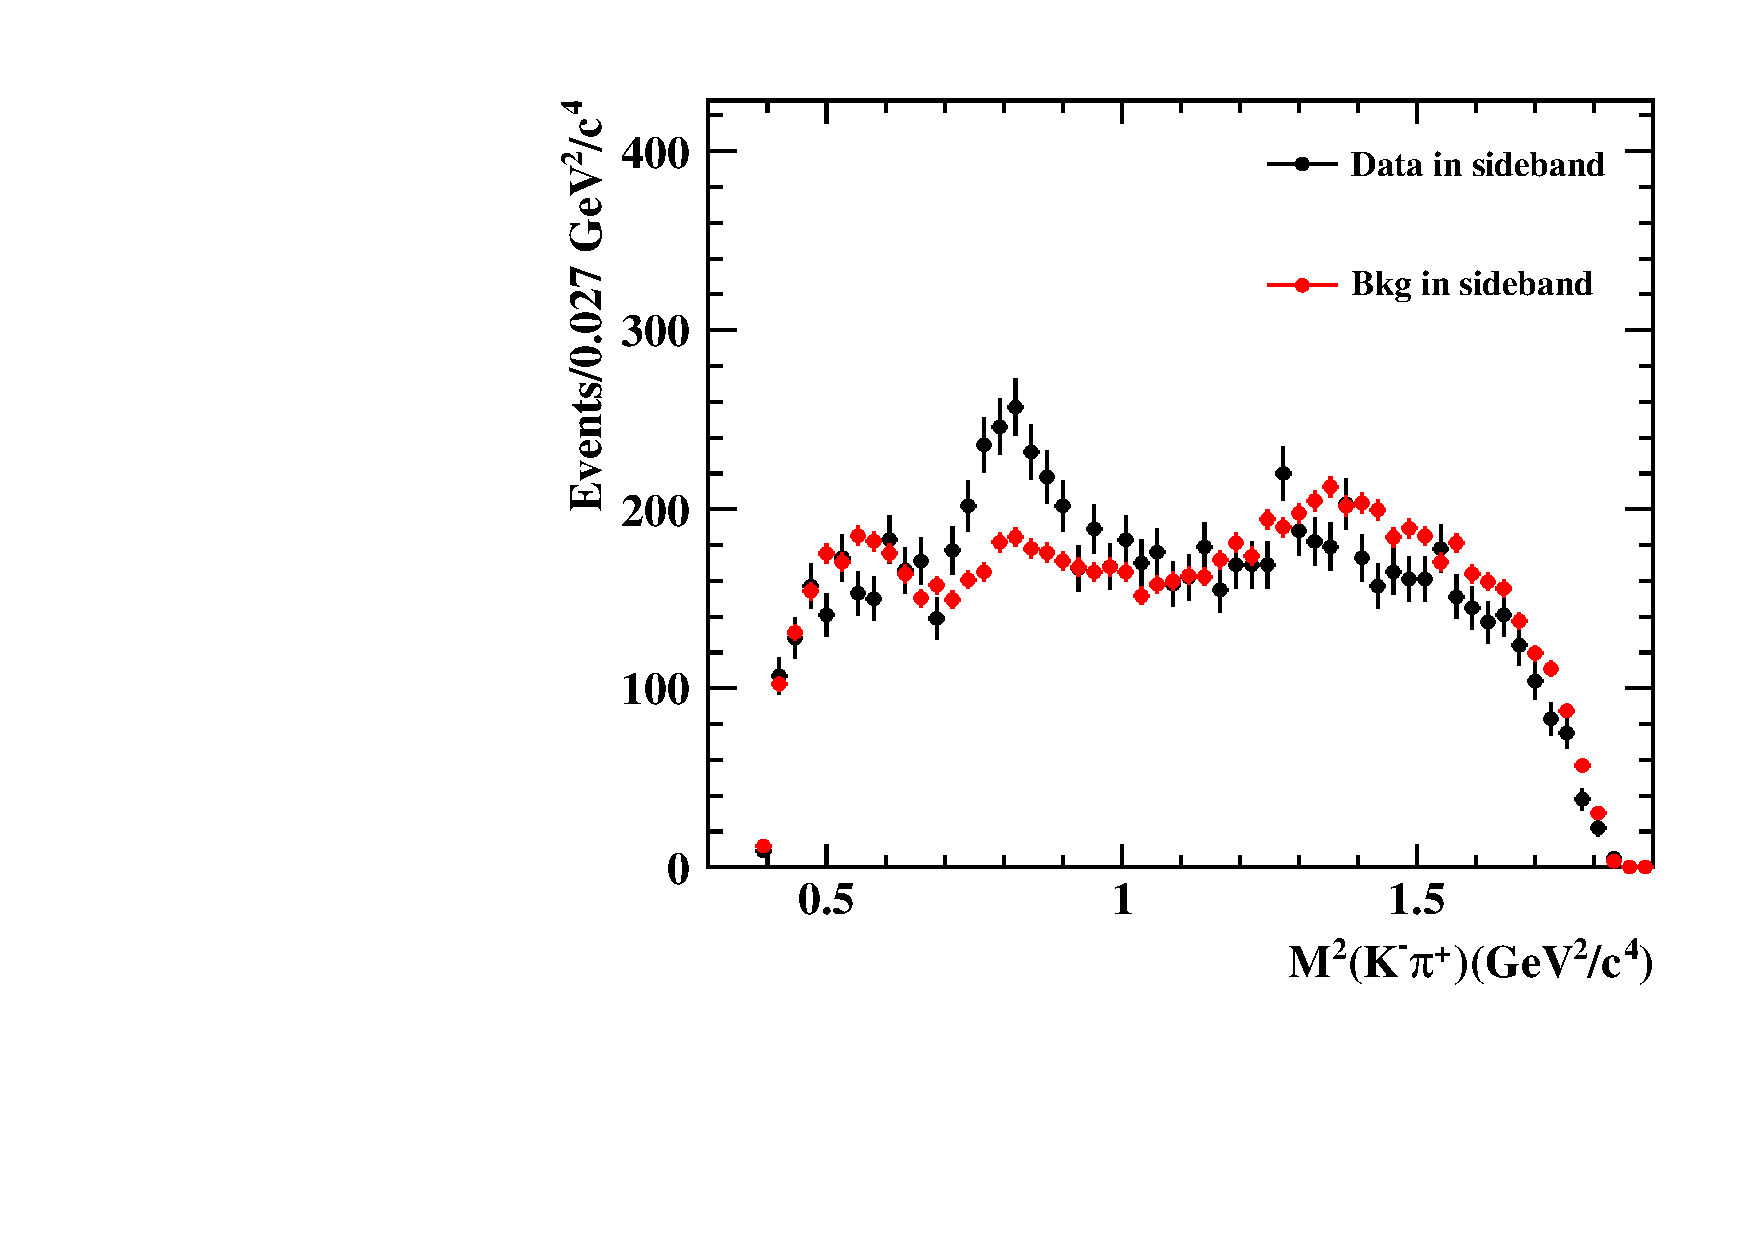
\includegraphics[width=0.325\textwidth]{figure/sideband/output_data_mc_0_sideband_m2_23_2c_1.pdf}
    \caption{Shape comparison of $M^2(pK^-)$ (left), $M^2(p\pi^+)$ (middle) and $M^2(K^-\pi^+)$ (right) between data and cocktail MC in the $\mbc$ sideband region.}
\label{fig:comp_datamc_sideband}
\end{figure}